\chapter{Event Reconstruction \& Selection}\label{chap:reconstruction}

Reconstruction is the process in a given event of building actual physics processes, such as an $\aprime$ decay, from the raw hits of the detector channels readout by the trigger. The HPS event reconstruction is based on the lcsim software toolkit \cite{Graf_2011} and uses both reconstructed energy clusters from the Ecal and tracks from the SVT, which are done independently until Ecal clusters and tracks are matched by extrapolating the track state at the last layer of the SVT to a cluster in the Ecal for particle identification. These objects, mainly $e^+e^-$ pairs or $e^-e^-$ pairs, are used to reconstruct vertices used for the physics analysis. The multiple stages of the HPS reconstruction - SVT hit reconstruction, tracking, vertexing, and Ecal clusters - are discussed in the following sections.

\section{HPS Coordinate Systems}\label{sec:coordinates}

\begin{table}[!hb] 
\centering
\begin{tabular}{lccc}
   \toprule    
    Coordinate System & $x$ & $y$ & $z$ \\
    \midrule
     JLab Coordinates & Beam left & Vertical & Beam direction \\
     Detector/HPS Coordinates & Beam left rot. -30.5 mrad & Vertical & Beam direction rot. -30.5 mrad \\
     Tracking/lcsim Coordinates & Beam direction & Beam left & Vertical \\
     \bottomrule
\end{tabular}
\caption{Basis for several different coordinate systems used in the HPS reconstruction and analysis.}
\label{table:coordinates}
\end{table}

\begin{figure}[t]
    \centering
    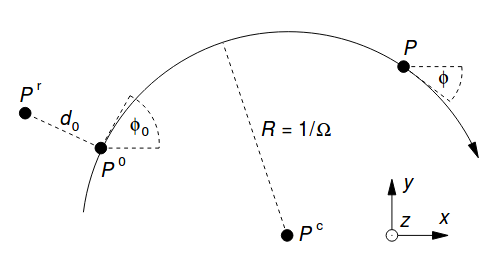
\includegraphics[width=.5\textwidth]{figs/recon/lcsim_1.png}
    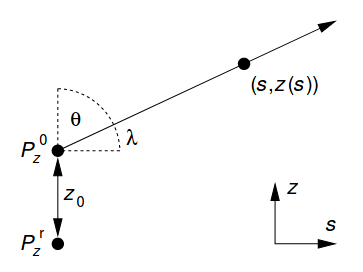
\includegraphics[width=.4\textwidth]{figs/recon/lcsim_2.png}
    \caption{A schematic of the linear collider tracking parameters \cite{Kraemer:81214}. %http://flc.desy.de/lcnotes/notes/localfsExplorer_read?currentPath=/afs/desy.de/group/flc/lcnotes/LC-DET-2006-004.pdf
    }
    \label{fig:track_params}
\end{figure}

There are three coordinate systems utilized in the HPS reconstruction process - the global coordinates (JLab coordinates), the HPS coordinate system (detector coordinates), and tracking coordinates (lcsim coordinates). Each coordinate system is used in a different part of the reconstruction process since each has simplifying features. First, the JLab coordinate system is defined globally by the Hall B beamline where the the $x$-axis points beam left in the bend plane, the $y$-axis points vertically upwards, and the $z$-axis points along the direction of the beam. The origin is set at the intersection of the nominal beam and nominal target position. Due to the asymmetry of HPS with respect to the chicane, where the beam is bent due to the first dipole magnet in the chicane by 30.5 mrad about the $y$-axis in the $-x$-direction, the HPS $z$-axis and $x$-axis are also rotated by 30.5 mrad. Since the beam travels in the $+z$-direction in HPS coordinates at the target, this is the natural reference frame for reconstructed particles and, unless otherwise stated, the physics analysis including positions and momenta will utilize this frame.

The entire HPS SVT lies within a roughly uniform vertical magnetic field, thus a charged particle trajectory will form a helix. Unfortunately, the coordinate systems for track reconstruction and analysis on HPS are different. HPS utilizes perigee parametrization of tracks that fixes a magnetic field along the $z$-axis (which is the $y$-axis in HPS coordinates). The tracking coordinates are oriented approximately such that the $x$-axis points along the direction of the beam, the $y$-axis points beam left, and the $z$-axis points vertically upwards. In addition, each track is defined by 5 track parameters - $\Omega$, $d0$, $z0$, $tan \lambda$, and $\phi$ - and are briefly described below and shown in Fig. \ref{fig:track_params} \cite{Kraemer:81214}.

\begin{enumerate}
  \item $\Omega$ is the signed curvature of the track (i.e. the inverse of the radius $C=-q/R$).
  \item $d0$ is the signed impact parameter in the $xy$ tracking plane. In the HPS detector frame, this translates to the impact parameter along the $x$ (horizontal) direction.
  \item $z0$ is the tracking $z$ position at the point of closest approach to the reference point. This is the key tracking parameter for the isolation cut. In the HPS detector frame, this approximately corresponds to the impact parameter in the $y$ (vertical) direction.
  \item tan$\lambda$ is the slope of the straight line in the $sz$ tracking plane. In the HPS detector frame, this translates to the slope of the track $dy/dz$ in the $yz$ plane.
  \item $\phi$ is the azimuthal angle of the momentum of the particle at point of closest approach to the reference point.
\end{enumerate}

Due to multiple scattering in the silicon sensors, each segment of the track between scattering planes is described by a separate helix, called a track state. Thus, each track segment will have its unique 5 track parameters as well as a unique 5 $\times$ 5 covariance matrix of these track parameters, and a track will have 11 or 13 track states depending on the number of hits on track. This process is described in Sec \ref{sec:tracking}. The last importnat tracking parameter is the path length of the helix, denoted as $s$, which is useful for parametrization of the helix.

\section{Ecal Reconstruction}\label{sec:ecal_recon}

Electromagnetic particles that are incident on the Ecal and shower within the Ecal deposit energy in several crystals which can then be clustered together to give both the total energy deposited and an estimate of the hit position on the front face of the Ecal. The Ecal reconstruction is the process of building particle clusters from the waveforms readout in single crystals of the Ecal for a given event. Ecal crystals that are readout store 100 samples in 4 ns intervals relative to the trigger time. The pulse shape is fit with a three-pole function 

\begin{equation}
    F_{3pole}(t) = \frac{t^2}{2 \tau^3}e^{-\frac{t}{\tau}}
    \label{eqn:ecal_recon}
\end{equation}

The time constant $\tau$ is calibrated offline for each channel and is typically $\sim 2.4$ ns. From this function, the pedestal, time of the pulse, and amplitude are fit in offline reconstruction and pileup is ignored. From the amplitude, the pulse is converted to energy by two types of channel calibrations - cosmic rays and elastic scatters in the target \cite{ecalpulse}. Cosmic rays, which pass downward through the Ecal and deposit a calculable amount of energy in the crystals, are used for a preliminary Ecal calibration before data taking. After data taking, cluster energy is calibrated with electrons elastically scattered by the target, which are very near the beam energy, and the gain constants for every crystal are adjusted until the energies match what is observed in MC. Cosmic ray MIPs and elastically scattered electrons sample the full range of interest in energy.

%Cosmic rays are calibrated before data taking with the beam off through the detection of minimum ionizing particles (MIPs), which have a known rate of energy loss, passing downwards through the Ecal.

%Cosmic rays, which pass downward through the ECal and deposit a calculable amount of energy in the crystals, are used for a preliminary Ecal calibration.

In order to form clusters in the Ecal, individual hits are grouped together using a clustering algorithm adapted from the CLAS Inner Calorimeter \cite{ASRYAN2020163425}. A crystal which has the most energy in a local group of hits becomes the seed for a cluster, and the algorithm looks for hits in neighboring crystals which are within 8 ns of the seed to build the cluster. Since higher energy hits have better timing resolution, the seed hit time is defined as the time of the cluster. %The seed hit time is used as the time of the cluster with larger energy since higher energy hits have better timing resolution. %Hits with a local energy maxima are seeded for clusters, and then the algorithm searches for neighboring crystals with seeds or a hit on a cluster within 8 ns of the seed. The seed hit time is used as the time of the cluster with larger energy since higher energy hits have better timing resolution. 

The energy of the cluster is initially the sum of the individual hit energies. However, this energy does not account for parts of the electromagnetic showers that are lost on the Ecal edges or absorbed in the vacuum flanges. In addition, particles generally enter an Ecal crystal at an angle off axis from crystal axis and electromagnetic showers deposit energies at all Ecal depths resulting in the fact that maximum energy deposition may not occur in the same crystal as the crystal whose front face the particle has traversed. As a result, energy corrections are based on detailed MC studies and the energy is corrected as a function of particle type (photon, electron, or positron), energy, and angle, where the particle type must be determined by track-cluster matching later in the reconstruction described in Sec. \ref{sec:trackcluster}. In addition, the position of the cluster is initially determined by a logarithmically-weighted centroid. For the same reason as energy, the position must also be corrected and is done so in the same MC studies as energy \cite{ecalsim} \cite{ecalenergy}.

\clearpage

\section{SVT Reconstruction} \label{sec:svtrecon}

The SVT reconstruction is the process of building particle tracks from the collection of waveforms readout from all the single strips in the SVT which have been hit. These tracks are used to form electron and positron objects (tracks matched with Ecal clusters), which are then used to form vertices used in the final analysis.

\subsection{SVT Hit Reconstruction}
For each trigger, SVT channels where at least three of the six samples are above the readout threshold, that was determined by offline calibration before data taking in calibration runs (for reasons described in Sec. \ref{sec:svt_daq}), are readout. For each strip in the SVT that is readout, the APV25 reads out six samples at 24 ns intervals. The APV25 response is modeled as a four pole filter with three coincident poles (i.e. three of the poles with the same time constant). This gives the following transfer function with two time constants $\tau_1$ and $\tau_2$.

\begin{equation}
    \tilde{F}(\omega)=\frac{1}{(1+i \omega \tau_1)(1+i \omega \tau_2)^3}
    \label{equ:transfer}
\end{equation}

The inverse Fourier Transform of this transform function is the pulse shape given by

\begin{equation}
    F(t,\tau_1,\tau_2)=A \frac{\tau_1^2}{(\tau_1-\tau_2)^3} \left(  e^{-\frac{t-t_0}{\tau_1}}-\sum_{k=0}^2 \left( \frac{\tau_1-\tau_2}{\tau_1 \tau_2}(t-t_0) \right)^k \frac{e^{-\frac{t-t_0}{\tau_2}}}{k!} \right)
    \label{equ:sample_fits}
\end{equation}

The time constants are predetermined offline by fitting pulses in calibration runs and have typical values of $\tau_1 \approx 72$ ns and $\tau_2 \approx 12$ ns. $t_0$ is defined as the time the fit crosses 0 and is set as the time of the raw hit. $A$ is related to the amplitude of the pulse in ADC counts. Both of these quantities are determined by the fit in offline reconstruction and an example waveform and fit is shown in Fig. \ref{fig:6samples}.

The pulse is fit to a pileup algorithm where a fit to a single pulse is compared to a fit with a double pulse. If the single pulse fit has a $\chi^2$ probability less than 0.5, a refit with two pulses is attempted. If this produces an improved $\chi^2$ probability, the double pulse fit is accepted, else the single pulse fit is accepted. The time of the pulse is corrected after the fit for several effects including a run-dependent phase shift, trigger time, and time of flight. %The $t_0$ is corrected in reconstruction for several affects. First, $t_0$ is corrected by a run-dependent phase shift or offset time. Then $t_0$ corrected for the trigger time. Then trigger hitter and the time scale is subtracted (55). Then, subtract $t_0$. The $t_0$ is shifted sensor-by-sensor. Then time of flights corrects are applied based on sensor position. /textcolor{red}{I am very confused by all these time shifts - Matt S.}

\begin{figure}[t]
    \centering
    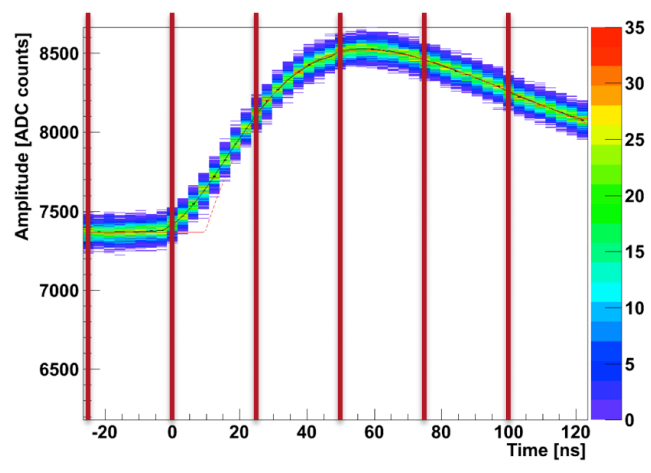
\includegraphics[width=.85\textwidth]{figs/recon/6samp.png}
    \caption{A plot of the digitized waveform that is output from the APV25 and is fit using Eq. \ref{equ:sample_fits}. The 6 samples used for the fit are in 24 ns intervals (between the red lines).
    }
    \label{fig:6samples}
\end{figure}

\clearpage

\subsection{SVT Cluster and 3D Hit Reconstruction}
After single strip hit reconstruction, the hits are clustered together with neighboring hits using the nearest neighbor RMS Clusterer algorithm. The algorithm uses the amplitudes in ADC counts (where it is not necessary to convert amplitude to energy deposition) and seeds hits whose amplitude are at least 4$\sigma$ above the noise of the channel, where $\sigma$ is the RMS of the noise of the channel. From there, it appends neighboring strips whose pulse times are within 8 ns of the seed strip and whose amplitudes are at least 3 RMS above the noise of the channel. In addition, each of the strips, whether seed or neighbor channel, must have a $\chi^2$ probability for the fit in Eq. \ref{equ:sample_fits} greater than $3.20 \times 10^{-6}$.  %($Q(4,20)$ where Q is the regularized gamma function). 
The position of the cluster is the amplitude-weighted centroid of the hits ($\sum x_i A_i/\sum A_i$). Typically, SVT clusters are composed of one or two strips hits in approximately equal proportion. Since time resolution is significantly degraded for hits with low energy deposition, the time of the SVT cluster is weighted by the square of the amplitude ($\sum t_i A_i^2/\sum A_i^2$).

The 1D strip clusters in each axial sensor in a given layer are then paired together with the corresponding stereo sensor in the same layer to form 3D hits. Only clusters within 12 ns of the trigger time and with at least an amplitude of 400 ADC counts are considered. As a reference, a minimum ionizing particle (MIP) will typically have an amplitude of $\sim 1200$ ADC counts. These clusters must cross physically in space from the perspective of the primary (with some tolerance) and be within a 16 ns coincidence of each other. A 3D hit is reconstructed at the intersection of the two strip clusters. Since this intersection depends on the track angle, the 3D hit position is recalculated every time the hit is used in a track fit to correct for parallax effects.

\clearpage

\subsection{Track Reconstruction} \label{sec:tracking}

The SeedTracker algorithm, which was developed for design studies with the SiD detector \cite{seedtracker}, is performed as a simple method of track finding for HPS. Seed tracks, that is tracks that result from SeedTracker, are found using several different track finding strategies. The tracking strategies are as follows.

\begin{enumerate}
  \item A track candidate is found using a particular three (of the six possible) 3D hits to form a helical track.
  \item This helix is extrapolated to a confirm layer and, if this confirm layer has a 3D hit consistent with the helix, this hit is appended to the helical trajectory. Else, the track candidate is discarded.
  \item Lastly this 4-hit track is extrapolated to the remaining two layers called the extend layers. The 3D hits in those layers that are consistent with the helix are appended. We require at least one of the extend layers to have a 3D hit consistent with the helix, thus requiring a minimum of five 3D hits on a track. If this extend requirement is not met, the track candidate is discarded.
\end{enumerate}

%Initially, a track candidate is found using three 3D hits which forms a helical track. This helix is extrapolated to a confirm layer and, if this confirm layer has a 3D hit consistent with the helix, this hit is appended to the helical trajectory. Else, the track candidate is discarded. Lastly this track is extrapolated to the remaining two layers called the extend layers, and appends the 3D hits in those layers that are consistent with the helix. We require at least one of the extend layers to have a 3D hit consistent with the helix, thus requiring a minimum of five hit tracks. If this extend requirement is not met, the track candidate is discarded. 

Four tracking strategies are used because any single strategy using this method will not find tracks that happen to miss a seed or confirm layer. The four tracking strategies used in the reconstruction are s-345 c-2 e-16, s-456 c-3 e-21, s-123 c-4 e-56, and s-123 c-5 e-46 where s, c, and e are abbreviations for seed, confirm, and extend, respectively. As an example, s-345 c-2 e-16 seeds track candidates using 3D hits on layers 3, 4, and 5. Then, this helical fit is extrapolated to layer 2, followed by layers 1 and 6. The seed tracks from 345 that successfully append a hit in layer 2 and either layer 1 or 6 are stored as a track candidate to be used for the remaining reconstruction.

In addition, there are several other requirements the track must pass. The RMS time of all the hits on the track must fall within 8 ns. The track must have a $\chi^2$ less than 100 (including an individual hit $\chi^2$ less than 10), a distance of closest approach $d0$ less than 15 mm, an impact parameter $z0$ of less than 15 mm, and a minimum transverse momentum of 100 MeV. 

The SeedTracker algorithm returns a helical track fit to 3D hits, but fails to take multiple scattering into account which results in an artificially worsened momentum resolution. In order to account for multiple scattering effects, the helical track fit is refit using the General Broken Lines (GBL) algorithm \cite{BLOBEL200614} \cite{Kleinwort_2012}. For HPS, the GBL algorithm treats each sensor plane in the SVT as a source of scattering and fits a track segment (defined by 5 parameters described in Sec. \ref{sec:coordinates} that define the track state) between each sensor plane and extrapolates a track segment on the first and last SVT sensor plane. For the reconstruction of the 2016 Engineering Run dataset, the GBL track is required to have a $\chi^2$ per degree of freedom less than 12. The GBL fit minimizes the hit residuals and scattering angles (called kinks) for each of these track segments and provides performance equivalent to a Kalman filter. However, the GBL implementation for HPS requires 3D hits from SeedTracker before inputting the track into the GBL algorithm. This 3D hit requirement results in some efficiency loss due to acceptance for particles that only traverse either the axial or stereo sensor in a given layer. In addition, there are further efficiency losses due to the inherent efficiency effects of individual sensors where an inefficiency in either the axial or stereo sensor will not form a 3D hit. For future track reconstruction for HPS, a Kalman filter that utilizes strip hits for pattern recognition instead of 3D hits will be used to regain this loss of efficiency.

A plot of the hit efficiency for each SVT layer separated by hemisphere and curvature is shown in Fig. \ref{fig:hitefflay}. Layer 1 has decreased hit efficiency due a larger occupancy than the rest of the detector, while layer 6 has decreased hit efficiency due to a large number of dead channels in that layer. Positrons also have a decreased layer 1 efficiency due to wide-angle bremsstrahlung conversions in layer 1 in which a positron track extrapolates to layer 1 but may not leave a hit. The methods of measuring hit efficiency as well as separating the measurement by channel will be described in more detail in Sec. \ref{sec:hiteff}.

\begin{figure}[t]
    \centering
    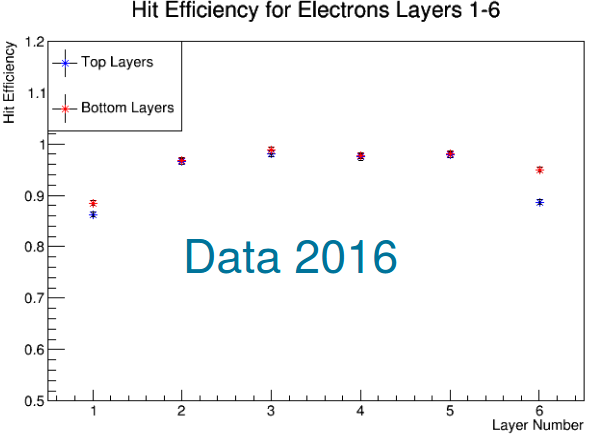
\includegraphics[width=.45\textwidth]{figs/recon/hitefflayele.png}
    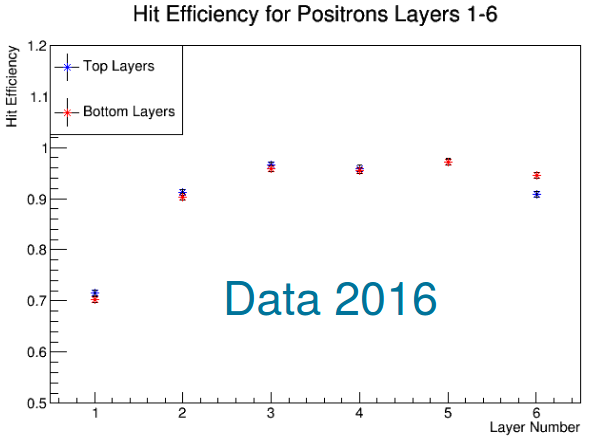
\includegraphics[width=.45\textwidth]{figs/recon/hitefflaypos.png}
    \caption{The hit efficiency for each top/bottom layer of the SVT for Left: electrons and Right: positrons. The decrease in efficiency in layer 1 and layer 6 can be attributed to increased occupancy and a large number of dead channels, respectively. The difference between electrons and positrons in layer 1 hit efficiency is a result of WABs, where a conversion occurs in layer 1 and fails to produce a hit in both axial and stereo sensors, which is measured as a hit inefficiency.
    }
    \label{fig:hitefflay}
\end{figure}

\clearpage

\section{Track Cluster Matching} \label{sec:trackcluster}
Tracks are matched to Ecal clusters by extrapolating the track state of the final SVT hit to the face of the Ecal though a non-uniform magnetic field map, which accounts for the dipole magnet's fringe field, and comparing this extrapolated position to the Ecal cluster position. Matching a track to an Ecal cluster confirms the reality of the track since all particles of interest that produce a track should also form an Ecal cluster.\footnote{In reality, particles of interest (typically electrons) can produce tracks but extrapolate to the so-called ``Ecal hole'' which was cut out to reduce occupancy from elastically-scattered beam particles. These tracks can be recovered by implementing a positron-only trigger and relaxing the requirement of an electron track matched to an Ecal cluster. This is done in the upgraded detector for future running described in Sec. \ref{sec:L0}.} In addition, since the Ecal offers a better time estimate than tracking, the time coincidence of two Ecal clusters can be used to reduce the effects of accidentals.

The track is matched with the cluster with the minimum $n_{\sigma}$, where $\sigma$ is the error on the extrapolated track position from layer 6 of the SVT to the front face of the Ecal , provided that the match is less than 30$\sigma$. Subsequent analysis imposes a stricter requirement. An electron object is defined as a negatively curved GBL track that is matched to an Ecal cluster in the same detector volume. Similarly, a positron object is defined as a positively curved GBL track that is matched to an Ecal cluster in the same detector volume. The electron and positron objects are used as inputs to the vertex fitter. The remaining Ecal clusters that do not have an associated matching track are defined as photon objects. At this beam energy, some muons and pions are present, but the vast majority of charged particles are electrons and positrons. Thus, nearly all the energy deposition in the Ecal is a result of electrons, positrons, and photons.

To potentially further reduce accidentals, one might expect the ratio of the energy of the Ecal cluster to the momentum of the matched track ($E/p$) to have a mean at one with a small $\sigma$ corresponding to the energy and momentum resolutions. However, the particles near the edge of the Ecal, where much of the action occurs, typically only deposit a fraction of their energy into the Ecal crystals. Thus, $E/p$ is non-Gaussian with a mean below 1 and as a result, no restriction on $E/p$ is imposed.

\clearpage

\section{Vertexing}

\begin{table}[t] 
    \centering
    \begin{tabular}{lr}
        \toprule
        \textbf{Cut Description} & \textbf{Requirement} \\
        \midrule
        Cluster Time Difference & $|t_{e^+ Cluster}-t_{e^- Cluster}|<2.5$ ns\\
        $e^{+}$ Track-Cluster Time Difference & $|t_{e^+ Track}-t_{e^+ Cluster} - 55| < 10$ ns\\
        $e^{-}$ Track-Cluster Time Difference & $|t_{e^- Track}-t_{e^- Cluster} - 55| < 10$ ns\\
        Ecal clusters in opposite volumes 
        	& $y_{\posi \mathrm{ Cluster}} \times y_{\ele \mathrm{ Cluster}} < 0$ \\
        Loose track-cluster match & $\chi^2 < 15$  \\
        Beam electron cut & $p(e^{-}) < 2.15$ GeV \\
        Track Quality & $\chi^2/dof < 12$ \\
        Maximum Vertex Momentum & $V_{0p} < 2.8$ GeV \\ 
        \bottomrule
    \end{tabular}
    \caption{Requirements applied to $V_{0}$ particles during the 
    		 reconstruction stage for data (i.e. preprocessing selection).}
    \label{tab:mouse_data}
\end{table}

\begin{table}[t] 
    \centering
    \begin{tabular}{lr}
        \toprule
        \textbf{Cut Description} & \textbf{Requirement} \\
        \midrule
        Cluster Time Difference & $|t_{e^+ Cluster}-t_{e^- Cluster}|<5$ ns\\
        Track-Cluster Time Difference & $|t_{e^+ Track}-t_{e^+ Cluster} - 43| < 10$ ns\\
        Track-Cluster Time Difference & $|t_{e^- Track}-t_{e^- Cluster} - 43| < 10$ ns\\
        Ecal clusters in opposite volumes 
        	& $y_{\posi \mathrm{ Cluster}} \times y_{\ele \mathrm{ Cluster}} < 0$ \\
        Loose track-cluster match & $\chi^2 < 15$  \\
        Beam electron cut & $p(e^{-}) < 2.15$ GeV \\
        Track Quality & $\chi^2/dof < 6$ \\
        Maximum Vertex Momentum & $V_{0p} < 2.8$ GeV \\ 
        \bottomrule
    \end{tabular}
    \caption{Requirements applied to $V_{0}$ particles during the 
    		 reconstruction stage for MC (i.e. preprocessing selection).}
    \label{tab:mouse_mc}
\end{table}

Every pair of $e^+$ and $e^-$ objects in an event is fitted to a Billior vertex fitter \cite{BILLOIR1992139}. The Billior vertex fit is a fast vertex fit that finds the best-fit vertex position and track parameters based on the individual track parameters and covariance matrices of the $e^+e^-$ pair. This provides a vertex with a reconstructed 3D position based on the distance of closest approach between the two tracks as well as a reconstructed mass and momentum that are determined based on the fitted track parameters at the fitted vertex position. 

Given a collection of vertices made up of electron and positron tracks, additional constraints can be imposed to reduce backgrounds. Any real heavy photon decay vertex will have tracks in opposite hemispheres of the detector, point back to the beamspot, and have a vertex momentum (the sum of the momenta of the two tracks) consistent with heavy photon kinematics. If the $e^+$ and $e^-$ objects are in the same hemisphere of the detector (most likely converted bremstrahlung), they are placed in the Unconstrained Vc Collection and not considered for this analysis. If the $e^+$ and $e^-$ objects are in opposite hemispheres of the detector and they pass the preprocessing selection (cuts in the reconstruction) described in Tables \ref{tab:mouse_data} and \ref{tab:mouse_mc}, then they are placed in the Unconstrained V0 Particle Collection and considered for the analysis. These standard loose restrictions come from previous analysis and will be stricter at the analysis stage. The descriptions and motivations for these cuts are described in detail in Sec. \ref{sec:preselection}.

In addition, a target constraint ($x$, $y$, and $z$ positions) and a beamspot constraint ($x$ and $y$ components of the V0 momentum) are put on the V0 particle. For a given V0 particle, the unconstrained, target constrained, or the beamspot constrained vertex fit can be used depending on the type of analysis being performed. Specifically, the target constraint requires the vertex to be consistent with the $z$ position of the target and the $x$ and $y$ positions and sizes of the beamspot while the beamspot constraint requires the vertex momentum to point back to the beamspot at the target $z$ position. Unconstrained vertices are used for the displaced vertex analysis while target constrained vertices are used for the resonance search. 

%and placed in separate collections with a one-to-one-to-one mapping between the three collections.

In addition, all electron object pairs are also fit with a Billior Vertex and placed in the unconstrained M\o ller Candidate Vertex Collection. M\o ller candidates are also fit with target and beamspot constraints in separate collections and mapped in the same way. The M\o ller candidates are used for the studying the data/MC comparison of the mass resolution as described in Sec. \ref{sec:massresolution}.

The beamspot and target constrained Billior vertices both use the beam position and size along with the target position in $z$ as an input. For data, a run-by-run beam parameters were selected based on the fits of distributions. Plots for these beam parameters are shown in Fig. \ref{fig:rundepposz} and Fig. \ref{fig:rundepposxy} where the data is shown as points and the MC is shown as a solid line. For simplicity, the parameters for MC are chosen to be constant and are $b_x=$ -0.224 mm, $\sigma_x=$0.125 mm, $b_y=$-0.08 mm, and $\sigma_y=$0.030 mm. These parameters were used for both the actual simulated beam position and profile as well as inputs to the Billior Vertexer. These parameters are also used as inputs to the event selection described in Sec. \ref{chap:aprimes}.

\begin{figure}[t!]
    \centering
    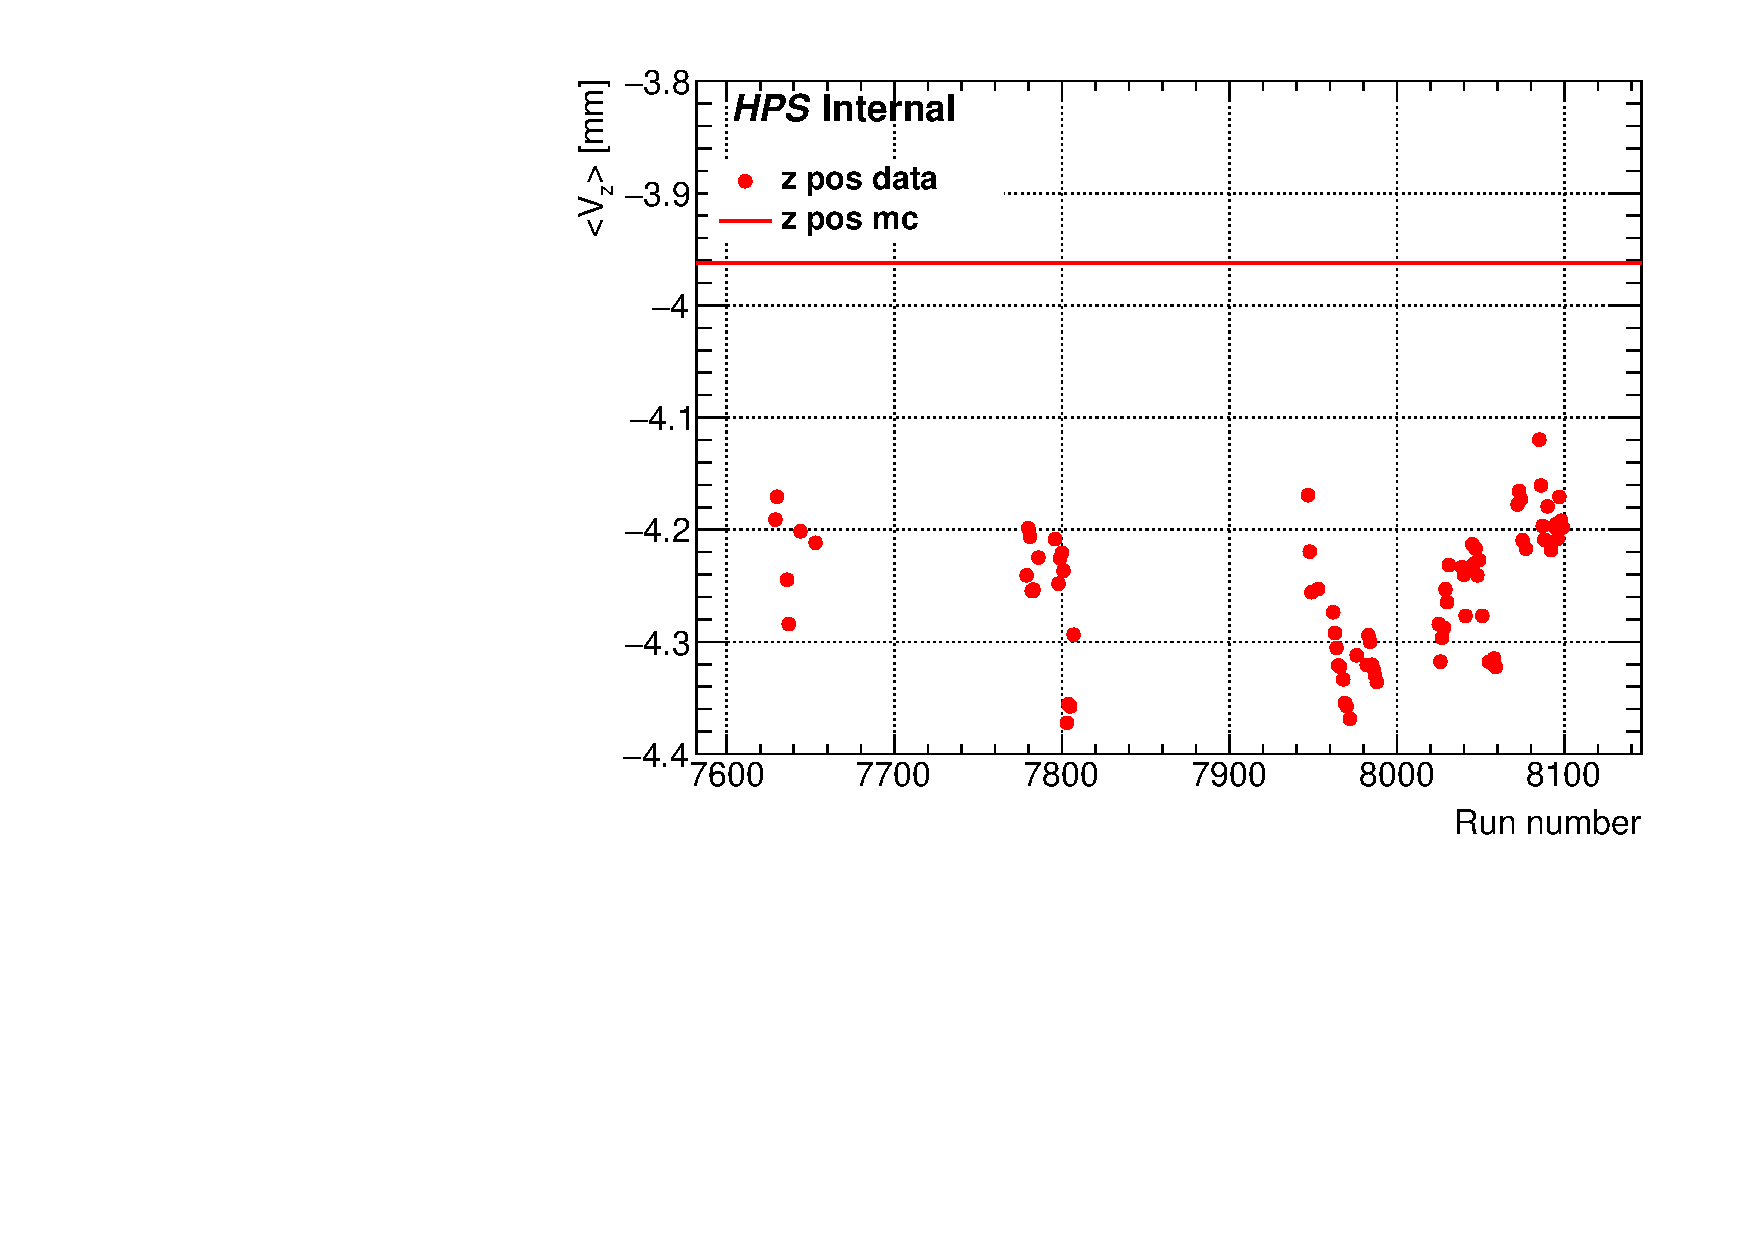
\includegraphics[width=0.85\textwidth]{figs/recon/z_final.pdf}
    \caption{The run-dependent average position in $z$ for unconstrained vertices fit represented by solid points and a solid line for data and MC simulation, respectively.}
    \label{fig:rundepposz}
\end{figure}

\begin{figure*}[t!]
    \centering
    %\begin{subfigure}[t]{0.45\textwidth}
    %    \centering
        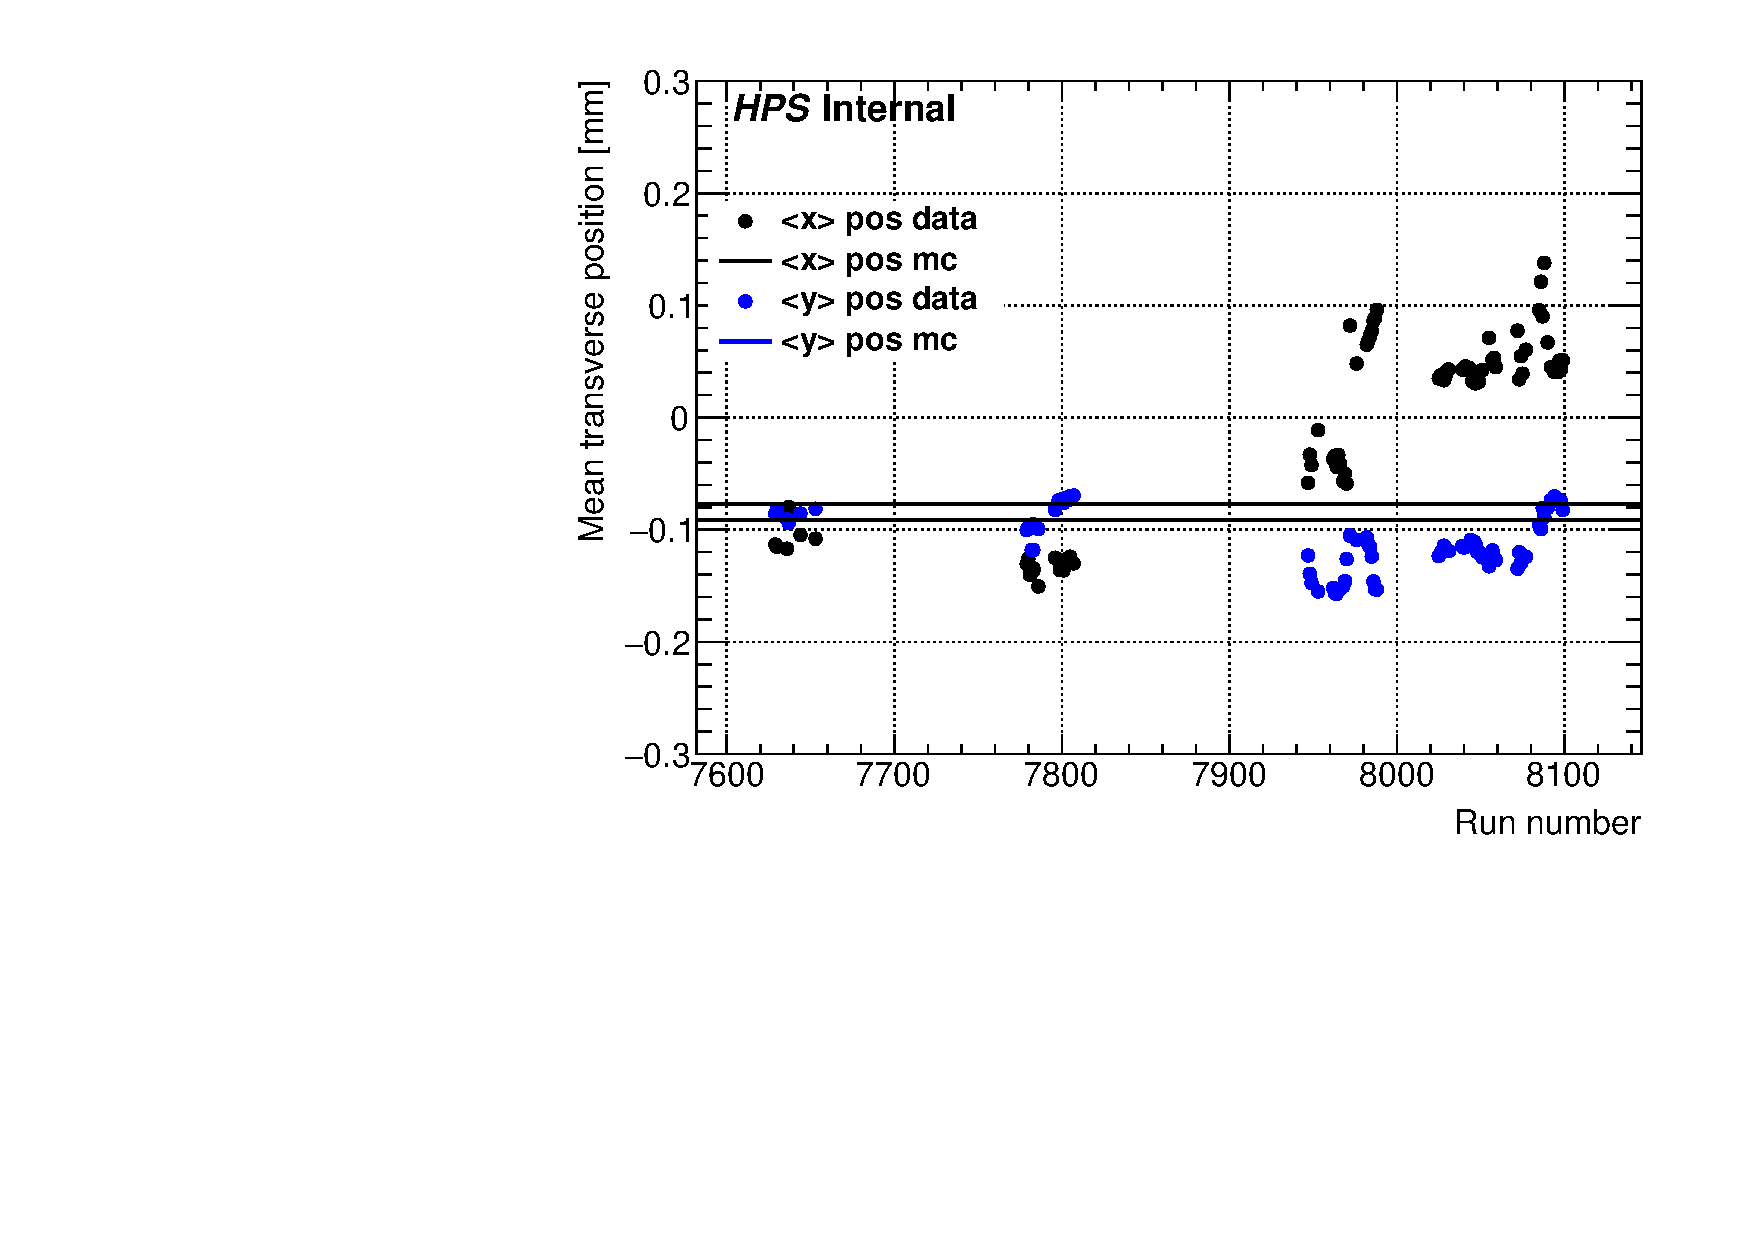
\includegraphics[width=.85\textwidth]{figs/recon/xy_final.pdf}
    %\caption{}
    %\end{subfigure}%
    %~ 
    %\begin{subfigure}[t]{0.45\textwidth}
    %    \centering
        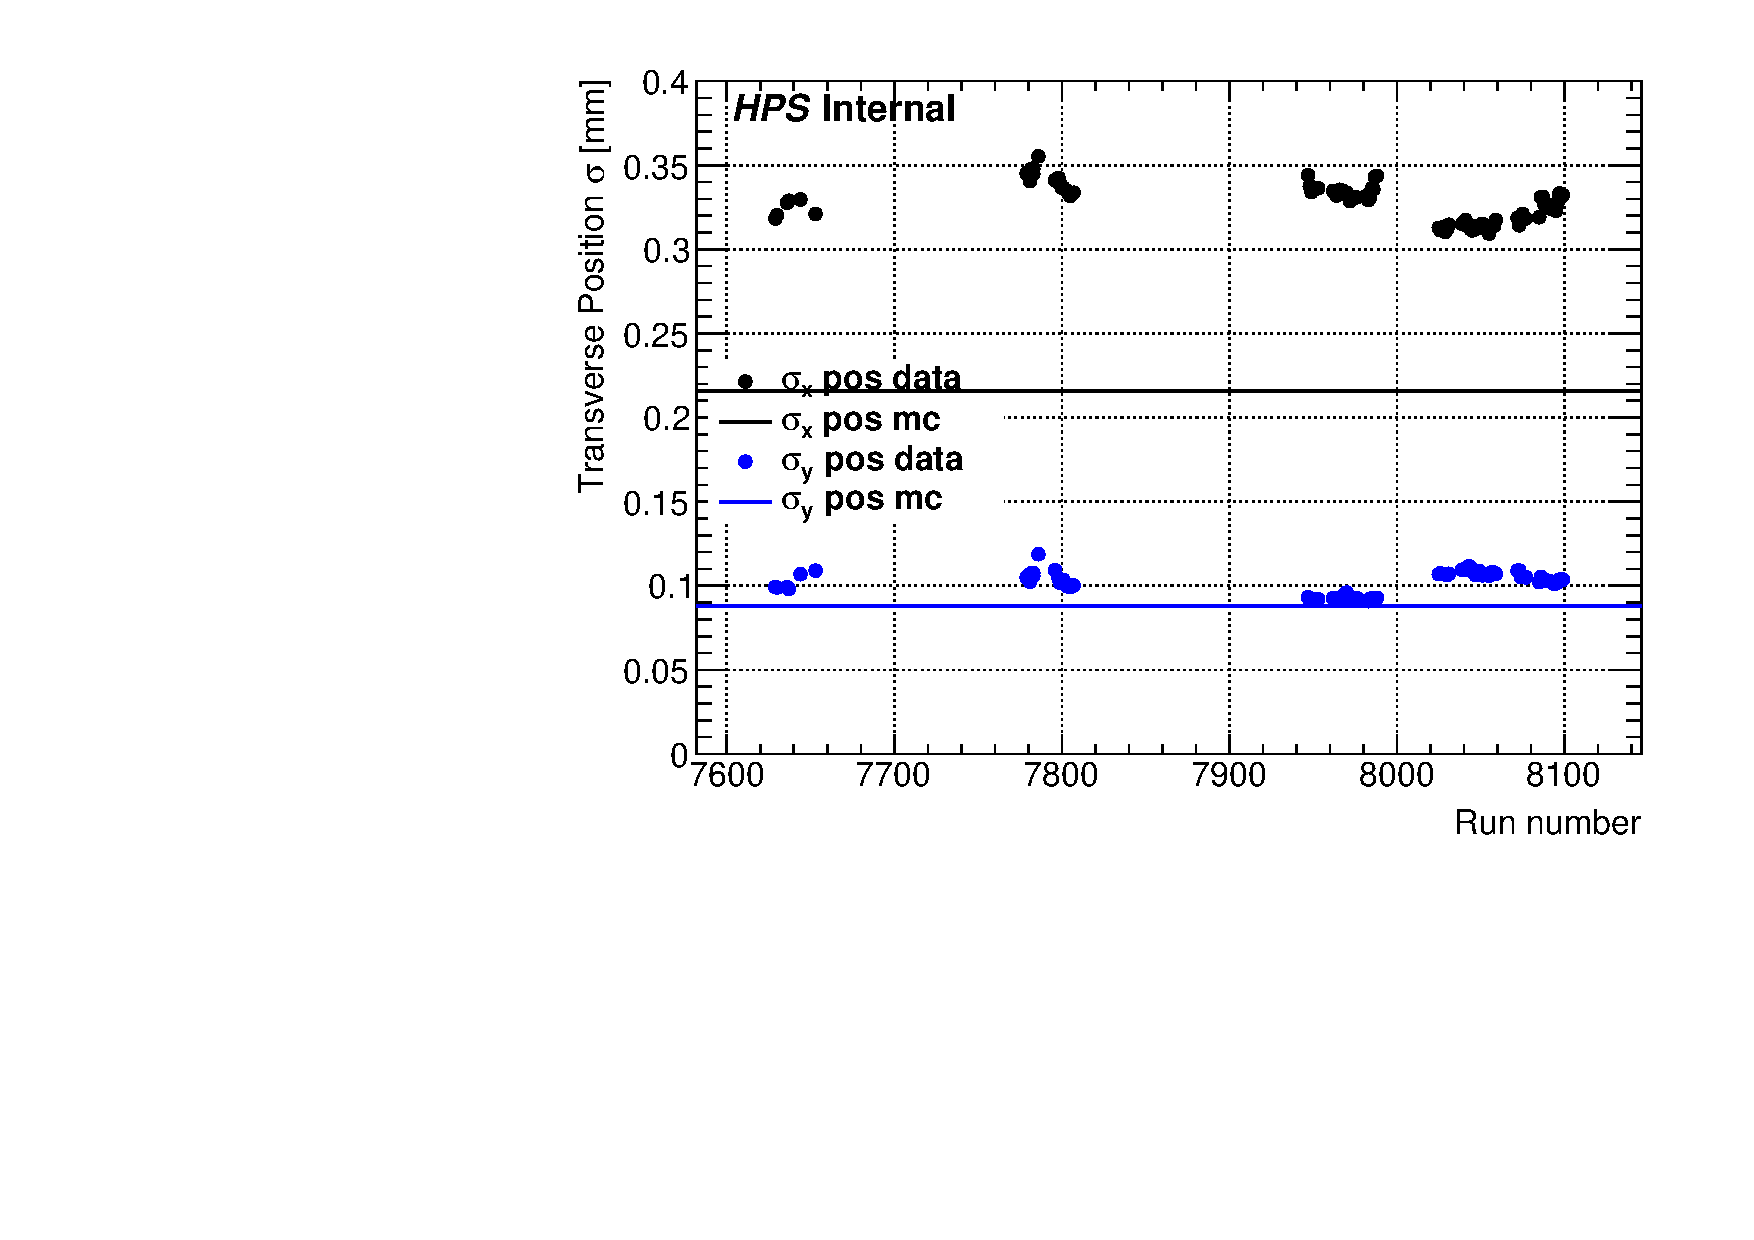
\includegraphics[width=.85\textwidth]{figs/recon/sigma_xy_final.pdf}
        %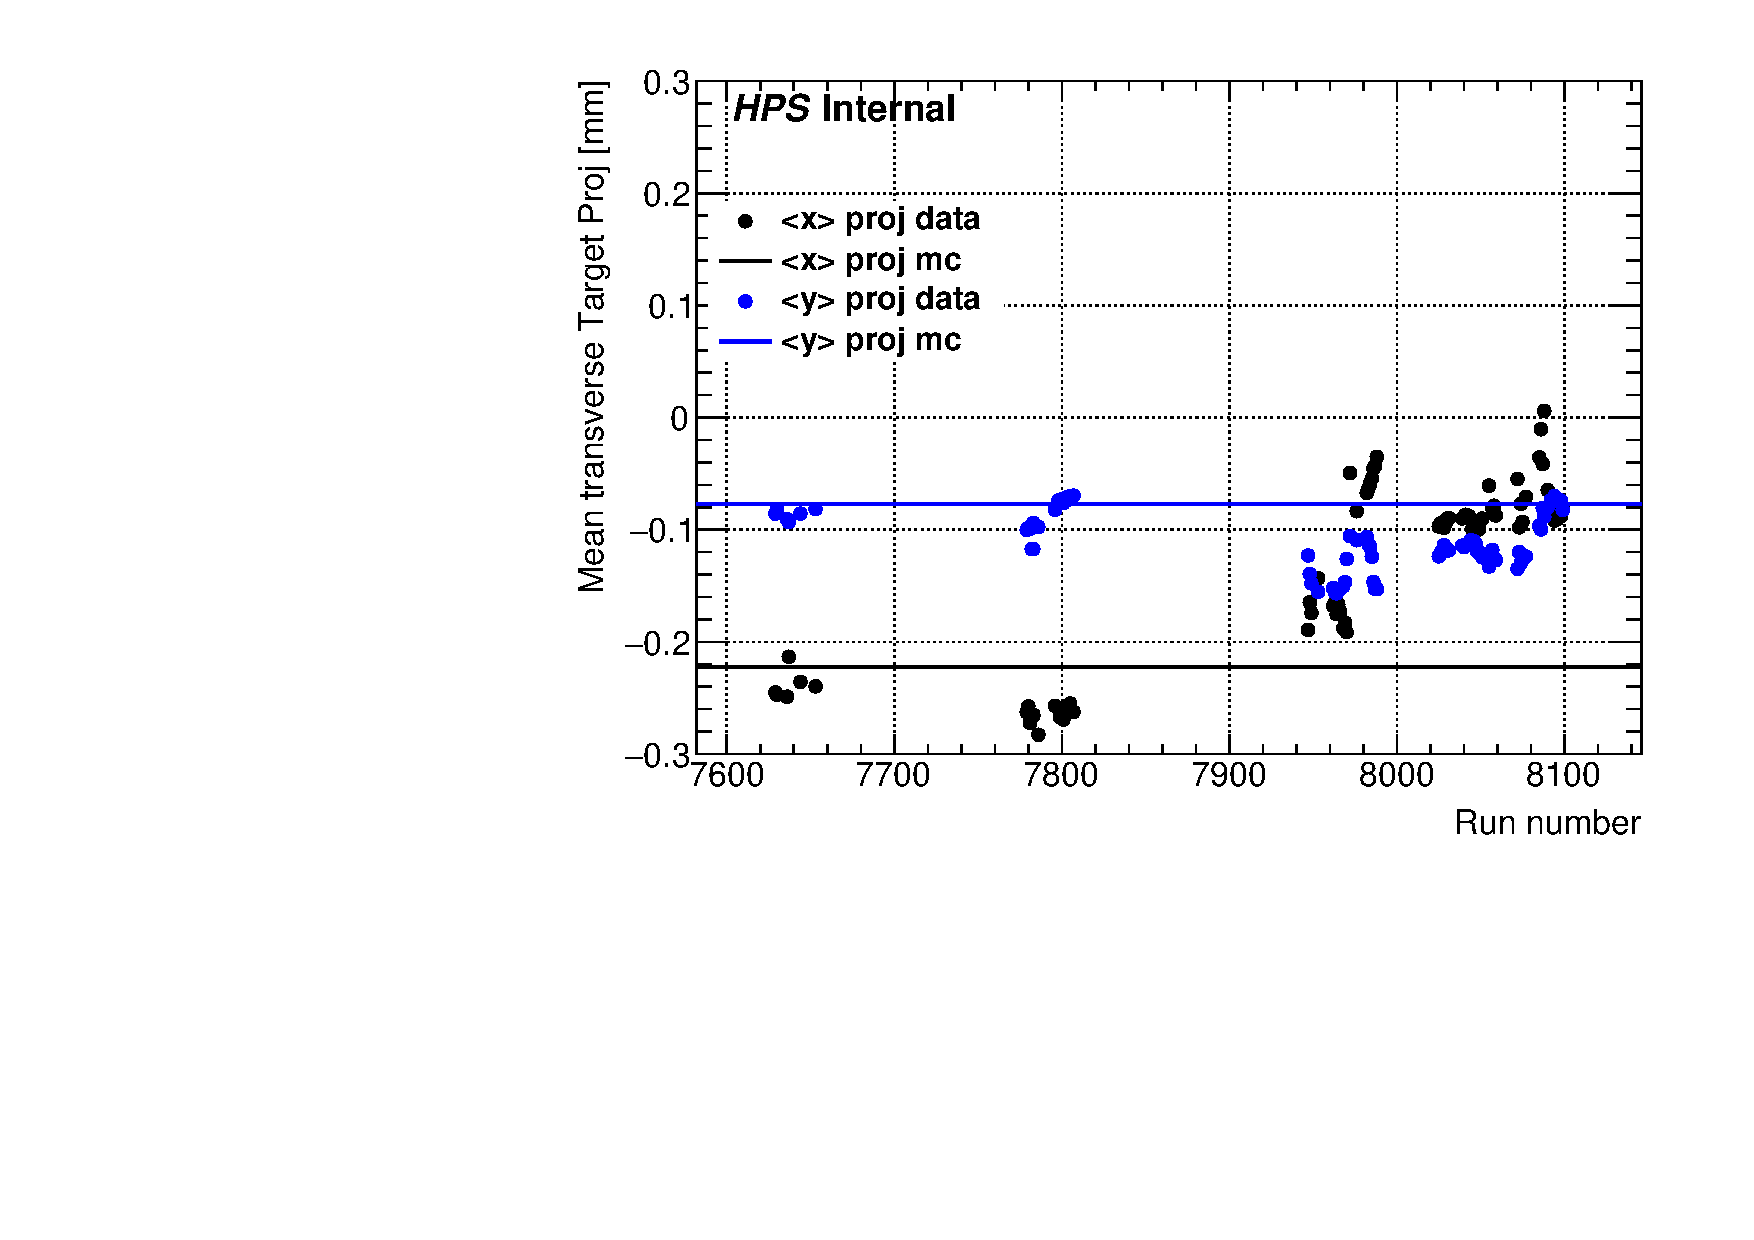
\includegraphics[width=.45\textwidth]{figs/recon/xy_proj_final.pdf}
    %    \caption{}
    %\end{subfigure}
    \caption{%The run-dependent average position in $x$ and $y$ for unconstrained vertices fit (a) and target projections (b) represented by solid points and a solid line for data and MC simulation, respectively.
    The run-dependent mean (left) and width (right) in $x$ and $y$ for the unconstrained vertex position in data. The MC is represented as a solid line.}
    \label{fig:rundepposxy}
\end{figure*}


%\begin{figure*}[t!]
%    \centering
    %\begin{subfigure}[t]{0.45\textwidth}
    %    \centering
%        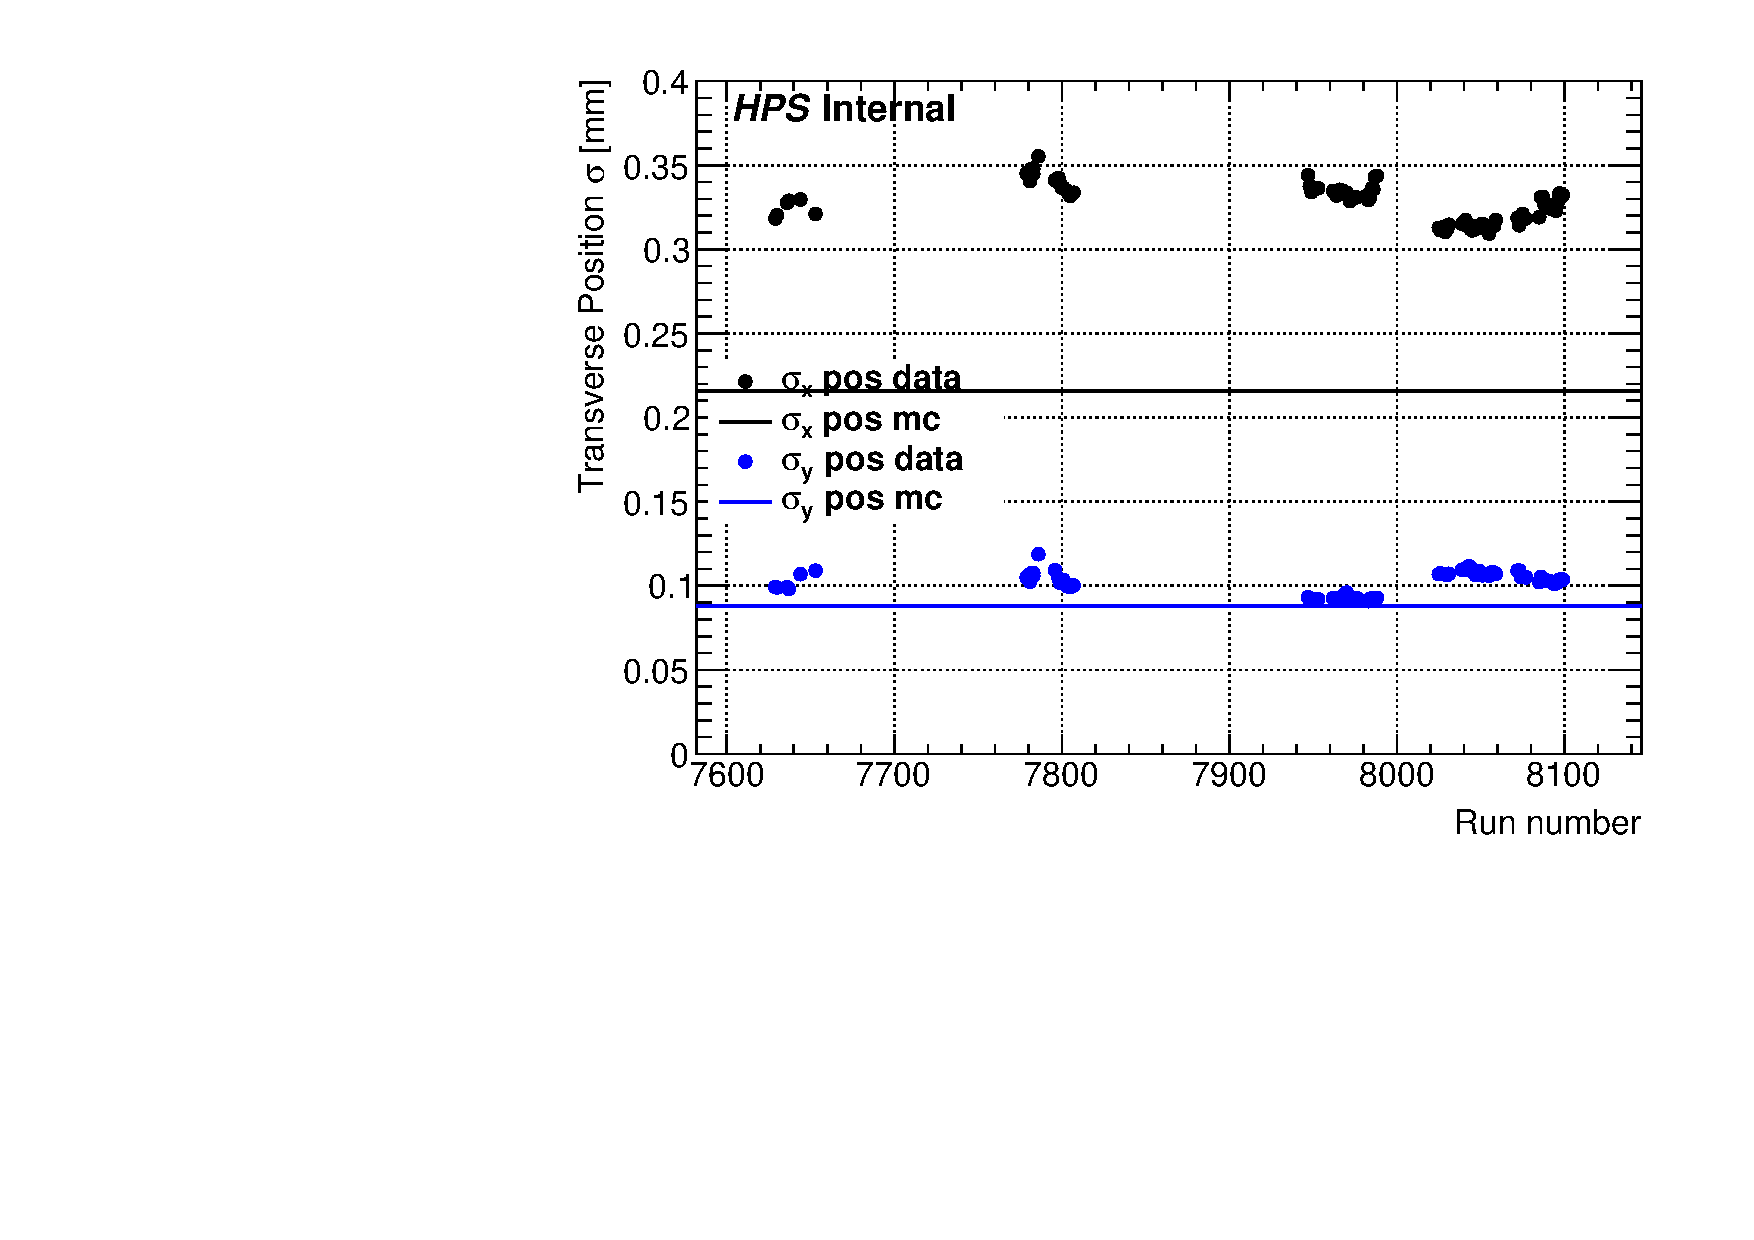
\includegraphics[width=.45\textwidth]{figs/recon/sigma_xy_final.pdf}
    %\caption{}
    %\end{subfigure}%
    %~ 
    %\begin{subfigure}[t]{0.45\textwidth}
    %    \centering
%        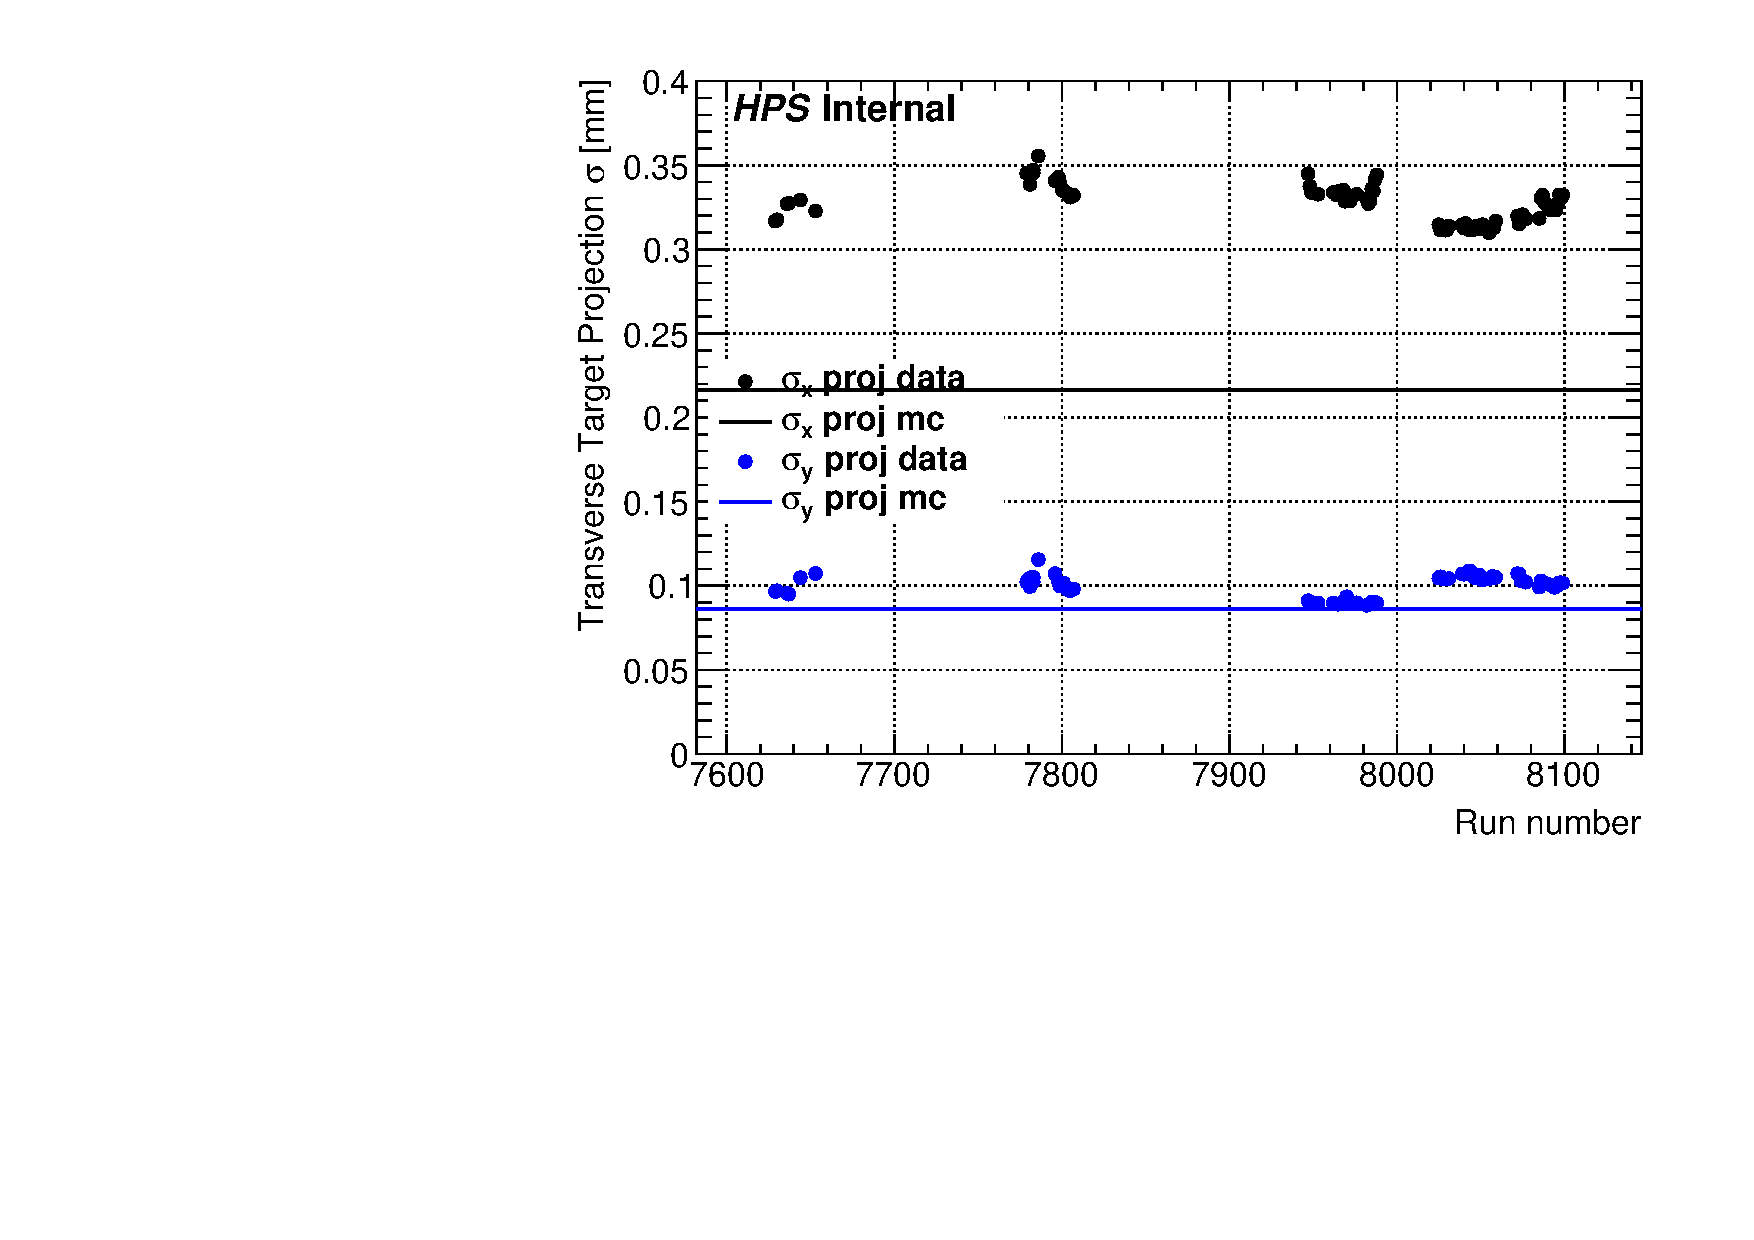
\includegraphics[width=.45\textwidth]{figs/recon/sigma_xy_proj_final.pdf}
    %    \caption{}
    %\end{subfigure}
%    \caption{The run-dependent mean (left) and width (right) in $x$ and $y$ for the unconstrained vertex position in data.}
%    \label{fig:rundepposxys}
%\end{figure*}

\clearpage

\section{Hit Efficiency}\label{sec:hiteff}

\begin{figure}[t]
    \centering
    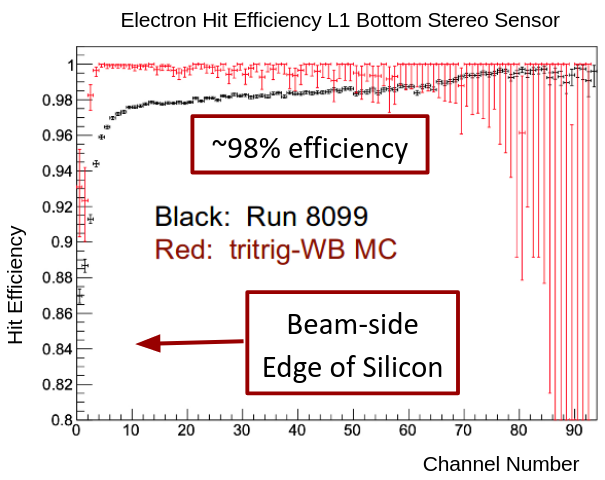
\includegraphics[width=.85\textwidth]{figs/recon/hiteff.png}
    %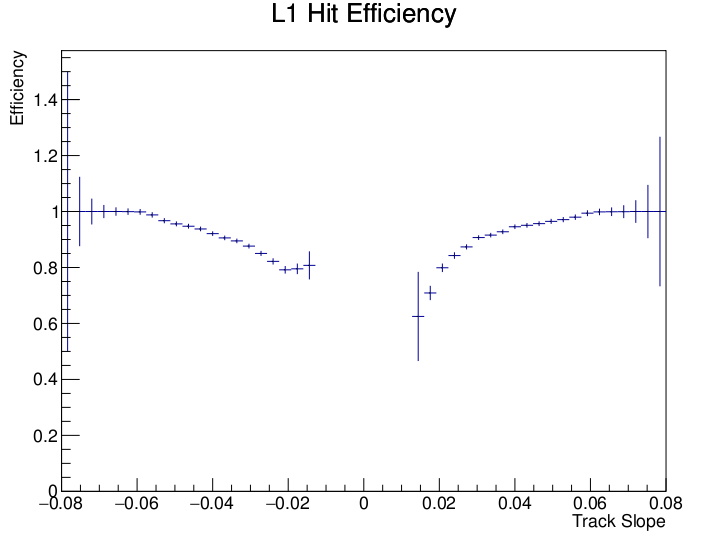
\includegraphics[width=.45\textwidth]{figs/recon/L1_eff.png}
    \caption{The measured SVT layer 1 efficiency for electrons in layer 1 bottom stereo sensor. The MC does not have the correct hit efficiencies. %Right: The layer 1 hit efficiency as a function of track slope (tan$\lambda$) used for the hit killing algorithm described in Sec \textcolor{red}{Section}.\textcolor{red}{Replace these figures. Add a positron hit efficiency plot.}}
    }
    \label{fig:L1eff}
\end{figure}

%It is useful to know the hit efficiency. In principle we should account for multiple scattering effects; however, our errors are wrong. This becomes the basis for unbiased hit residuals, which are useful for tracker alignment. 

The HPS detector has hit efficiency effects that must be properly accounted for, particularly in the first layer of the SVT where occupancies are significantly higher than the other layers of the tracker. The main source of hit inefficiencies are wide angle bremsstrahlung conversions (WABs) in layer 1 of the SVT. Positrons from converted WABs are less likely to deposit sufficient energy into a silicon strip to pass readout threshold. This could result in a track that extrapolates to the active area of a layer 1 sensor that lacks a reconstructed hit, and thus will appear as a hit inefficiency in the method described below. This can be seen in a comparison of the hit efficiencies in layer 1 for positrons and electrons in Fig. \ref{fig:L1_eff} where the difference in efficiency between electrons and positrons can be attributed to converted WABs. 

The remaining sources of hit inefficiencies are mostly unknown and are still under exploration. One hypothesis is some of the channels are readout, but the corresponding waveforms fail the fit requirements of the hit reconstruction stage described in Sec. \ref{sec:svtrecon}. There is evidence of this from the fact that layer 1 hit inefficiencies occur at the strips nearest to the beam plane which have the highest occupancies due to elastically-scattered beam in the target and x-ray emissions from the target.

Hit efficiencies are measured using a track refit to a layer of interest, and an unbiased extrapolation to that layer to see if a hit lies within a certain window of the extrapolated position. As an example, in order to measure layer 1 efficiencies, the standard track reconstruction is performed on all layers except for layer 1. The tracks that meet basic quality requirements are extrapolated to both the axial and stereo sensor planes in layer 1. For the tracks that extrapolate to the active area of the sensor of interest, if a 1D hit is not found within 5$\sigma$ of the extrapolation error it is counted as a hit inefficiency. The hit efficiency is defined as the ratio of the number of tracks with a hit within the defined extrapolation window to the total number of tracks sampled.  

Due to the highly non-uniform nature of occupancies on the sensors, the hit inefficiencies are studied in each sensor as a function of the extrapolated track position on the sensor. %\footnote{The extrapolated track must be used since, for an inefficiency, one cannot assign an inefficiency to a specific channel.}
A sample of measured hit efficiency in data in comparison with MC as a function of channel number for the layer 1 bottom stereo sensor is shown in Fig. \ref{fig:L1eff}. In addition, there are multiple scattering effects that result in a reduced measured hit efficiency on the edge of the sensors due to the fact that particle trajectories that don't traverse the active sensor area reconstruct a track that extrapolates to the active sensor area due to resolution effects (and thus counted as a hit inefficiency). This is most visible in MC which does not contain any hit efficiencies yet has a rapidly decreasing measured hit efficiency along the edge of the sensor. In principle, this can be corrected if errors on track extrapolations are computed correctly.

Unfortunately hit efficiencies are not present in the MC, and methods of incorporating these effects are under investigation. However, hit efficiencies will affect the signal rate and distributions for a variety of variables of interest. To account for hit efficiencies in both a simple and reasonable way, a post-reconstruction hit killing algorithm based on track slope is applied to signal MC (and some background distributions). This method is described in detail in Sec. \ref{sec:hitkill}. 

%As an example, in order to measure layer 1 efficiencies, the layer 1 hit of a track is removed and the track is refit using the remaining hits (). Then, the refit track is extrapolated to both axial and stereo sensors in layer 1. For each sensor, if a 1D hit is found within 5$\sigma$ of the extrapolation error it is counted in the numerator. The hit efficiency is the ratio of the number to the total number of tracks sampled Due to the highly non-linear nature of occupancies on the sensors, the hit efficiencies are separated by channel number using the position of the extrapolated track at each sensor\footnote{The extrapolated track must be used since for an inefficiency, one cannot assign it to a specific channel.}. A sample of measured hit efficiency in data in comparison with MC as a function of channel number for the layer 1 bottom stereo sensor is shown in Fig. \ref{fig:L1_eff}. M.S. effect.

%The HPS detector has hit efficiency effects, particularly in the first layer of the SVT, that must be accounted for in the $A'$ efficiencies. Hit efficiencies are measured using a track refit to a layer of interest, and an unbiased extrapolation to the layer to see if a hit lies withing a certain window. A sample of measured hit efficiency in data in comparison with MC for the layer 1 bottom stereo sensor is shown in Fig. \ref{fig:L1_eff}. %Some sources are known, others are not. The most major source are wide angle bremstrahlung conversions (WABs)in layer 1 of the SVT. This can be seen in a comparison of the hit efficiencies in layer 1 for positrons and electrons in Fig. (?). Positrons from converted WABs are less likely to leave a hit in the silicon, and will appear as a hit inefficiency in the method above. Thus, the difference in efficiency between electrons and positrons can be attributed to converted WABs.


%Unfortunately hit efficiencies are not present in the MC, and methods of incorporating these effects are under investigation. However, this effect that will affect the signal rate and distributions. To account for hit efficiencies in both a simple and reasonable way, a post-reconstruction hit killing algorithm based on track slope is applied to signal MC (and some background distributions \textcolor{red}{and L1L2}). This method is described in detail in Sec. \textcolor{red}{Section}. %as a function of track slope shown in in Fig. \ref{fig:L1_eff}. %If a track passes the hit killing algorithm, nothing changes. However, if a track fails the hit killing algorithm, the layer 1 hit is removed and the $A'$ can either migrate into another category or be eliminated. Details on what happens to an $A'$ with the hit killing algorithm is as follows:

\clearpage

\section{Tracker Alignment}\label{sec:alignment}

%\begin{figure}[t]
%    \centering
%    
\includegraphics[width=.35\textwidth]{figs/placeholder.jpg}
%    
\includegraphics[width=.35\textwidth]{figs/placeholder.jpg}
%    \caption{The target position is found to be -4.3 mm. \textcolor{red}{I actually need to get these plots. Some placeholders are there for now.}}
%    \label{fig:truth_match}
%\end{figure}

An initial mechanical survey is applied to the SVT as described in Sec. \ref{sec:svt_mechanical} which defines sensor positions with a precision of 50 - 100 $\mu$m. This level of imprecision will create systematic shifts in track parameters and artificially degrade tracking and vertexing resolutions, thus is insufficient to meet the HPS physics goals. In order to mitigate alignment-related effects, an offline alignment using particle trajectories to find the sensor positions and orientations as close as possible to their true values is performed.

Detector alignment comes in two steps - internal alignment and global alignment. The internal alignment finds the sensor positions relative to each other using the top and bottom volumes of the SVT separately with the goal of minimizing the track $\chi^2$. The internal alignment utilizes Millepede-II which was developed for fast alignment of large tracking detectors such as CMS \cite{BLOBEL20065} \cite{BLOBEL20111760}. Each sensor can be corrected by translation along or rotation about the three coordinate axis for a total of six possible alignment corrections.

These corrections are not equally important. For instance, track parameters are sensitive to translations along the measurement direction in a given sensor but completely insensitive to translations along the non-measurement direction (other than minor acceptance affects for tracks on the sensor edge). For simplicity, only translations along the measurement direction and beam direction as well as rotations about the sensor normal were considered. The sensor position and orientations were found by iterating with different alignment configurations that float a single sensor position or orientation until the optimal alignment constant is found.

Global alignment involves fixing the so-called ``weak modes'' where sensors move coherently in such a way that the track parameters and track quality are unaffected. Since there are 5 track parameters there are 5 weak modes - translating in the horizontal ($d0$) and vertical directions ($z0$), rotating tracks horizontally ($\phi$) and vertically (tan$\lambda$), and the horizontal quadratic shear ($\Omega$).

Elastically-scattered electrons from the target ($e^-Z \rightarrow e^-Z$) have a known momentum at the beam energy, a known origin at the beam spot on the target, and sufficiently populate the full HPS angular acceptance making them ideal to study various weak modes. First the known curvature, provides a way to study the horizontal quadratic shear. Second, the known origin provides a way to study the translational weak modes as well as the $z$ position of the target $z_{targ}$. In the $yz$-plane the extrapolated $y$ position of any track can be parametrized as follows:

\begin{equation}
    y(z) = y_{beam} + \mathrm{tan} \lambda \times (z - z_{targ})
    \label{eqn:alignment}
\end{equation}

where tan$\lambda$ is the track slope defined in Sec. \ref{sec:coordinates}. The equation contains two unknowns - the target position in $z$ and the beam position in $y_{beam}$. This can be resolved by using both the top and bottom halves of the SVT by moving in the vertical direction until their measurements are in agreement. From this, the target position is determined, and for the 2016 Engineering Run the target is measured to be at a $z$-position of -4.3 mm relative to the origin in detector coordinates. Similarly, the x position of the beamspot $x_{beam}$ can be found using the same method. %\textcolor{red}{Include the target position.}

M\o ller-scattered electron pairs, that is beam electrons that scatter off of a target electron, have a known momentum equal to the momentum of the beam, including both magnitude and direction. This can be used to measure the beam angle deviation from the nominal beam axis. In addition, the two-body kinematics of M\o ller scattering is identical to Compton scattering and has the following relation:

\begin{equation}
    m_ec^2 \left( 1/E - 1/E_{beam} \right) = 1 - \mathrm{cos} \ \theta
    \label{eqn:moller}
\end{equation}

where $\theta$ is the angle from the beam axis and $E$ is the energy of the $e^-e^-$ pair. As a result, all M\o llers at a specific energy will scatter at the same angle from the beam axis which can be used to constrain both the rotational weak modes. M\o ller-scattered electrons are also useful as a ``standard candle'' for determining the mass scale and mass resolution as described in Sec. \ref{sec:massresolution}.

\clearpage

\section{Track-Truth Matching}\label{sec:tracktruth}

\begin{figure}[t]
    \centering
    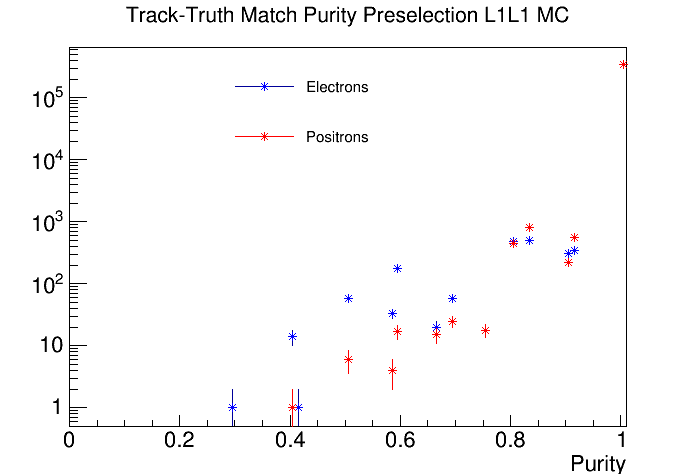
\includegraphics[width=.45\textwidth]{figs/recon/purity.png}
    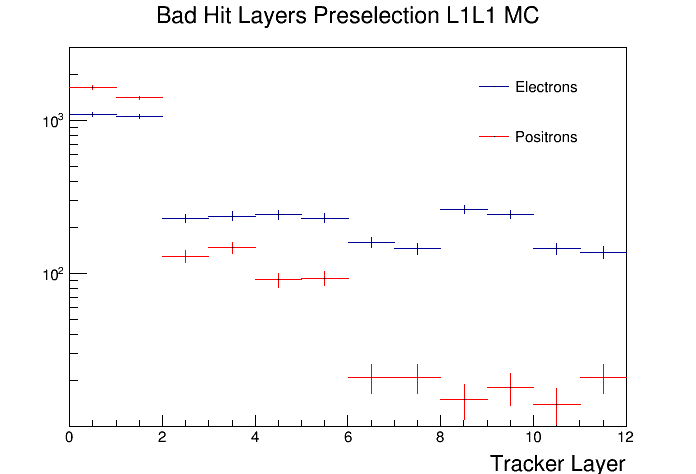
\includegraphics[width=.45\textwidth]{figs/recon/badhit_layers.png}
    \caption{Left: The purity for $\epem$ tracks with preselection and layer 1 requirements for tritrig-wab-beam MC. Purity is a measure of the fraction of hits on track that are associated with the truth-matched particle. Right: Tracking layers (ordered in sensor number from upstream to downstream) that contain a hit on track not associated with the truth particle matched to the track (i.e. a bad hit).}
    \label{fig:truth_match}
\end{figure}

%Due to the nature of backgrounds due to mistracking as described in Sec \textcolor{red}{Section}, it is useful in the displaced vertex search for tracks to be matched to truth particles in the MC. 
In order to study backgrounds resulting from tracking errors, it is useful in the MC to match tracks with the particles that generated them, and study which tracks have incorrectly included errant hits (referred to as mis-tracking). This will enable a detailed study of mis-tracked backgrounds that can falsely reconstruct downstream of the target and appear signal-like. A simple track-truth matching algorithm is performed after reconstruction, and the algorithm is as follows:

%order for a detailed understand for certain types of backgrounds (like those due to mistracking described in the Isolation Cut section). A simple track-truth matching algorithm is performed after reconstruction. In the reconstruction process, the tracker hits are mapped to MCParticles and tracks are mapped to tracker hits. The track-truth matching algorithm is as follows:

\begin{enumerate}
  \item In the reconstruction process, the hits on track (i.e. the tracker hits) are each mapped to a list of truth particles (called MCParticles) that contribute to the hit.
  \item For each MCParticle, the number of tracker hits associated with a given track is tabulated.
  \item The MCParticle with the highest score, that is the highest number of tracker hits on a given track, is considered to be the truth match.
  \item If there is a tie in this score, the MCParticle with the inner most hits (closer to the target) is considered the to be the truth match. More precisely, a loop is performed over the tracker hits in order from first sensor to last sensor, and the MCParticle that does not contribute to a tracker hit first in this loop is no longer considered for the truth match.
  \item If there is still a tie, the higher momentum MCParticle is considered to be the truth match. This last tie breaker is arbitrary and its occurrence is exceedingly rare, if ever.
\end{enumerate}

%The MCParticle with the highest score (highest number of hits that contribute to the 1D hits on track) is the labeled as the ``truth match''. If there is a tie in the scored, the MCParticle with the inner most hits is considered the truth match. More precisely, if you loop through the hits on track in order from first layer to last layer, the MCParticle with that does not contribute to a tracker hit first in the loop is no longer considered for the truth match. If there is still a tie (which is very rare if ever), the higher momentum MCParticle is selected as the truth match.

Once an MCParticle is matched to a track, the quality of the match can be quantified by computing the purity of the match - which is defined as the ratio of hits the truth-matched MC particle contributes to the track to the total number of hits on track (a fraction of 10 for 5-hit tracks and a fraction of 12 for 6-hit tracks). The purity of the preselection with layer one requirements of tritrig-wab-beam for positrons and electrons is shown in Fig. \ref{fig:truth_match}. In this sample, about 0.002\% of $e^+$ and $e^-$ tracks do not have a MCParticle match to a track where the most likely explanation are particles with truth information that is not propagated to the reconstruction level. These truth-matched tracks are used to study backgrounds due to mistracking in detail.

\clearpage

\section{Monte Carlo Samples}\label{sec:mc}

\begin{table}[!hb] 
\centering
\begin{tabular}{ccc}
   \toprule    
    Sample & Generator & Statistics \\
    \midrule
     RAD      & MadGraph5 & $\sim$2.9M \\
     Tritrig & MadGraph5 & $\sim$8.0M \\
     WABs     & MadGraph4 & $\sim$32k \\
     A$^{'}$ prompt & MadGraph4 & $\sim$3.8M \\
     A$^{'}$ displaced & MadGraph4 & $\sim$56k \\
     M\o ller & EGS5 & $\sim$500k \\
     Beam & EGS5 & -- \\   
     \bottomrule
\end{tabular}
\caption{Event generators and statistics for MC samples.}
\label{table:samples}
\end{table}

In order to be confident that the results from the analysis are well-understood, realistic Monte Carlo (MC) samples are run for particular physics processes. %Specifically for the physics background studies, we are most interested in correctly simulating trident physics processes and converted bremsstrahlung as well as multiple and single Coulomb scattering of particles in the tracker. Both prompt and displaced $A'$s are also simulated for signal kinematics.
It is important to properly simulate all the physics processes that make up an appreciable fraction of the triggered data. The main $\epem$ physics backgrounds are tridents composed of radiatives (RAD), Bethe-Heitler (BH), and their cross terms as described in Sec. \ref{sec:backgrounds} as well as converted wide-angle bremsstrahlung (cWABs). WABs are the dominant triggered process since charged particles are not required in the trigger. M\o ller scattering occurs when a beam electron scatters off a target electron. This provides a useful ``standard candle'' for the mass scale and mass resolution as described in Sec. \ref{sec:alignment}, thus a comparison between data and MC is necessary. Lastly, backgrounds from beam electrons which have elastically scattered in the target are present in the triggered data in large quantities. Even though a simple selection of a maximum electron momentum eliminates beam particles, beam particles can leave hits in the tracker and significantly affect the pattern recognition and track reconstruction. Thus, beam backgrounds need to be understood in detail, and all processes are overlaid with beam background.

For event generation and cross-section computation, the HPS MC chain uses several generators depending on the specific physics process of interest including EGS5 \cite{hirayama2005egs5} and MadGraph4 \cite{Alwall_2007}. Trident processes, wide-angle bremsstrahlung (WABs), and $A'$s are generated using MadGraph4. The Feynman diagrams are shown in Fig. \ref{fig:feynman-diagram}. Beam background, M\o llers, and scattering in the target are simulated using EGS5. All prompt processes are passed through EGS5 to properly simulate the scattering in the target which produces EGS5 final state particles. From EGS5 final state particles, a package called Stdhep is used to persist truth information and build beam bunches using a Poisson distribution as well as account for the the beam size, orientation, and offset. %and build beam bunches using a Poisson distribution for beam backgrounds.

The detector response is then simulated using a GEANT4-based package called Slic (Simulator for the Linear Collider) \cite{doi:10.1063/1.2396991}. The detector response, specifically for the SVT and the Ecal, is converted into raw hits with time stamps and energy deposition information.

\begin{figure}[!h]
    \centering
    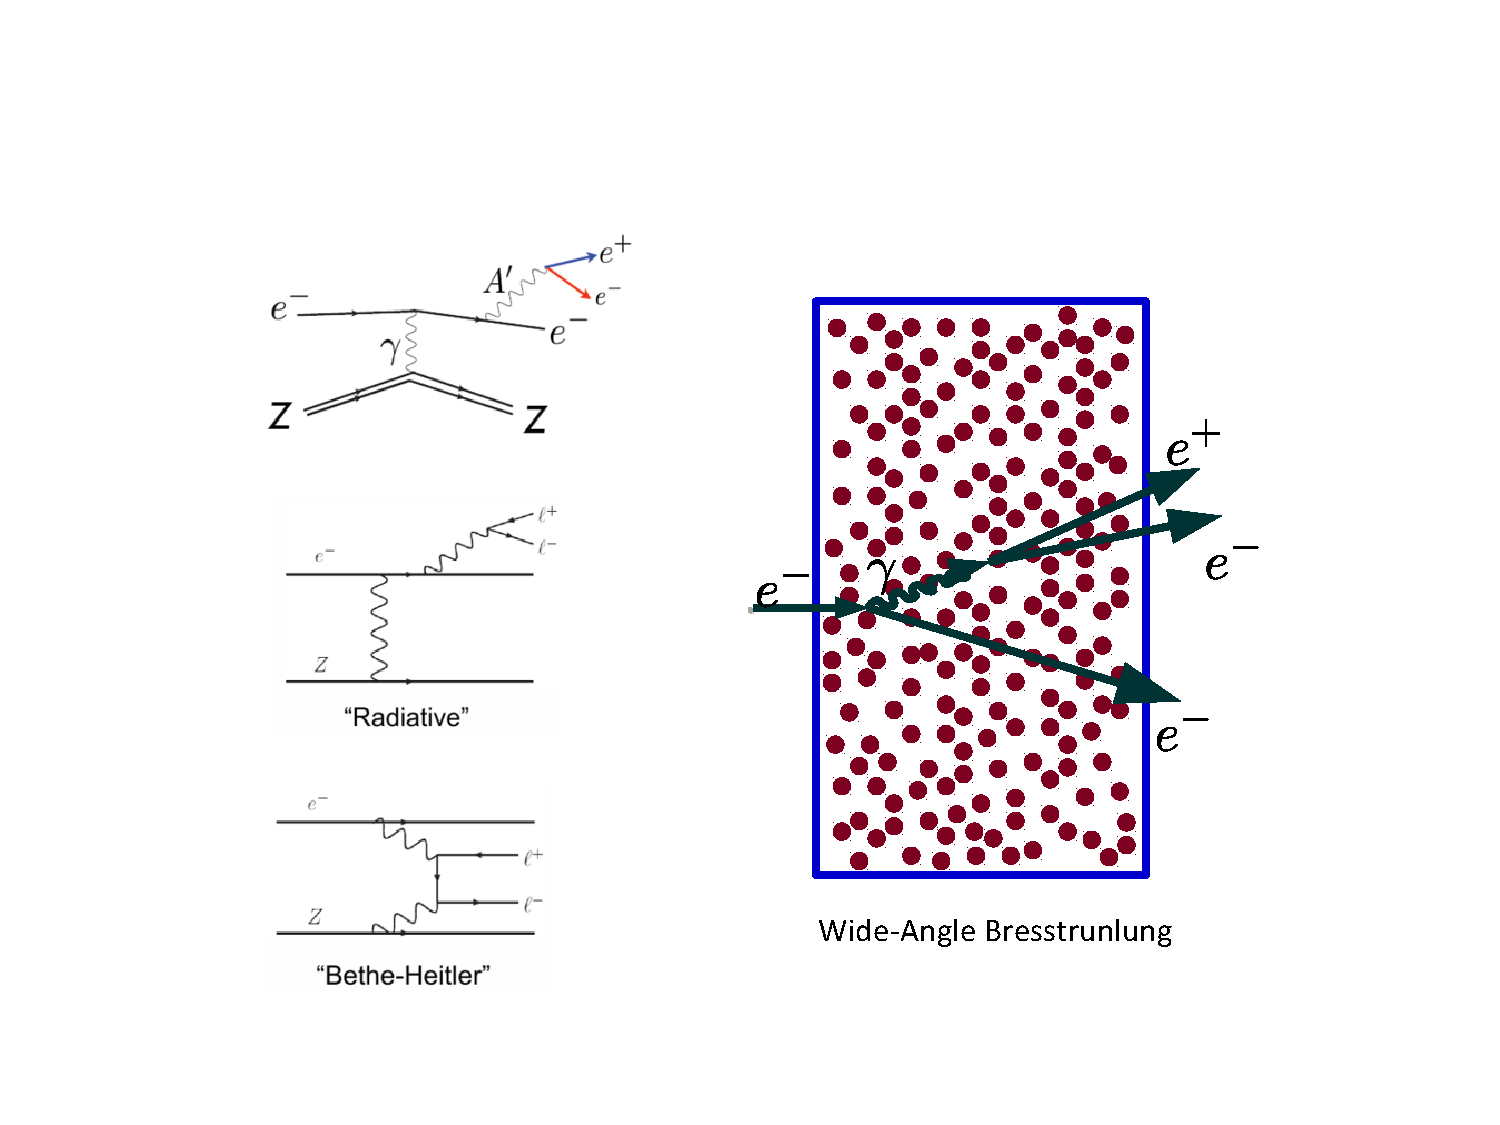
\includegraphics[width=1.\textwidth]{figs/recon/feynman-diagram.pdf}
    \caption{Left pictures show Feynman diagrams for A$^{'}$ (top), RAD (middle) and BH (bottom) events. Right picture shows WAB process.}
    \label{fig:feynman-diagram}
\end{figure}

Next, the raw hit information must pass through the readout simulation which emulates the trigger response including digitization and readout. Finally, the digitization from the readout simulation is used as input in the physics reconstruction software in hps-java in the same way the real experimental data is reconstructed. This provides a way for data and simulation to be directly compared, with MC able to be separated into different background components.

The MC samples produced as shown in Table \ref{table:samples} are background samples of RAD, tritrig, WAB, M\o ller, and beam background. The $A'$ samples come in two different types - prompt and displaced from the target. Prompt $A'$ samples are used for the resonance search and for an estimate of the mass resolution described in Sec. \ref{sec:massresolution} (mass resolution is independent of displacement). The displaced $A'$s are used to estimate the $z$-dependence of efficiency and geometrical acceptance. The detailed generator level requirements for each MC sample are shown in Table \ref{table:MCrequirements}.

Both prompt and displaced $\aprime$ samples are generated at specific mass points over the range of interest determined by the acceptance at a specific beam energy, and with close enough spacing such that interpolation of acceptance between mass points contains minimal error. The mass points generated are between 50 MeV and 150 MeV in increments of 5 MeV as well as a high mass point at 175 MeV. The displaced $\aprime$ samples must populate the decay range of interest ($\sim 0-150$ mm) with sufficient statistics. These samples are produced with a constant livetime at $c\tau=10$ mm, which is large enough to sufficiently populate the decay range of interest for HPS, and then reweighted at a later step to reflect actual signal shapes.

\begin{table}[!hb] 
\centering
\begin{tabular}{llc}
   \toprule    
    Sample & Cut Description & Cut Requirement  \\
    \midrule
     RAD & Min energy of daughter particles & $E_{e^+}>50$ MeV and $E_{e^-}>50$ MeV \\
     RAD & Min for $y$-direction of $\epem$ particles & $p_{e^+,y}/p_{e^+}>0.005$ and $p_{e^-,y}/p_{e^-}>0.005$ \\
     RAD & Min total energy of $\epem$ pair & $E_{e^+}+E_{e^-}>500$ MeV \\
     RAD & Min invariant mass of $\epem$ pair& $m_{e^+e^-}>10$ MeV \\
     \midrule
     \midrule
     Tritrig & Min energy of $e^+$ & $E_{e^+}>100$ MeV \\
     Tritrig & Min for $y$-direction of $e^+$& $p_{e^+,y}/p_{e^+}>0.005$ \\
     Tritrig & Min total energy of a $\epem$ pair & $E_{e^+}+E_{e^-}>1000$ MeV \\
     Tritrig & Min invariant mass of a $\epem$ pair & $m_{e^+e^-}>10$ MeV \\
     \midrule
     \midrule
     WABs & Min photon energy & $E_{\gamma}>400$ MeV \\
     WABs & Min for $y$-direction of $\epem$ particles & $p_{\gamma,y}/p_{\gamma}>0.005$ \\
     \midrule
     \midrule
     M\o ller & Min energy of final state particles & $E>10$ MeV \\
     M\o ller & Min for transverse direction for f.s. particles & $\sqrt{(p_x/p)^2+(p_y/p)^2}>0.005$ \\
     \midrule
     \midrule
     Beam & Min energy of beam particles & $E_{e^-}>0.005E_{beam}$ \\
     Beam & Min for transverse direction for f.s. particles & $\sqrt{(p_x/p)^2+(p_y/p)^2}>0.005$ \\
     \midrule
     \midrule
     Photon & Min for $y$-direction of $\gamma$ & $p_{\gamma,y}/p_{\gamma}>0.004$\\
     Photon & Max for $y$-direction of $\gamma$ & $p_{\gamma,y}/p_{\gamma}<0.005$\\
     \midrule
     \midrule
     $A'$s Prompt & None & -- \\
     $A'$s Displaced & None & -- \\
     \bottomrule
\end{tabular}
\caption{Basic generator level physics requirements for different physics processes. $\aprime$s have no generator level cuts since knowledge of the geometrical acceptance is required to compute the expected number of $\aprime$s for different mass and $\epsilon$ values.}
\label{table:MCrequirements}
\end{table}

Detailed steps on the production of beam particles are as follows:
\begin{enumerate}
  \item Beam particles are produced in EGS5.
  \item Beam rotation, beam size, and the target offset are all applied via stdhep. Beam particles are sampled and beam bunches are built in stdhep.
  \item The beam bunches are passed through Slic.
\end{enumerate}

Detailed steps on the remaining MC - RAD, tritrig, WAB, M\o llers, and $A'$ with beam overlay - are as follows:
\begin{enumerate}
  \item Particles are produced in MadGraph. The exception is that M\o llers are produced in EGS5.
  \item Final state particles from MadGraph are passed through the target via EGS5. Because displaced $\aprime$ have no interaction with the target, only the recoil electron for these samples is passed through the target.
  \item Parent particles are added into each event of the EGS5 output.
  \item Beam rotation, beam size, and the target offset are all applied via stdhep. 
  \item The events are passed through Slic.
  \item The output events from Slic are spaced apart by a fixed interval equal to the event window size in the trigger system.
  \item The sample is mixed with the beam sample or a WAB sample if desired.
  \item Readout and reconstruction is processed.
\end{enumerate}

Lastly, since the displaced vertex analysis is mostly concerned with a near-zero background region far beyond the target, the background shapes at the extreme tails of the reconstructed $z$ distributions must be understood. In order to do this, a sample of tridents overlaid with beam and WABs, with the trident luminosity equivalent to the luminosity of the dataset, is generated. This gives some indication of the high $z$ background due to both mis-tracking and large scatterings in the tracker and is used as a direct comparison to data in Chapter \ref{chap:aprimes}.

In addition, a sample of pure tridents with about three times the luminosity in data is used to further understand the tails of the $z$ distributions due to prompt processes that undergo significant multiple scattering or single Coulomb scattering and reconstruct far downstream of the target. The pure trident sample is used for the high luminosity sample because overlaying a sample with beam is computationally expensive.

\clearpage

\section{$\epem$ Preselection}\label{sec:preselection}

After reconstruction, analysis can be performed. The goal of the displaced vertex analysis is to search for long-lived $A'$s produced in a fixed target that decay to $\epem$ pairs in the range $\sim 1-10$ cm in the lab frame. These rare signal processes must be distinguished from a large number of prompt QED tridents, and this search is limited by the vertex resolution of HPS and the quality of tracking. In this energy range, the vertex resolution is dominated by multiple scattering in the tracker, particularly in the first layer. In order to perform the search most effectively, a series of analysis cuts are utilized to separate the prompt background that reconstructs falsely downstream of the target from true long-lived particles. Because the expected relative signal rate is very low, a near-zero background region is required to make this search possible. Thus, these cuts aimed to eliminate nearly all background in a signal region that is sufficiently downstream of the target without sacrificing too much signal efficiency.

%%%%%%%%%%%%%%%%%%%%%%%%%%%%%%%%%%%%%%%%%
%   Table: Preprocessing requirements   %
%%%%%%%%%%%%%%%%%%%%%%%%%%%%%%%%%%%%%%%%%

%Many of the selection cuts are shared with the resonance search selection or were studied in the previous displaced vertex analysis from the 2015 Engineering Run. The physics trigger used by HPS was tuned to accept time coincident $\epem$ pairs, where the $e^+$ and $\ele$ reside in opposite detector volumes. Therefore, as an initial requirement, the Ecal clusters associated with the $e^+$ and $\ele$ are required to be in opposite halves of the detector, i.e. have a $y$ position which satisfies the following relation:
%\begin{equation}
%  y_{\e^+ \text{ Cluster}} \times y_{\ele\text{ Cluster}} < 0.
%\end{equation}

%In addition, several loose cuts are required at the reconstruction stage, the so-called pre-processing cuts which are shown in Table \ref{tab:mouse_data} for data and Table \ref{tab:mouse_mc} for MC. 
%Since this analysis only considers pairs formed using tracks that are matched to Ecal clusters, a loose cut is placed on the track-cluster matching $\chi^2$ to guard against the case where a track is grossly mismatched to an Ecal cluster. To further reduce those events, a loose cut is placed on the time difference between $\epem$ clusters and the time difference between the track and the matched cluster to eliminate out of time events. In addition, we require a loose track quality. Finally, we place a loose cut on the maximum electron momentum to further reduce elastically scattered electrons in the target and on the maximum V0 momentum. Each of these MOUSE cuts - cluster-track time difference, cluster time difference, track-cluster matching, electron momentum, track quality, and momentum V0 cut - will have a tighter cut at the Preselection stage.

%\clearpage

\begin{table}[t] 
    \centering
    \begin{tabular}{lr}
        \toprule
        \textbf{Cut Description} & \textbf{Requirement} \\
        \midrule
        Trigger & Pair1 \\
        Track-cluster match & $\chi^2 < 10$  \\
        Cluster Time Difference & $|t_{e^+ Cluster}-t_{e^- Cluster}|<1.45$ ns \\
        Track-Cluster Time Difference & $|t_{e^+ Track}-t_{e^+ Cluster} -$ offset$| < 4$ ns \\
        Track-Cluster Time Difference & $|t_{e^- Track}-t_{e^- Cluster} -$ offset$| < 4$ ns \\
        Beam electron cut & $p(e^{-}) < 1.75$ GeV \\
        Track Quality & $\chi^2/dof < 6$ \\
        Vertex Quality & $\chi^2_{unc} < 10$ \\ 
        Minimum $e^+$ Momentum & $p(e^+)>0.4$ GeV \\
        Minimum $e^-$ Momentum & $p(e^-)>0.4$ GeV \\
        Maximum Vertex Momentum & $V_{0p} < 2.4$ GeV \\
        \bottomrule
    \end{tabular}
    \caption{Requirements applied to V0s after reconstruction as an initial set to study. The time offset for data is 56 ns and the time offset for MC is 43 ns. These requirements are referred to as preselection.}
    \label{tab:preselection}
\end{table}

This section presents and describes the cuts from the reconstruction quality requirements to the quality cuts applied to define kinematic regions used for the background normalization and shape correction evaluation and signal selection optimization. The reconstruction is run on V0 skims on the pass 4 dataset - which have at least one V0 candidate in the event (at least one $e^+e^-$ pair in opposite halves of the detector which makes a reasonable quality vertex). The cut flow is separated into three parts - preprocessing selection (shown previously in Table \ref{tab:mouse_data} and Table \ref{tab:mouse_mc}), preselection (described in Table \ref{tab:preselection} and shown later in Fig. \ref{fig:pre_matchChisq} - Fig. \ref{fig:pre_clT_uncChisq2}), and tight selection (described in Chp. \ref{chap:aprimes}) - each successive part contains stricter requirements to further eliminate backgrounds.

%The cuts used to isolate the final $\epem$ invariant mass distribution along 
%with their efficiency for data, trident MC, radiative MC, WAB MC and 30 MeV
%$A'$ events are summarized in Table \ref{tab:sel_eff}.  The effect of each 
%cut on the data $\epem$ invariant mass sample is also shown in Figure 
%\ref{fig:mass_cutflow}. In total, after all cuts, the final sample contains 
%21M events.

The physics trigger used by HPS was tuned to accept time coincident $\epem$ pairs, where the $e^+$ and $\ele$ reside in opposite detector volumes. Therefore, as an initial requirement, the Ecal clusters associated with the $e^+$ and $\ele$ are required to be in opposite halves of the detector, i.e. have a $y$ position which satisfies the following relation:

\begin{equation}
  y_{\e^+ \mathrm{ Cluster}} \times y_{\ele\mathrm{ Cluster}} < 0.
\end{equation}

In addition, several loose cuts were required at the reconstruction stage, the so-called pre-processing cuts which are shown in Table \ref{tab:mouse_data} for data and Table \ref{tab:mouse_mc} for MC. The vertices contained in the events that pass the trigger requirement are selected by a set of cuts, tighter with respect to the reconstruction quality cuts but still loose enough to select signal-like higher-quality vertices with large statistics. This set of cuts is referred to as \textit{Preselection}. Preselected events are used as a way to study trident rates and as a way to study the need for tighter cuts described in Sec. \ref{sec:apvertexcuts}. At this stage only vertices reconstructed by an unconstrained fit are considered. In general, the preselection cuts are shared with the resonance search selection or were studied in the previous displaced vertex analysis from the 2015 Engineering Run. 

The selection starts by requiring that the distance between the tracks and the matched electromagnetic clusters is less than 10$\sigma$, where $\sigma$ is the error associated to the cluster position. This is shown in Fig. \ref{fig:pre_matchChisq}. This requirement guards against the case where a track is grossly mismatched to an Ecal cluster. To further reduce mismatching, the time difference between the calorimeter clusters matched to SVT tracks in opposite hemispheres is required to be less than 1.45 ns (the Hall B bunches are separated by 2 ns) to reduce out of time events. This cut aims to reduce the contamination due to accidentals to less than 1\%, and is studied in detail in the current resonance search \cite{adrian2018search}. The cluster time difference cut is shown in Fig. \ref{fig:pre_clT_uncChisq}.

\begin{figure}[t]
    \centering
    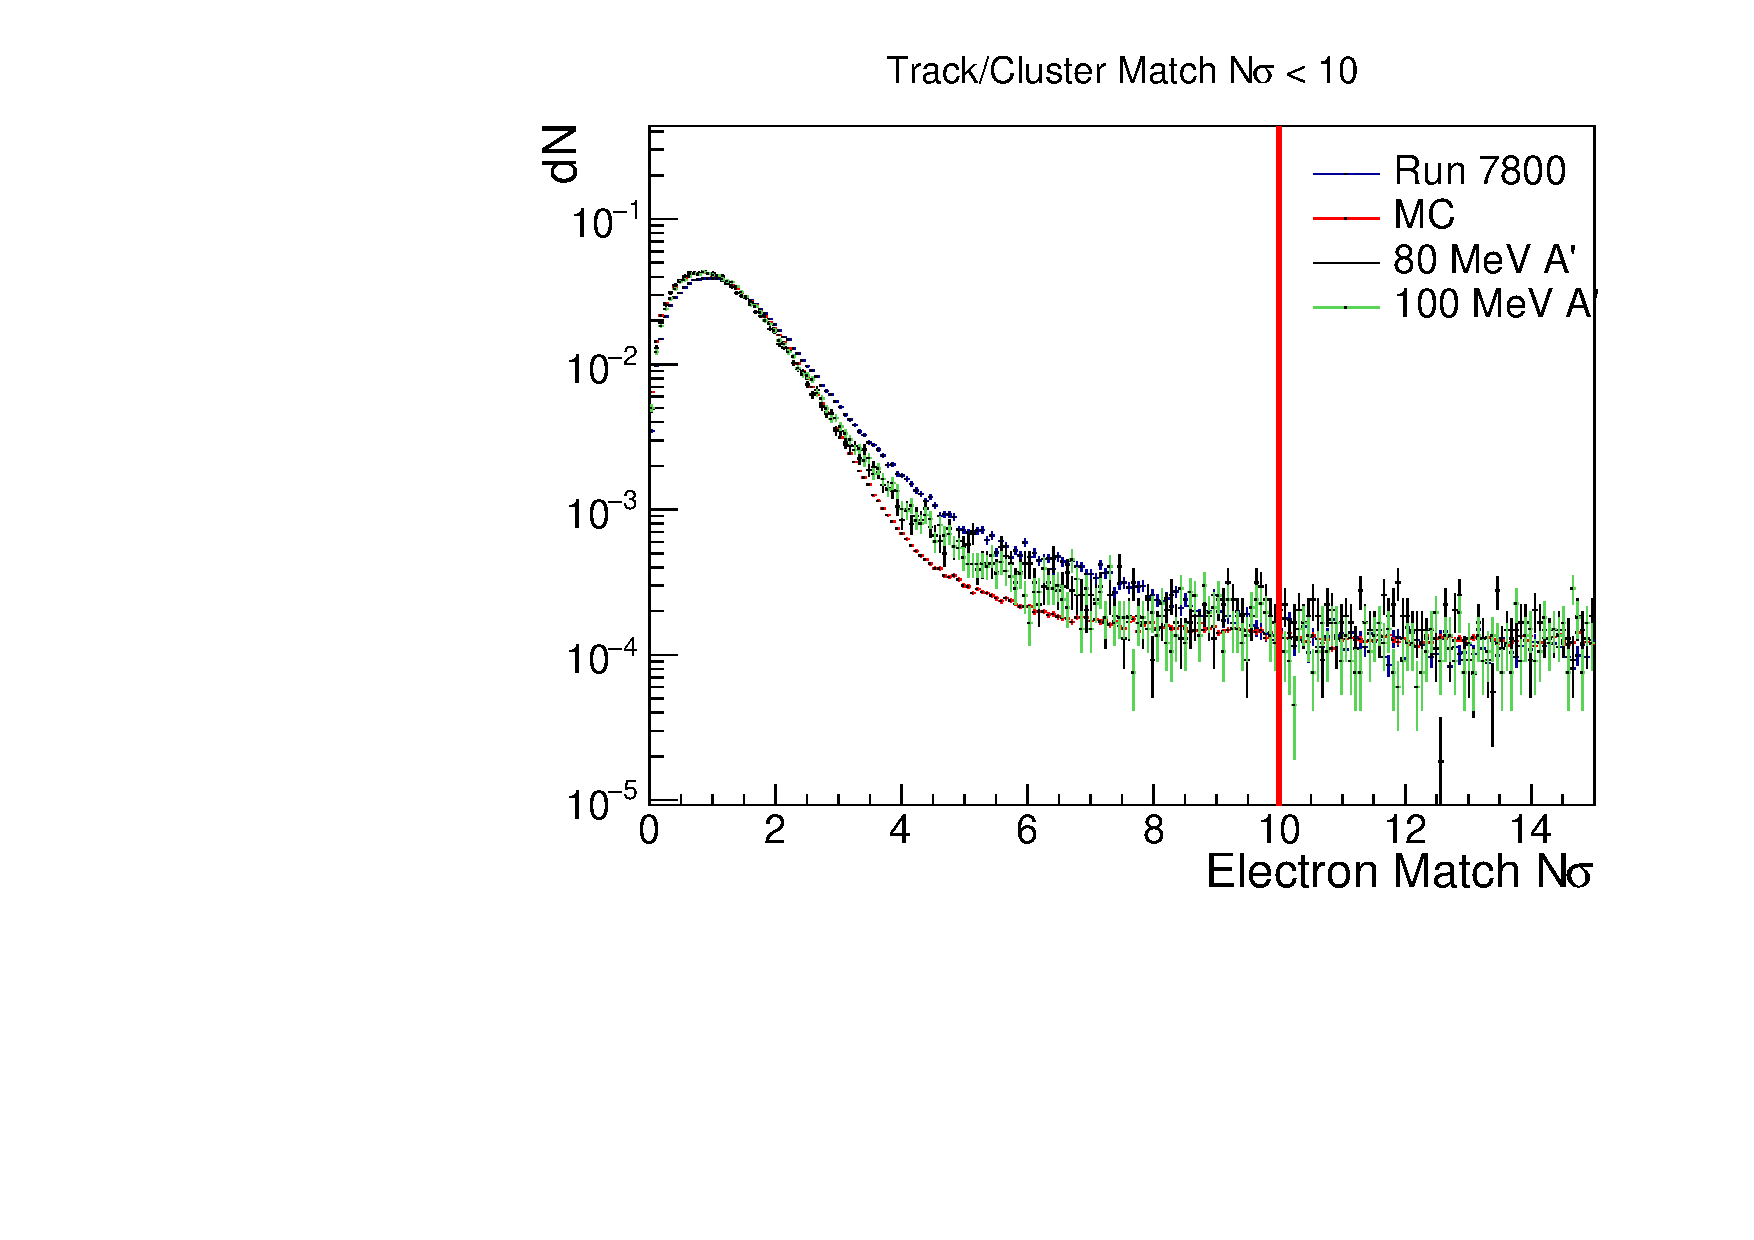
\includegraphics[width=.45\textwidth]{figs/recon/pre_eleMatchChisq.pdf}
    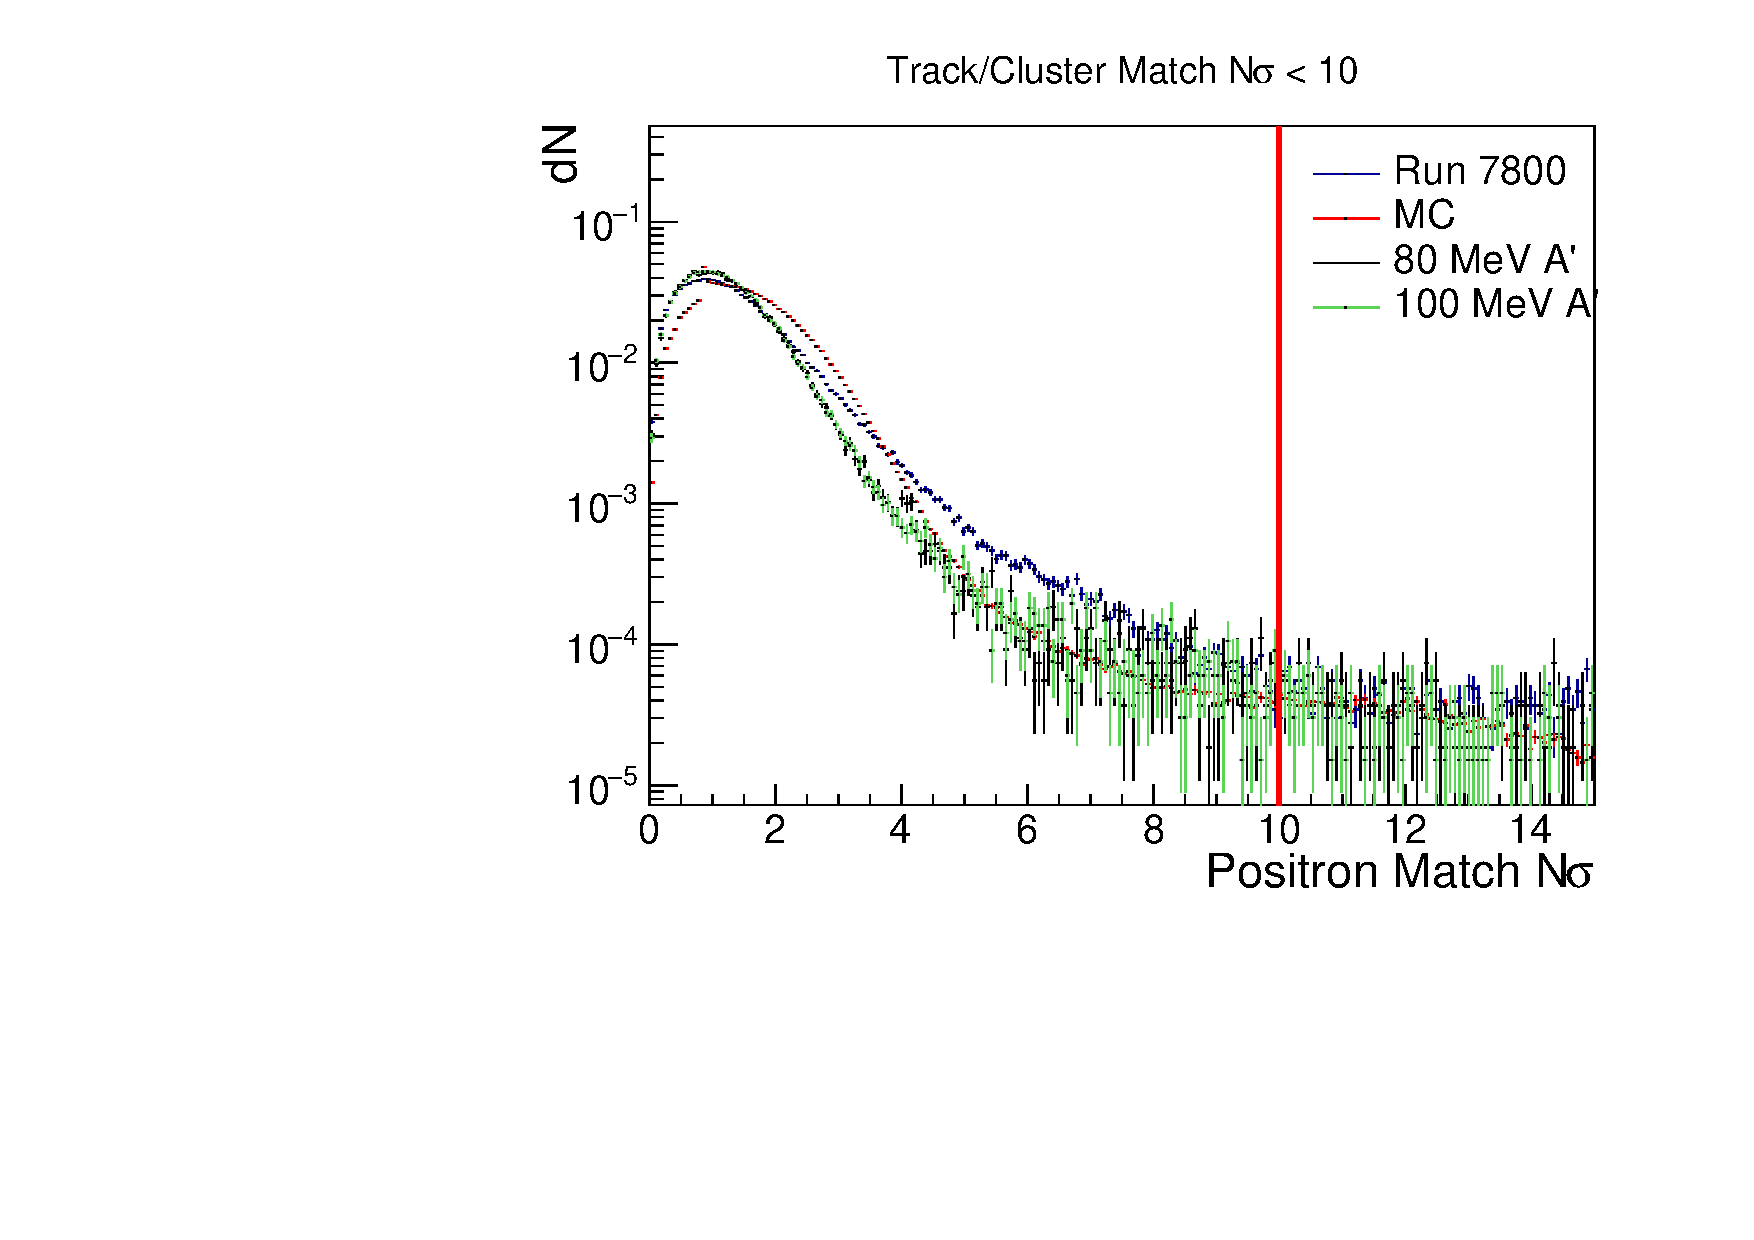
\includegraphics[width=.45\textwidth]{figs/recon/pre_posMatchChisq.pdf}
    \caption{Track-cluster match number of $\sigma$ for electrons (left) and positrons (right). A loose cut is placed at $N_{\sigma}<10$ for both electrons and positrons to eliminate poor track-cluster matches.}
    \label{fig:pre_matchChisq}
\end{figure}

\begin{figure}[t]
    \centering
    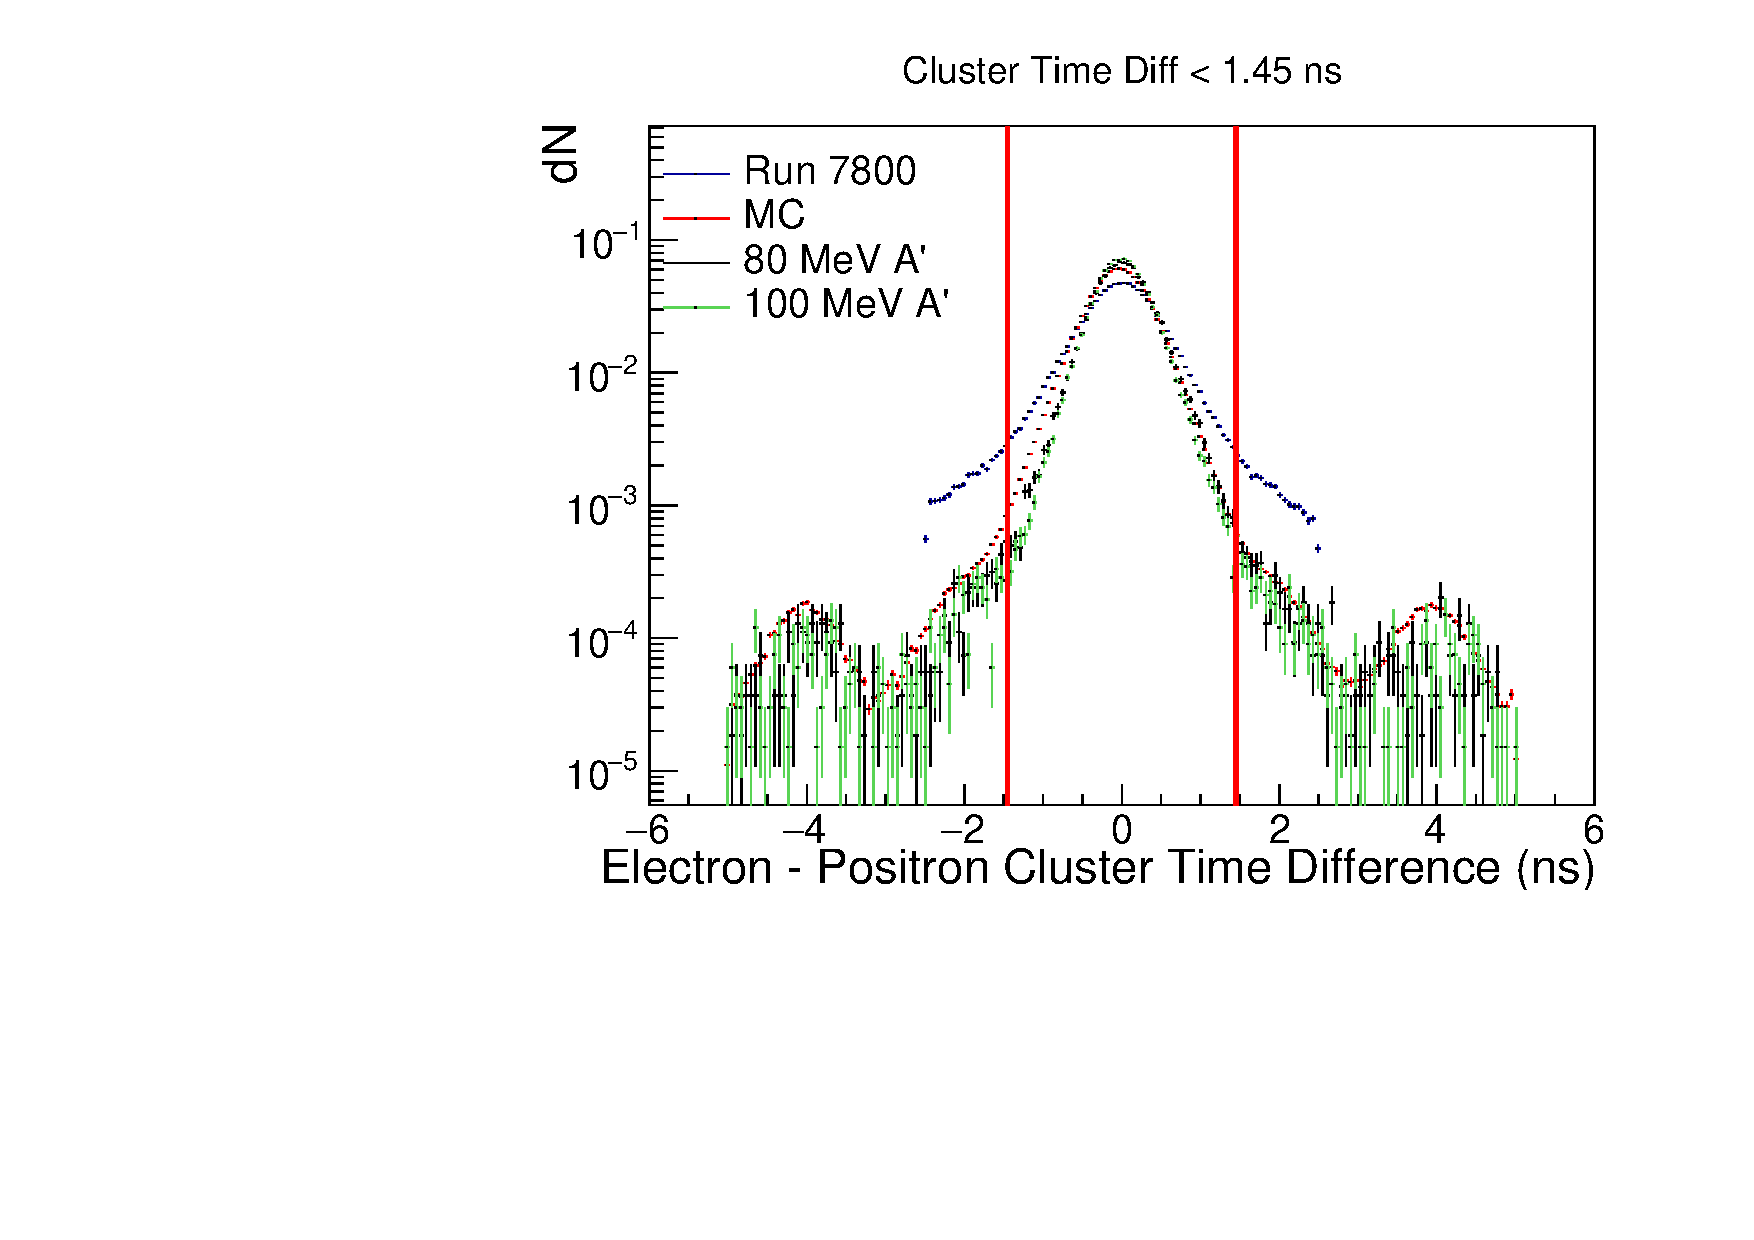
\includegraphics[width=.45\textwidth]{figs/recon/pre_clT.pdf}
    %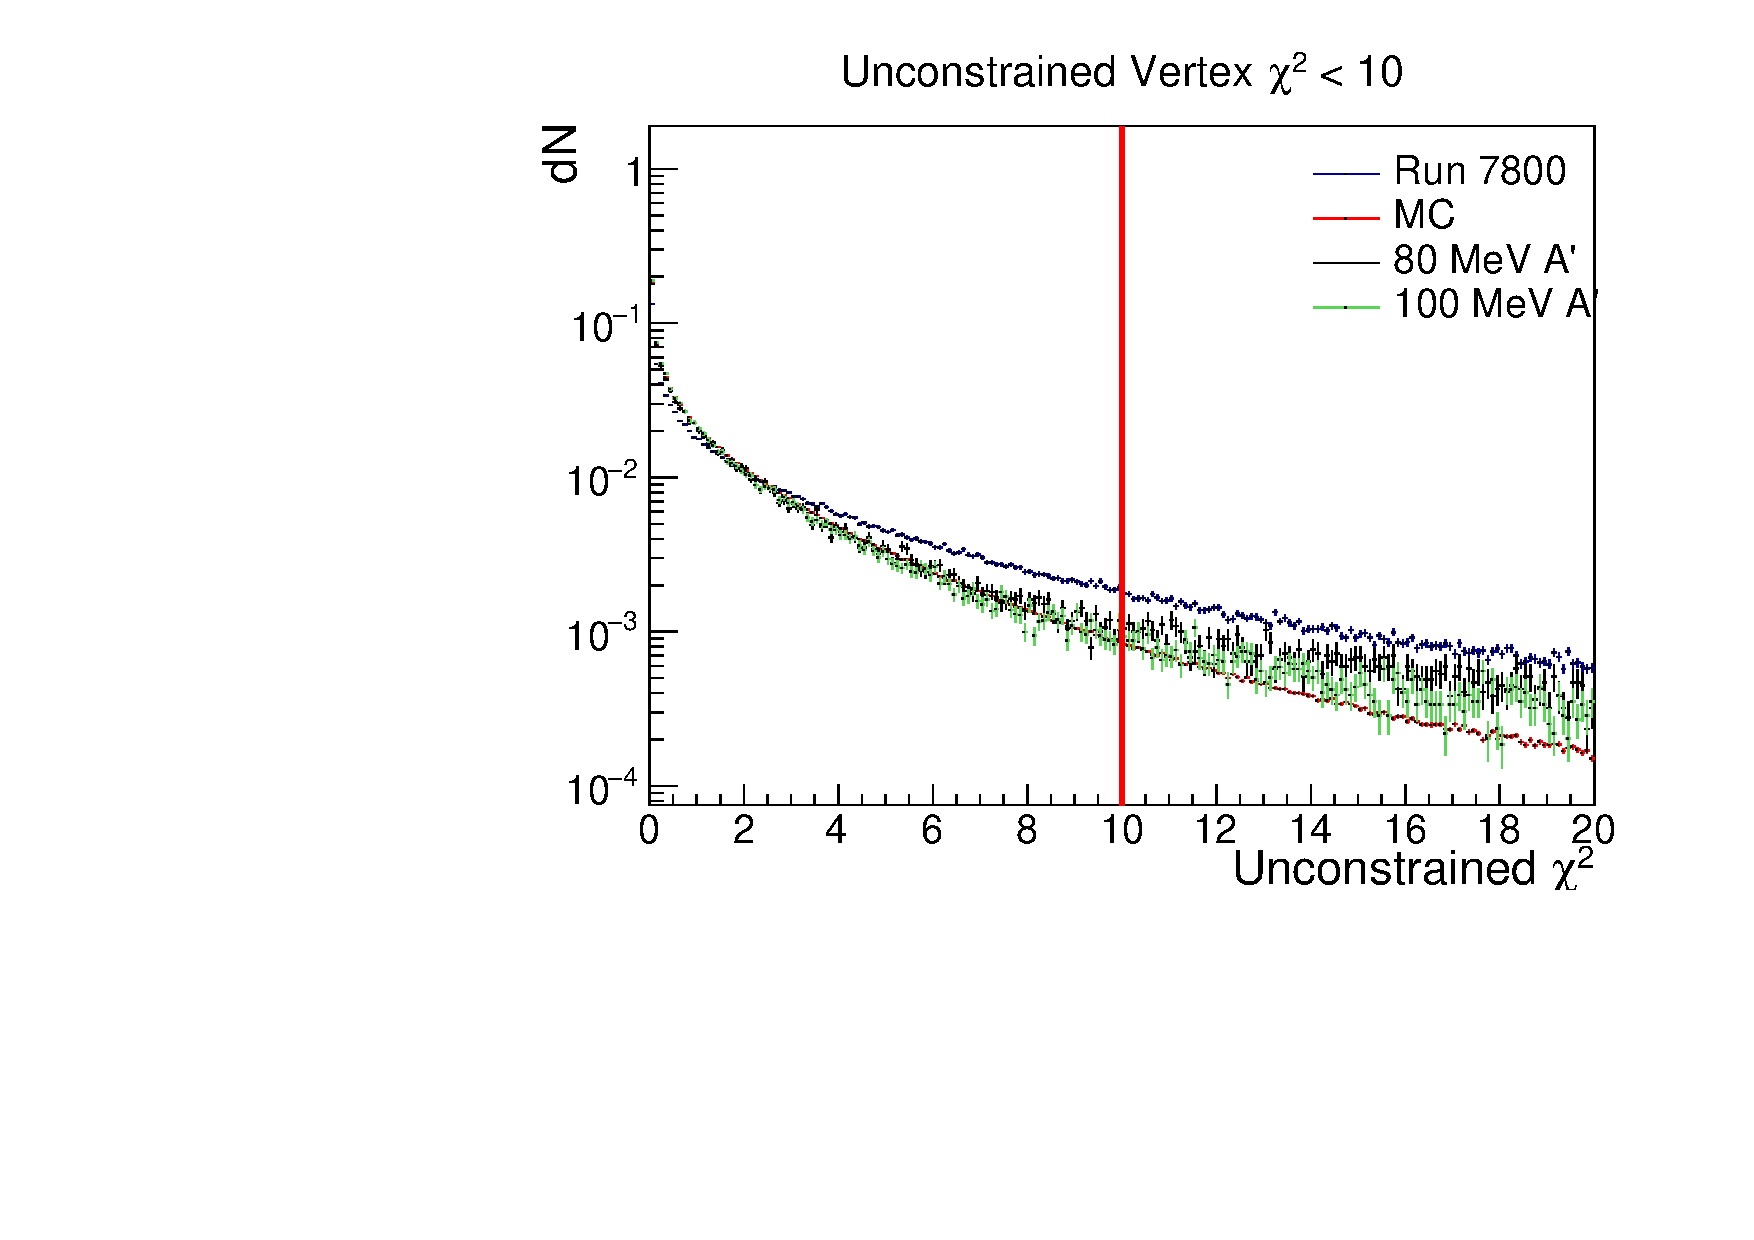
\includegraphics[width=.45\textwidth]{figs/recon/pre_uncChisq.pdf}
    \caption{A cluster time difference cut between electrons and positrons is placed at 1.45 ns to minimize accidentals from other beam bunches (Hall B bunches are spaced at 2 ns). %Right: A loose cut on the unconstrained vertex fit $\chi_{unc}$ is placed at 10 to eliminate poorly reconstructed V0s that can incorrectly reconstruct downstream of the target. There is some mismodeling for the cluster time resolution, and there is some mismodeling in the vertex quality.
    }
    \label{fig:pre_clT_uncChisq}
\end{figure}

In addition, the difference between the track time and the cluster time is required to be less than 4 ns. Before applying this cut, the track time distribution is shifted to zero by correcting the offset, which is approximately 56 ns in data and 43 ns in MC simulation\footnote{There is a discrepancy in the offset between data and MC which can be attributed to the different conditions used. The is also a difference between the offsets in data for preprocessing cuts in Table \ref{tab:mouse_data} (55 ns) and Preselection cuts in Table \ref{tab:preselection} (56 ns). The correct offset is 56 ns; however, the window of 10 ns used for the preprocessing cuts is significantly wider than the 4 ns in the Preselection.}. The cut is loose enough that it is possible to use the same offset correction for each run in data without introducing run-by-run systematic effects, but it also further reduces $e^{+}e^{-}$ pairs where one of the tracks is mismatched to the corresponding cluster. This is the same cut value for cluster-track time difference that was used in previous displaced vertexing and resonance search and is shown in Fig. \ref{fig:pre_trkT} \cite{adrian2018search} \cite{article}.

\begin{figure}[t]
    \centering
    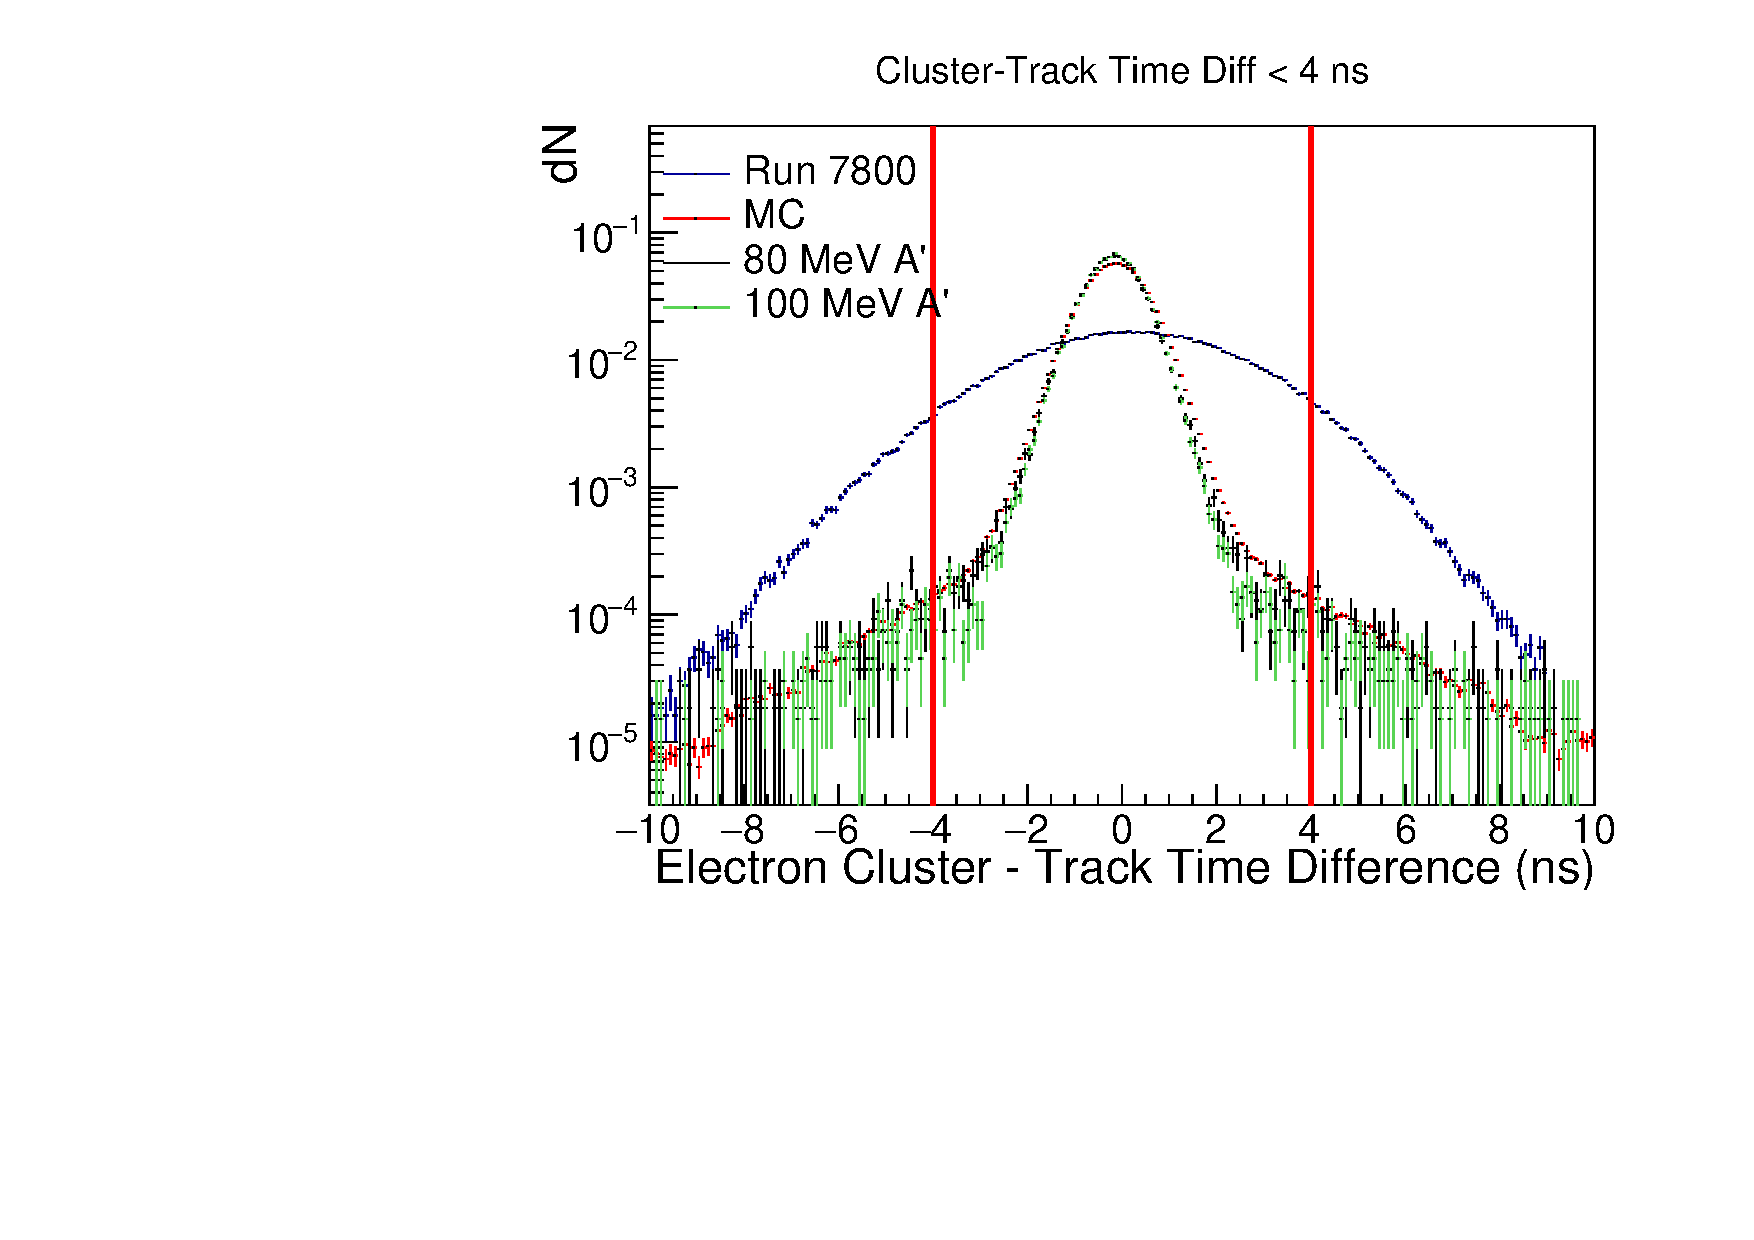
\includegraphics[width=.45\textwidth]{figs/recon/pre_eleTrkT.pdf}
    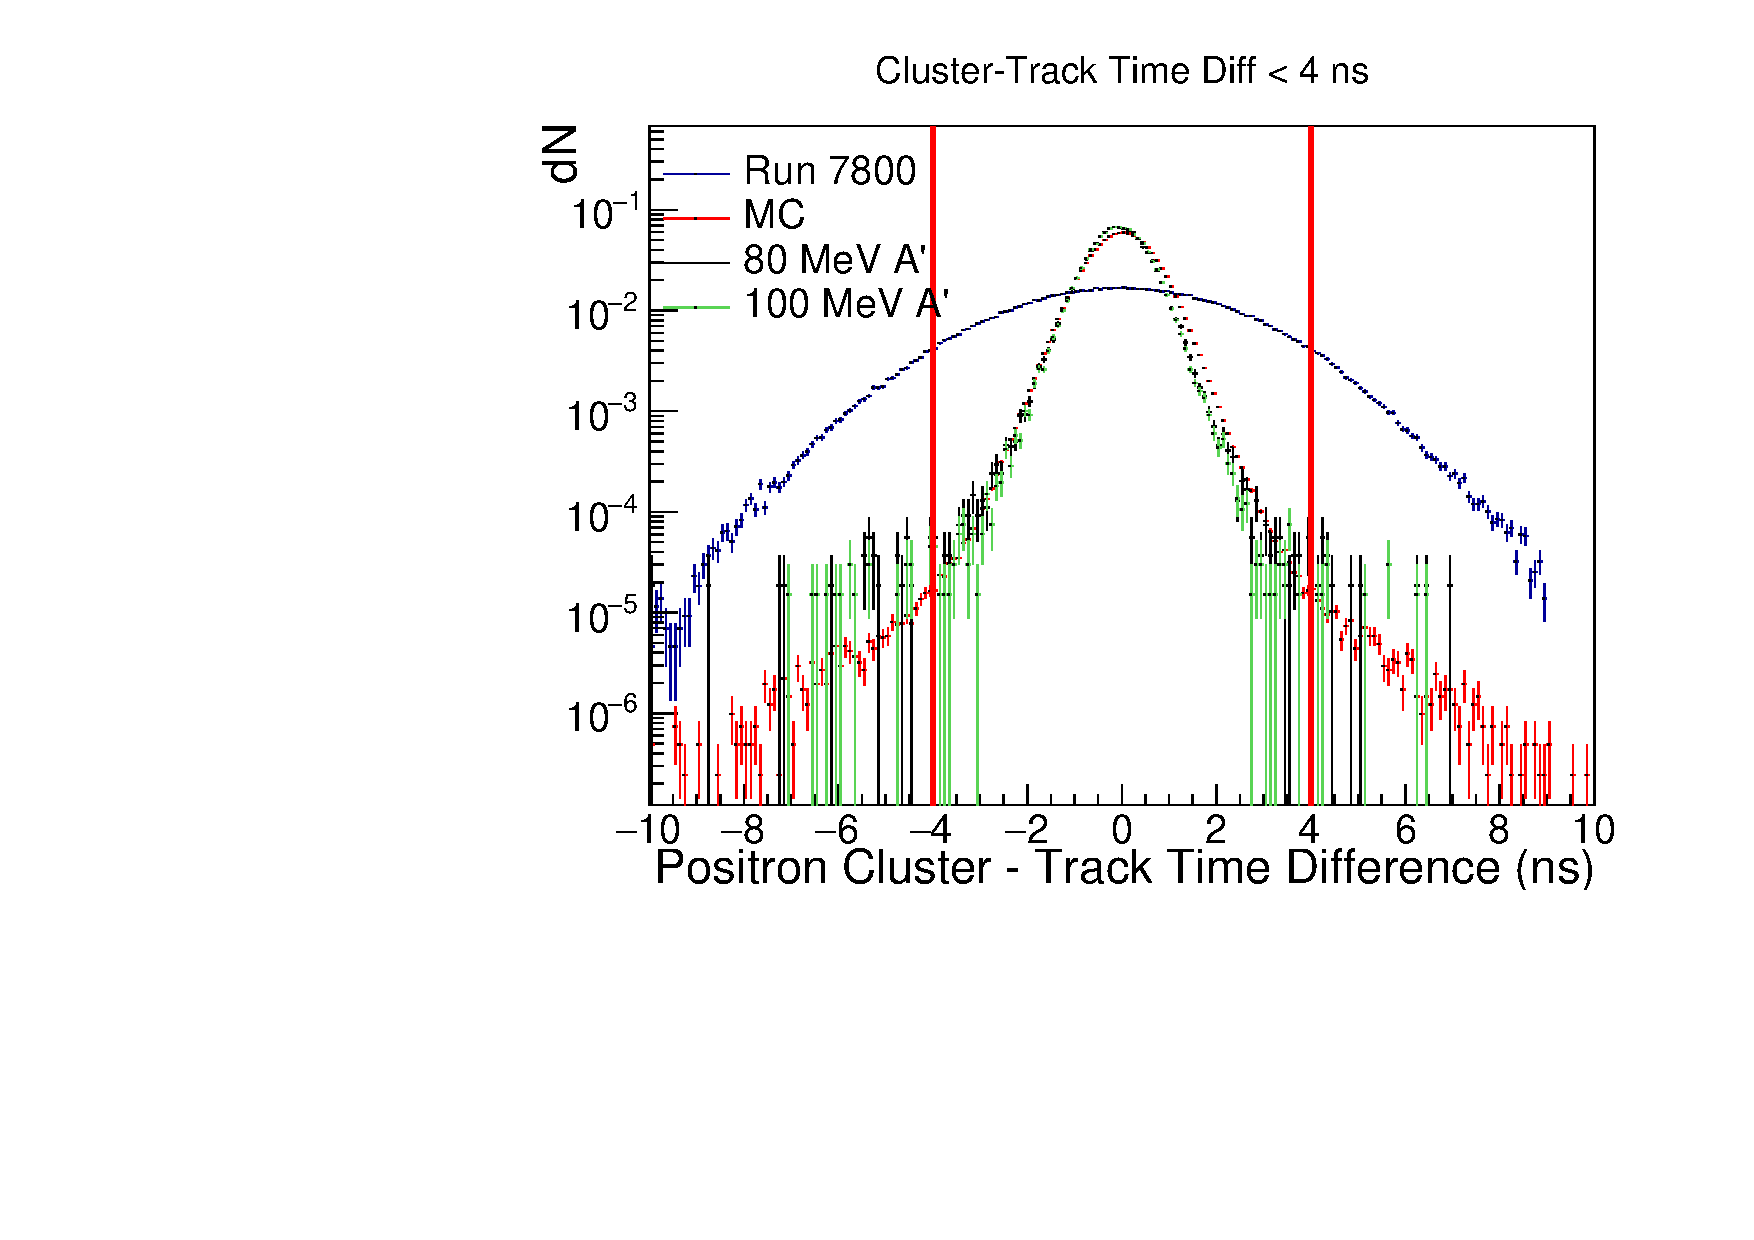
\includegraphics[width=.45\textwidth]{figs/recon/pre_posTrkT.pdf}
    \caption{Cluster-track time difference (with the time offset from Table \ref{tab:preselection}) for electrons (left) and positrons (right). A cut is placed at a time difference of 4 ns for both electrons and positrons to eliminate out of time tracks. There is significant mis-modeling for the track time resolution; however, this is a data-driven cut.}
    \label{fig:pre_trkT}
\end{figure}

Electrons are required to have a momentum magnitude less than 1.75 GeV in order to remove the contribution from full energy electrons - that is electrons that scatter elastically off the nucleus of the tungsten target. In addition, loose cuts on the minimum particle momentum at 0.4 GeV (since low momentum daughter particles are not expected from $\aprime$s) and maximum $V_0$ momentum 2.4 GeV (above which no signal is expected) are also shared with the resonance search. The electron momentum cuts are shown in Fig. \ref{fig:pre_eleP_posP} and the positron momentum cut and the maximum V0 momentum cut are shown in Fig. \ref{fig:pre_V0p}.

\begin{figure}[t]
    \centering
    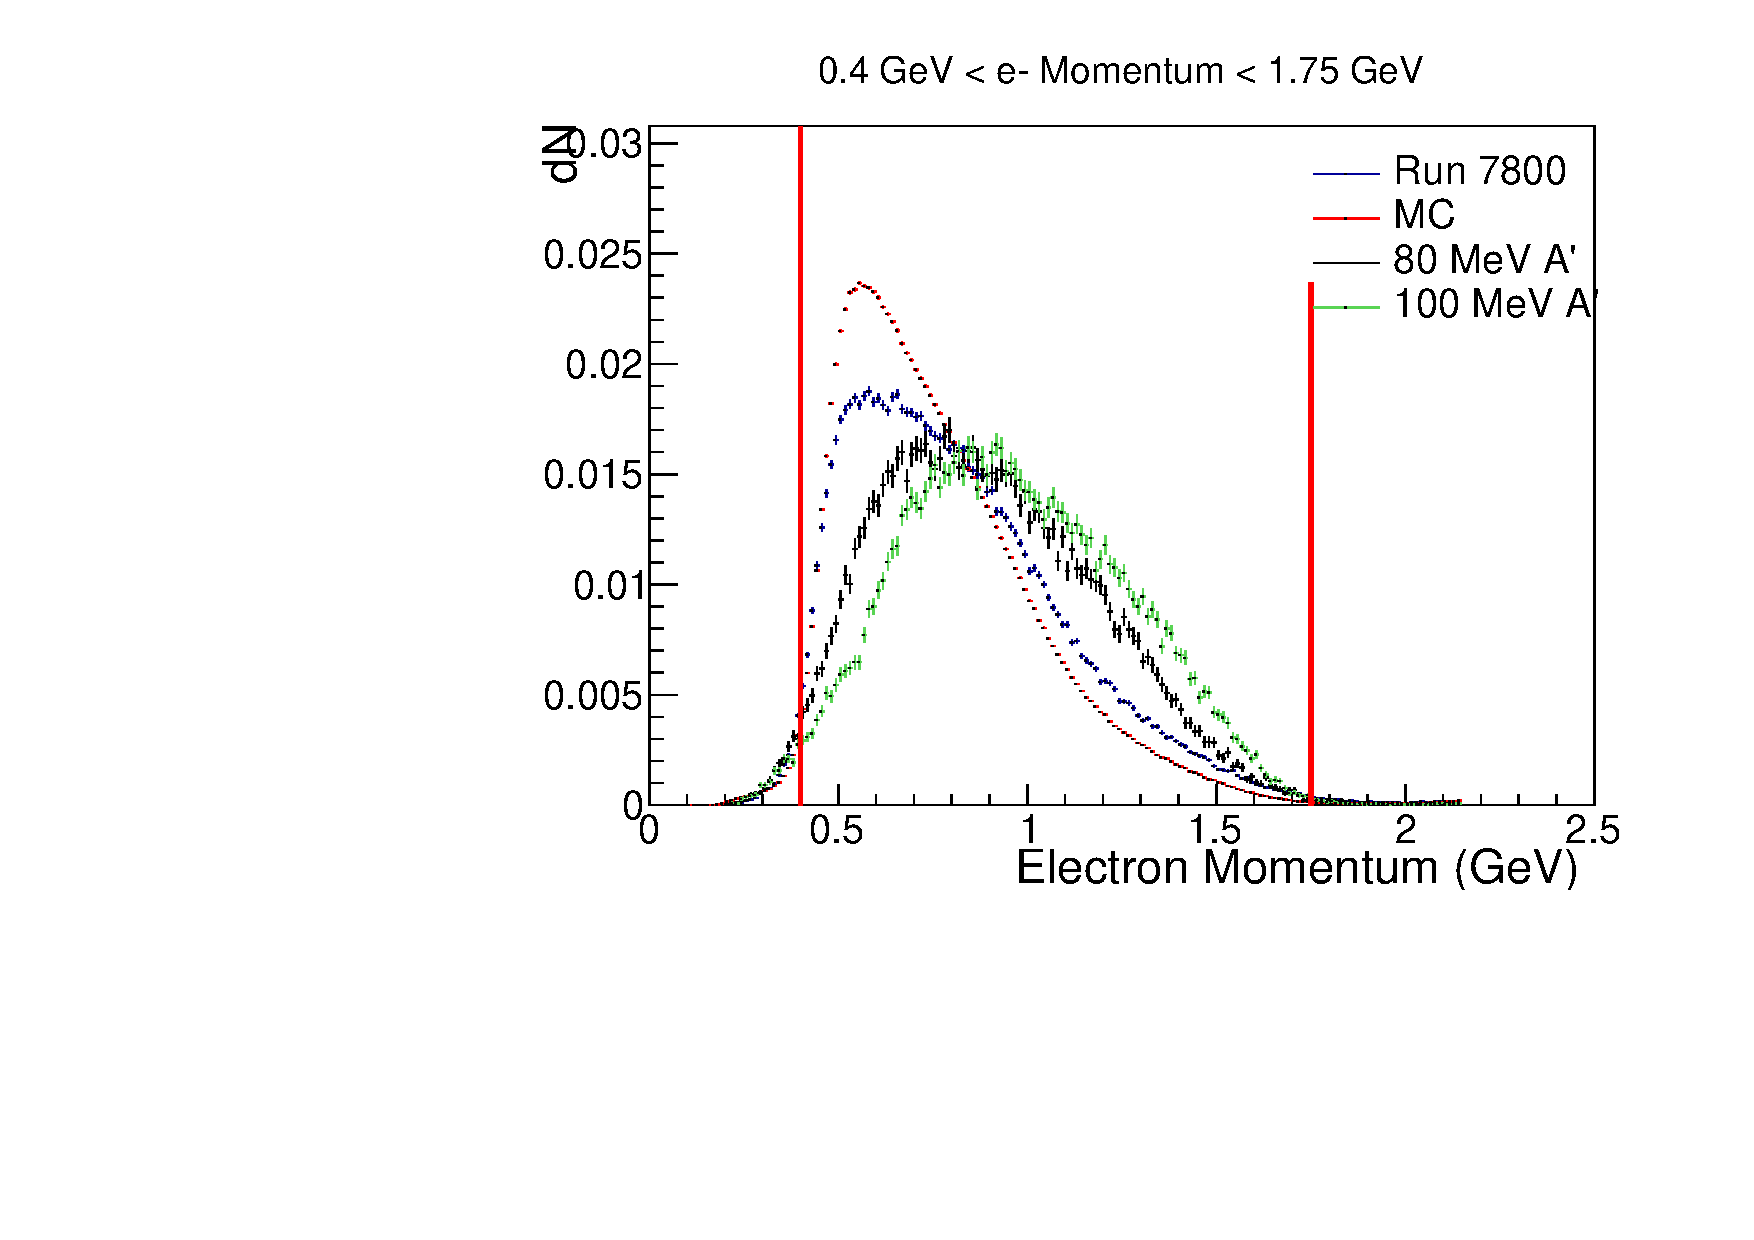
\includegraphics[width=.45\textwidth]{figs/recon/pre_eleP.pdf}
    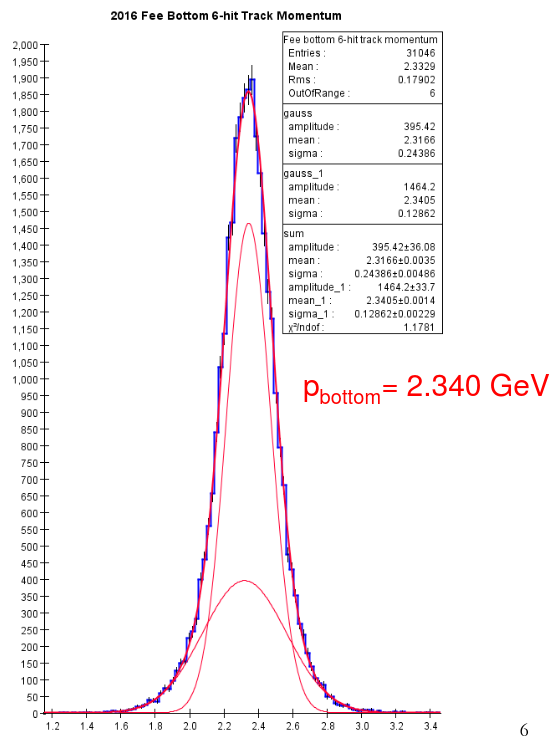
\includegraphics[width=.35\textwidth]{figs/recon/feep.png}
    \caption{Electron momentum has a minimum momentum cut at 0.4 GeV in order to reduce low momentum particles that have larger multiple scattering. A maximum momentum cut is placed at 1.75 GeV to eliminate V0s that reconstruct with elastically-scattered electrons in the target. Left: The plot of electron momentum after preprocessing. Right: A plot of the electron momentum used to study full-energy electrons (since most elastically-scatter electrons are cut away during preprocessing). There is some mis-modeling for individual particle momenta particularly at low momentum.}
    \label{fig:pre_eleP_posP}
\end{figure}

\begin{figure}[t]
    \centering
    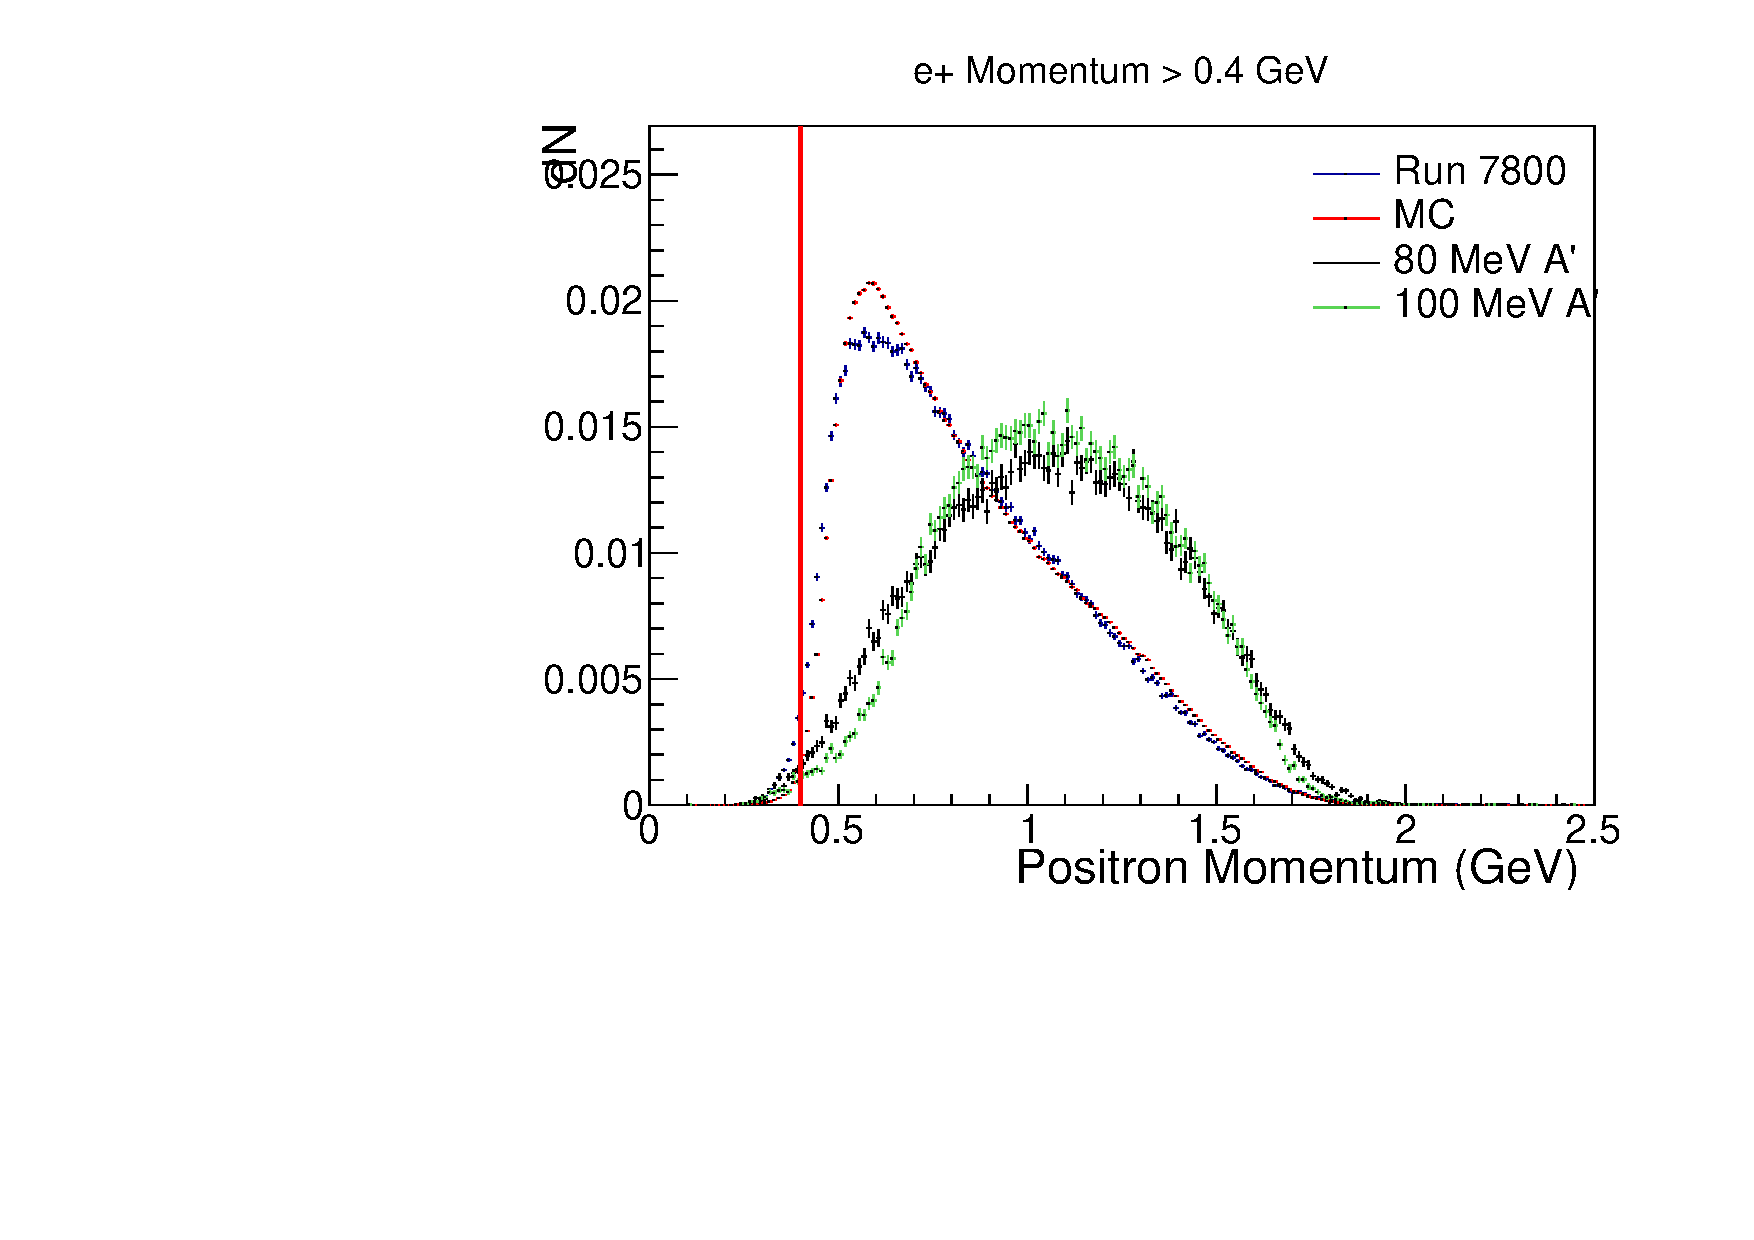
\includegraphics[width=.45\textwidth]{figs/recon/pre_posP.pdf}
    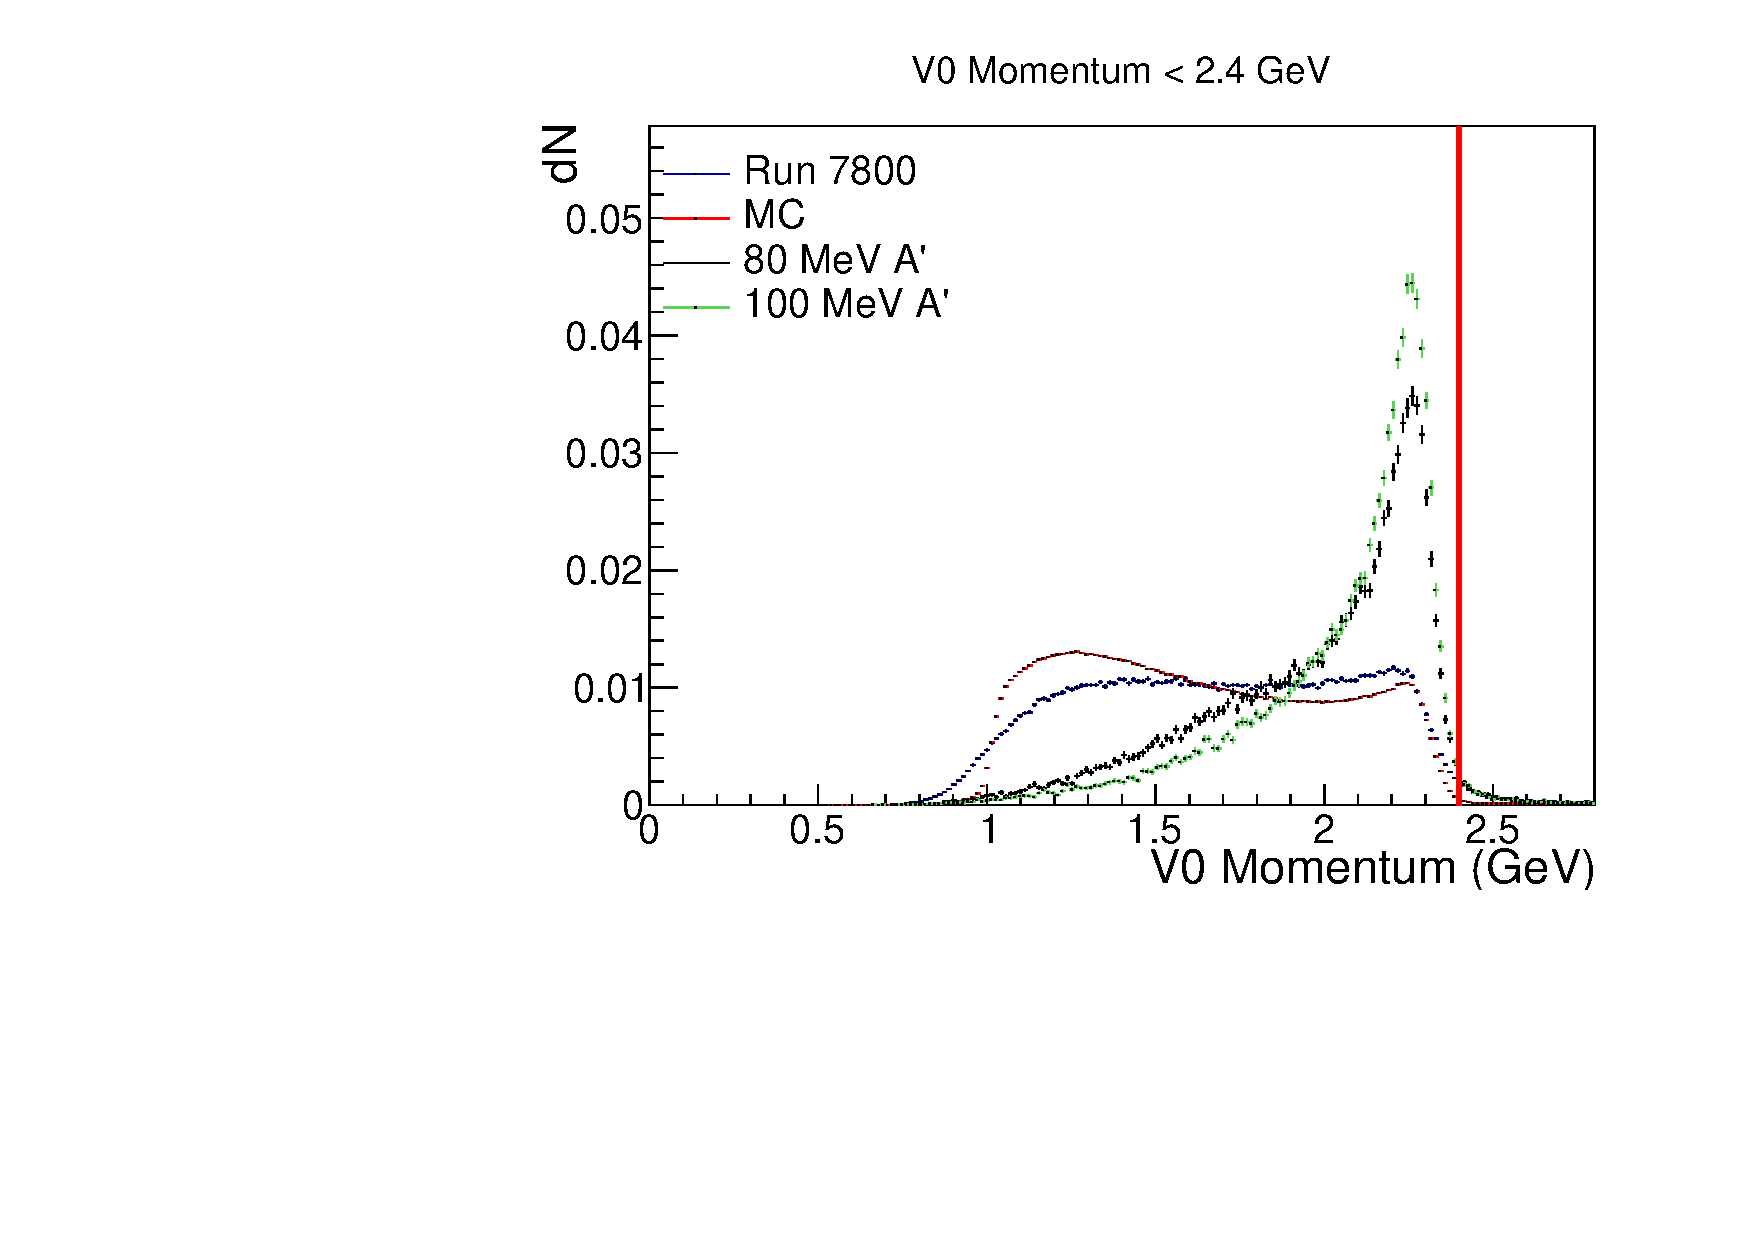
\includegraphics[width=.45\textwidth]{figs/recon/pre_uncP.pdf}
    %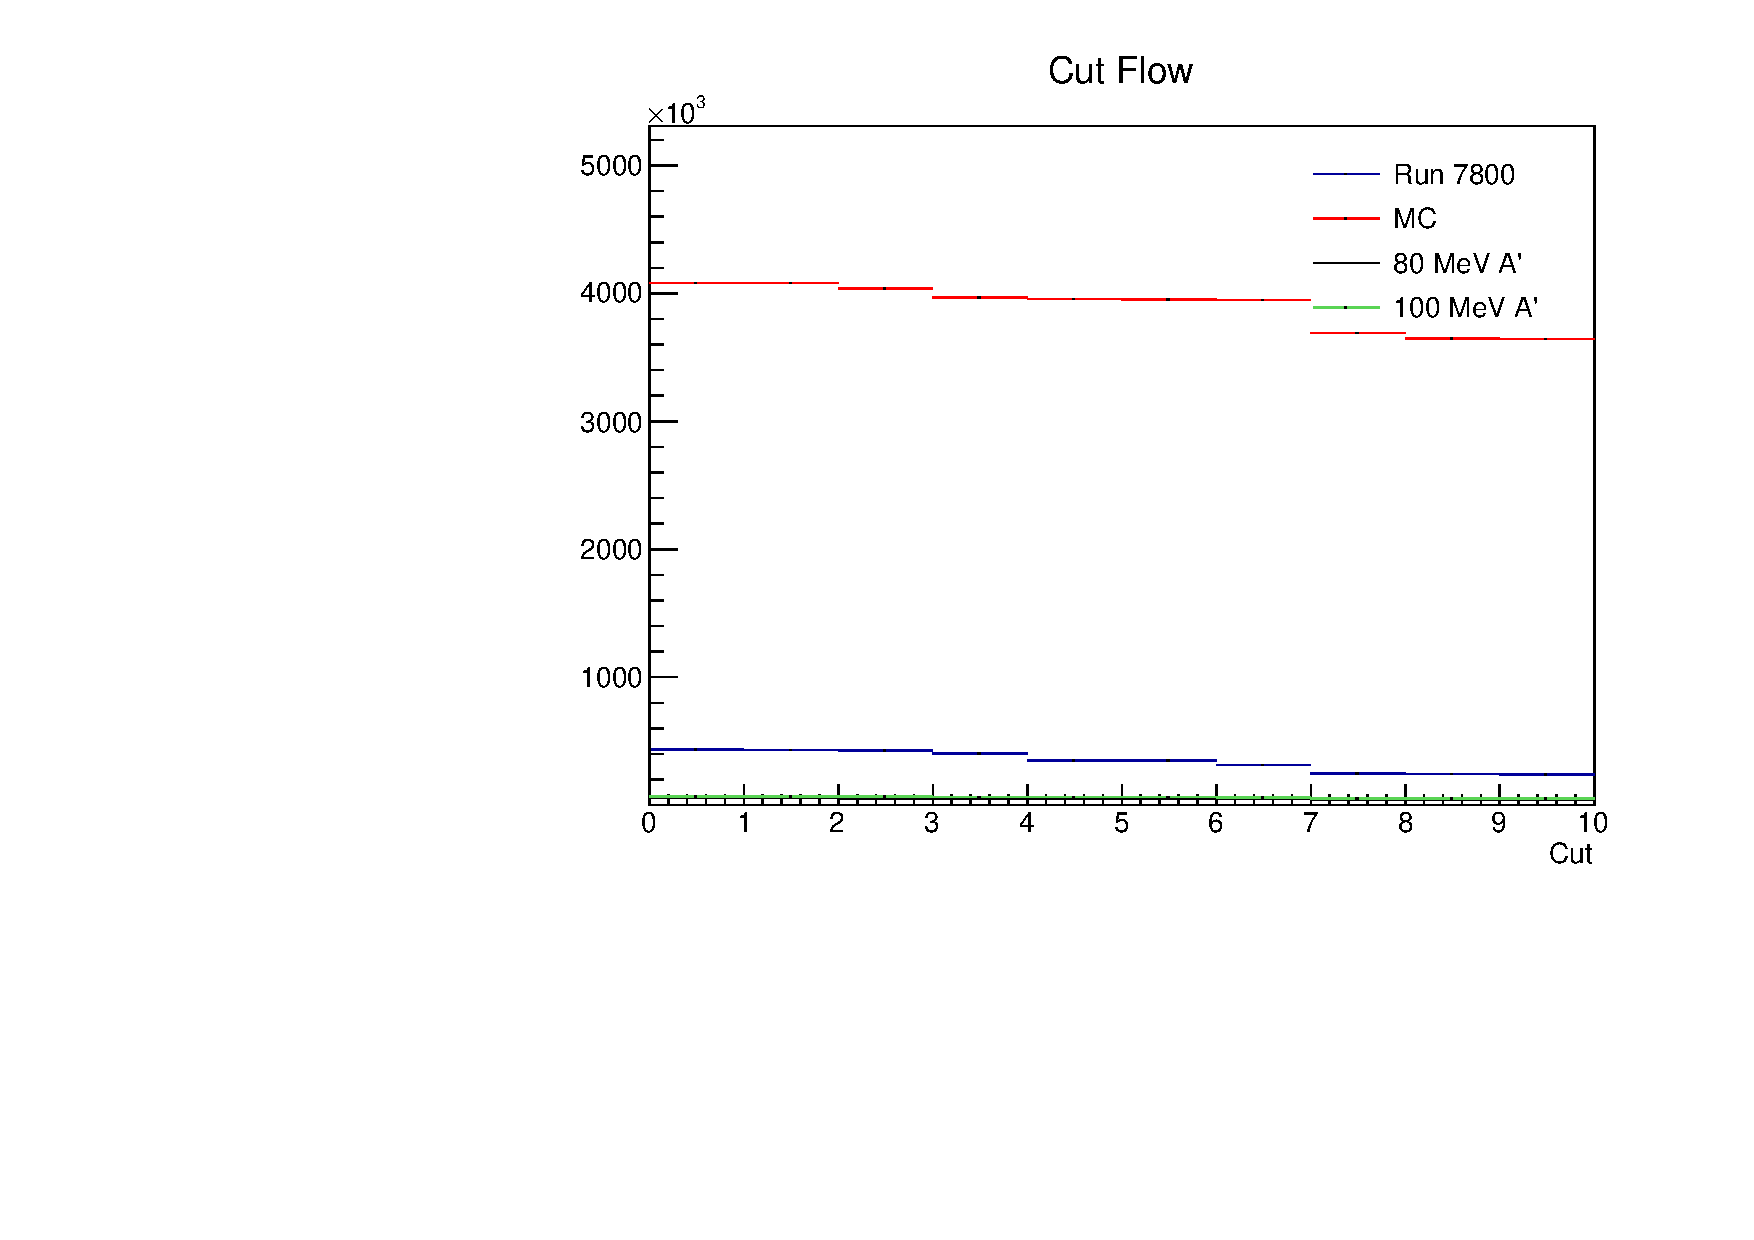
\includegraphics[width=.45\textwidth]{figs/recon/pre_cutflow.pdf}
    \caption{Left: Positron momentum has a minimum momentum cut at 0.4 GeV in order to reduce low momentum particles that have larger multiple scattering. Right: A maximum V0 momentum cut is placed at 2.4 GeV since signal is not expected far above the beam energy at 2.3 GeV.}
    \label{fig:pre_V0p}
\end{figure}

 Poorly fit tracks and vertices can lead to falsely reconstructed vertices downstream of the target. Both tracks are required to have a track quality of $\chi^{2}/dof$ (degrees of freedom) less than 6 which is a relatively loose requirement that was used for the 2015 Displaced Vertex Search \cite{adrian2018search}. Each vertex is required to a vertex fit quality on the unconstrained vertex of at least have a $\chi^{2}_{unc} < 10$ which is a loose requirement. The track and vertex quality are shown in Fig. \ref{fig:pre_trkChisq} and Fig. \ref{fig:pre_clT_uncChisq2}, respectively.
 
 \begin{figure}[t]
    \centering
    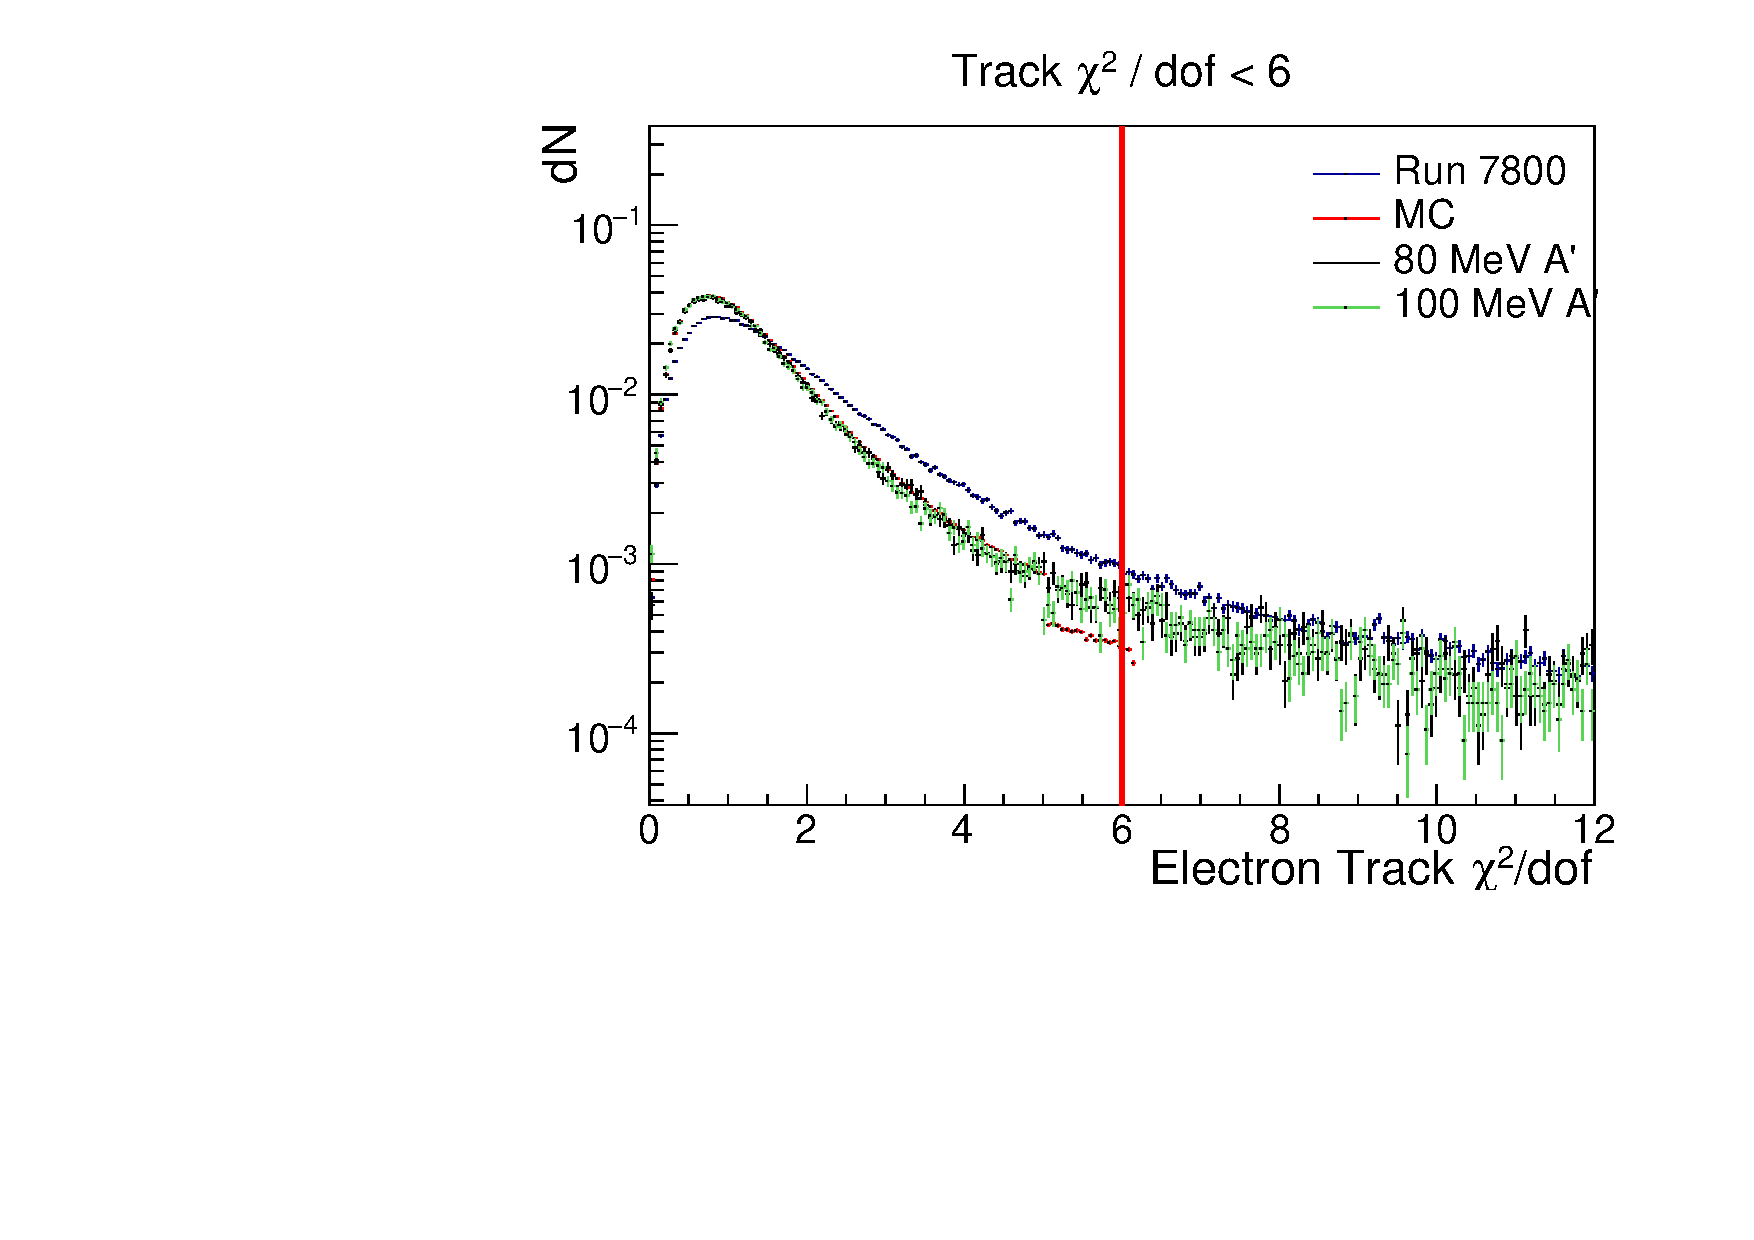
\includegraphics[width=.45\textwidth]{figs/recon/pre_eleTrkChisq.pdf}
    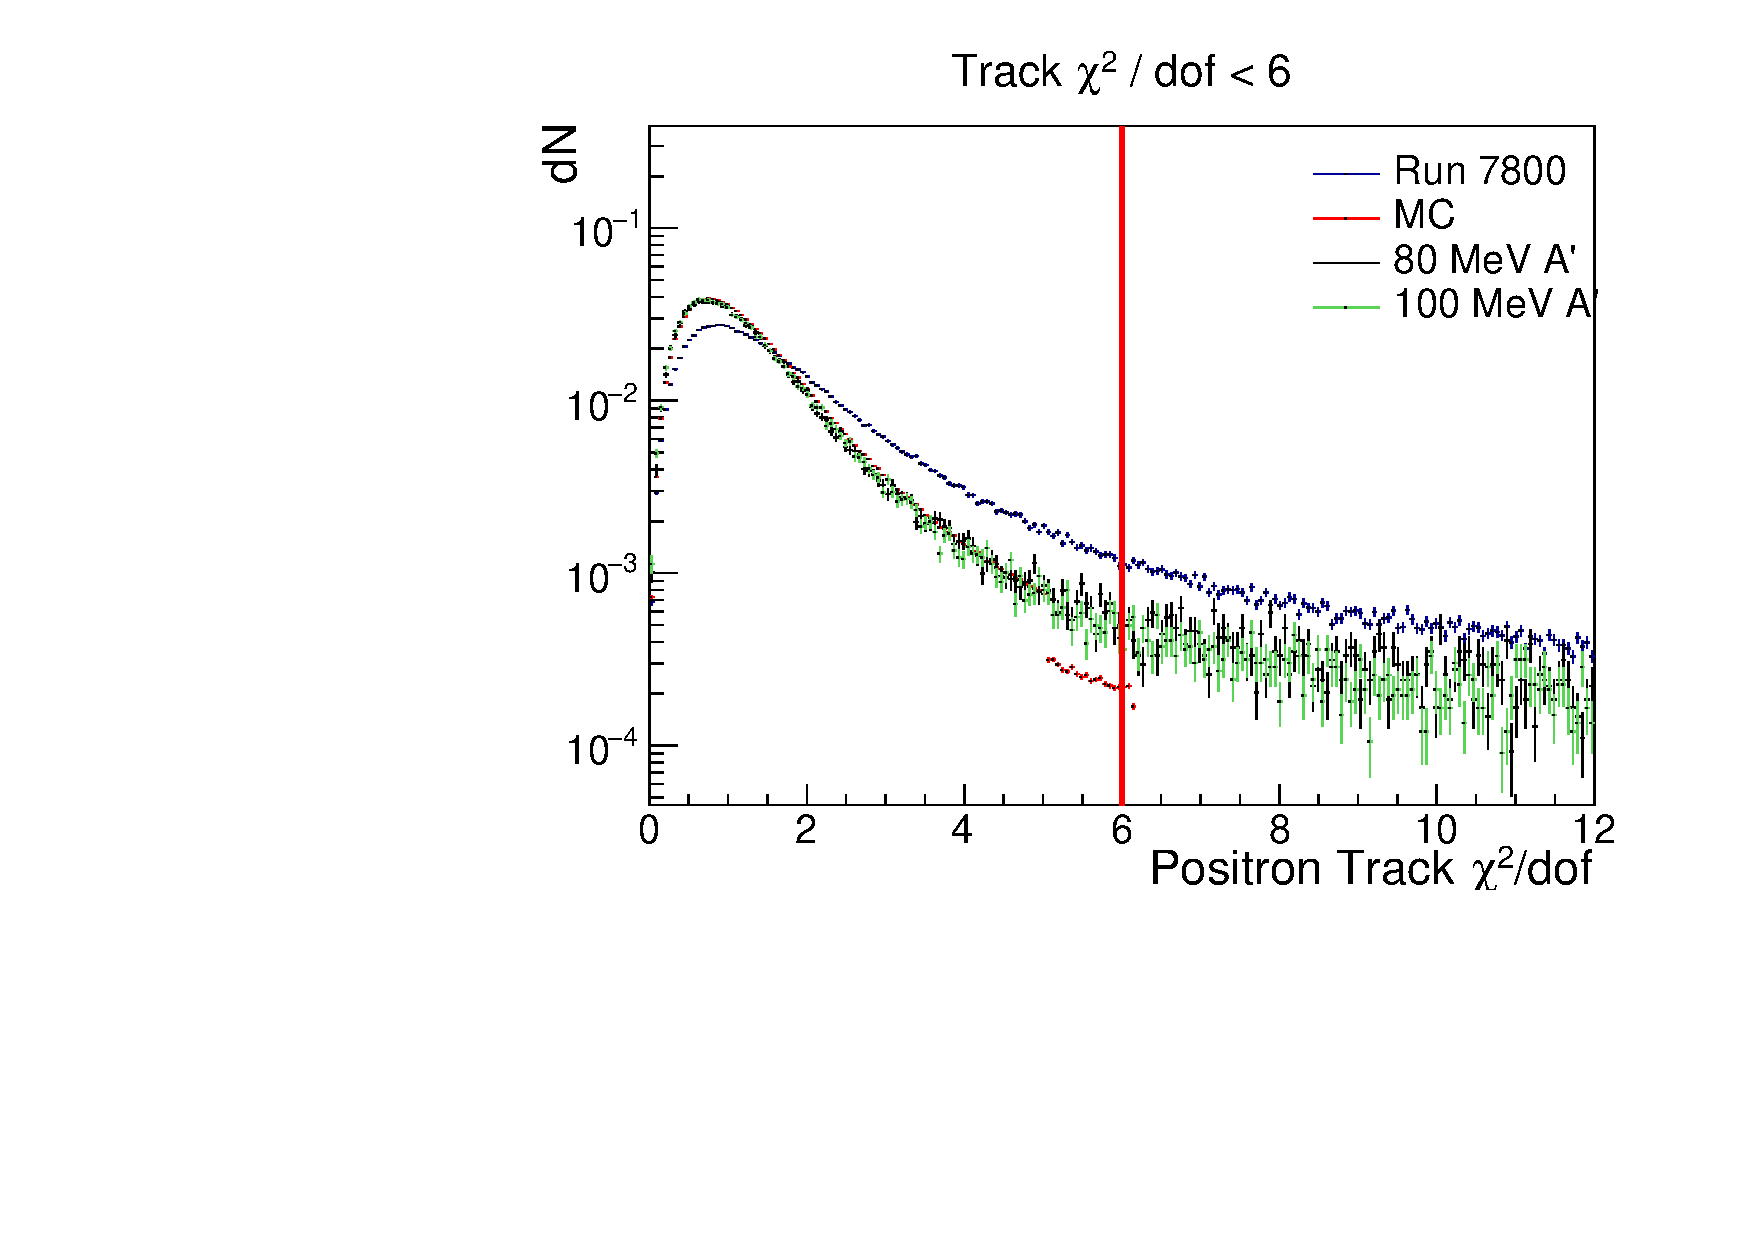
\includegraphics[width=.45\textwidth]{figs/recon/pre_posTrkChisq.pdf}
    \caption{Track $\chi^2$ per degrees of freedom (dof) for electrons (left) and positrons (right). A cut is placed at $\chi^2<6$ for both electrons and positrons to eliminate poor tracks that can falsely reconstruct downstream of the target.}
    \label{fig:pre_trkChisq}
\end{figure}

\begin{figure}[t]
    \centering
    %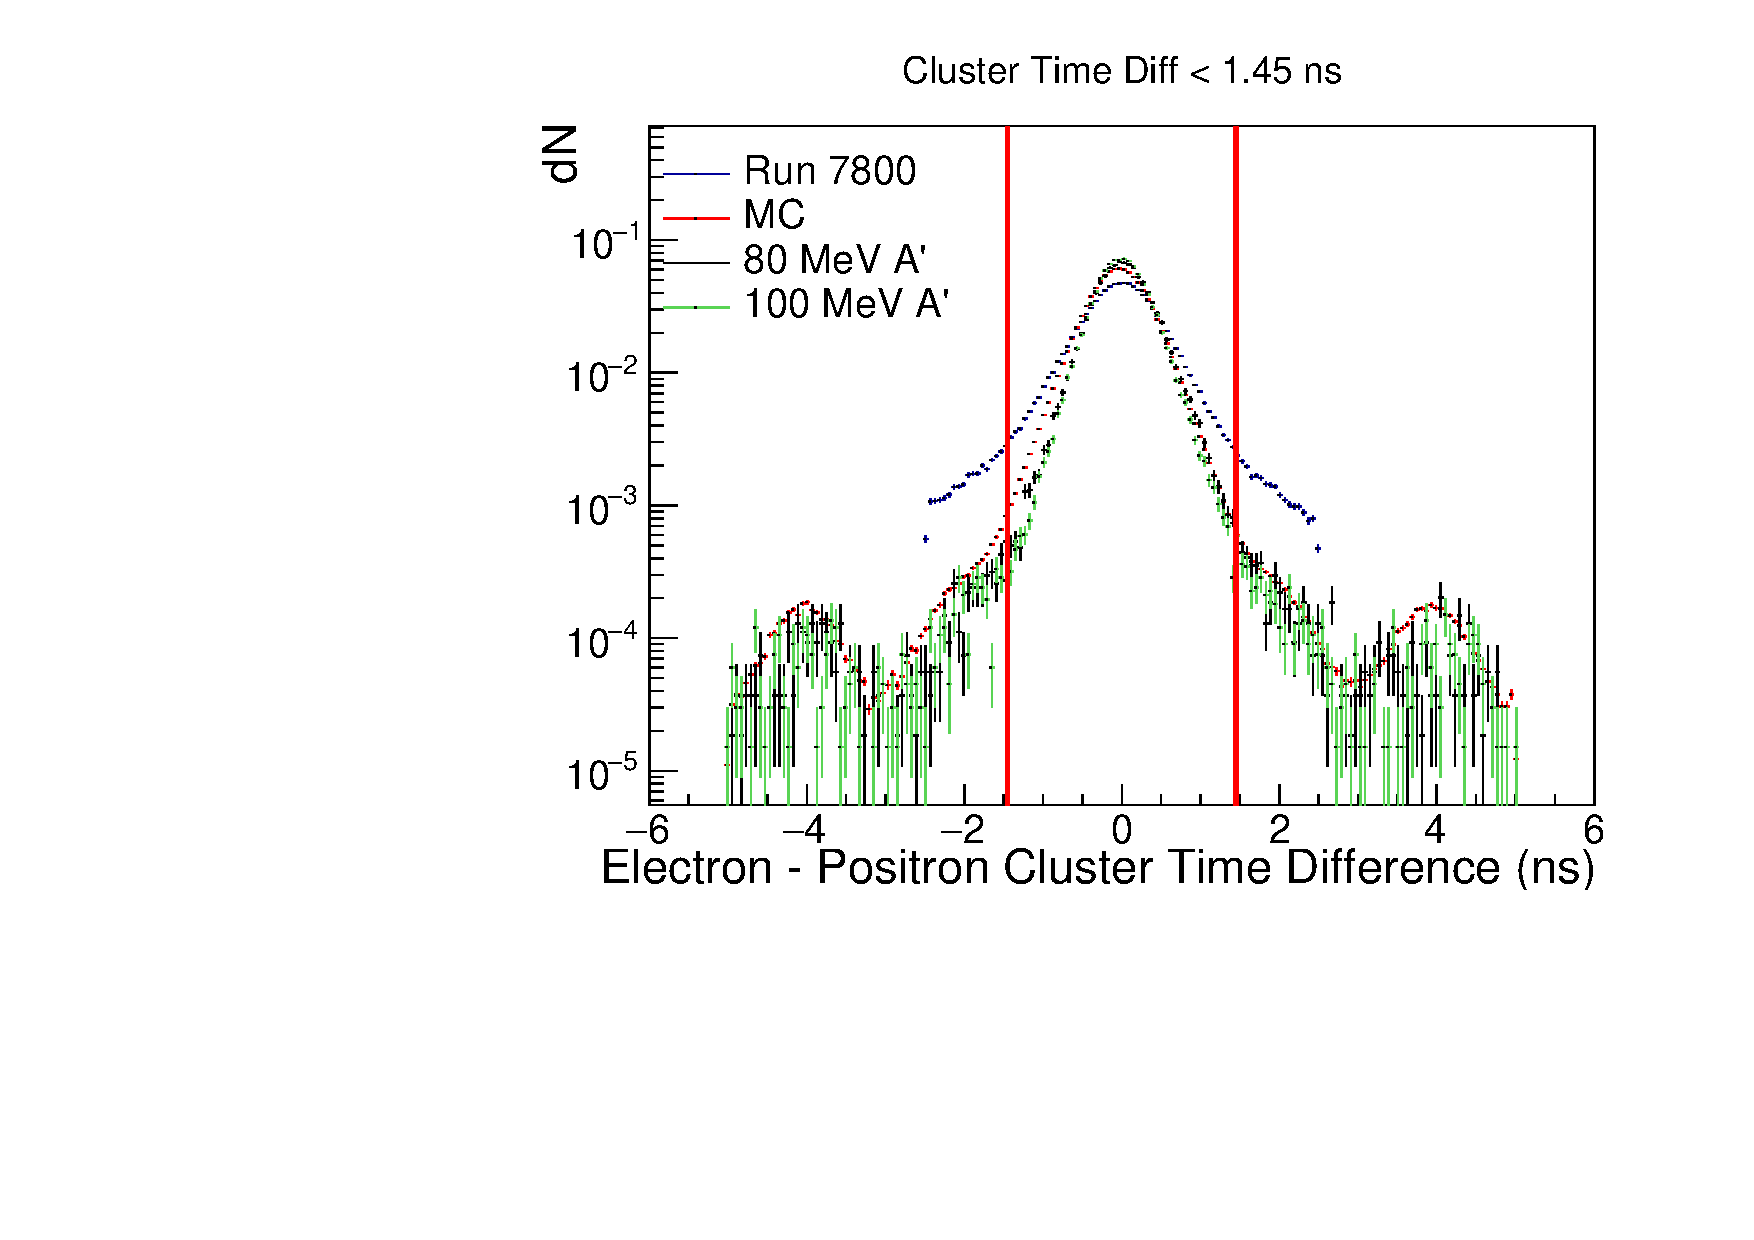
\includegraphics[width=.45\textwidth]{figs/recon/pre_clT.pdf}
    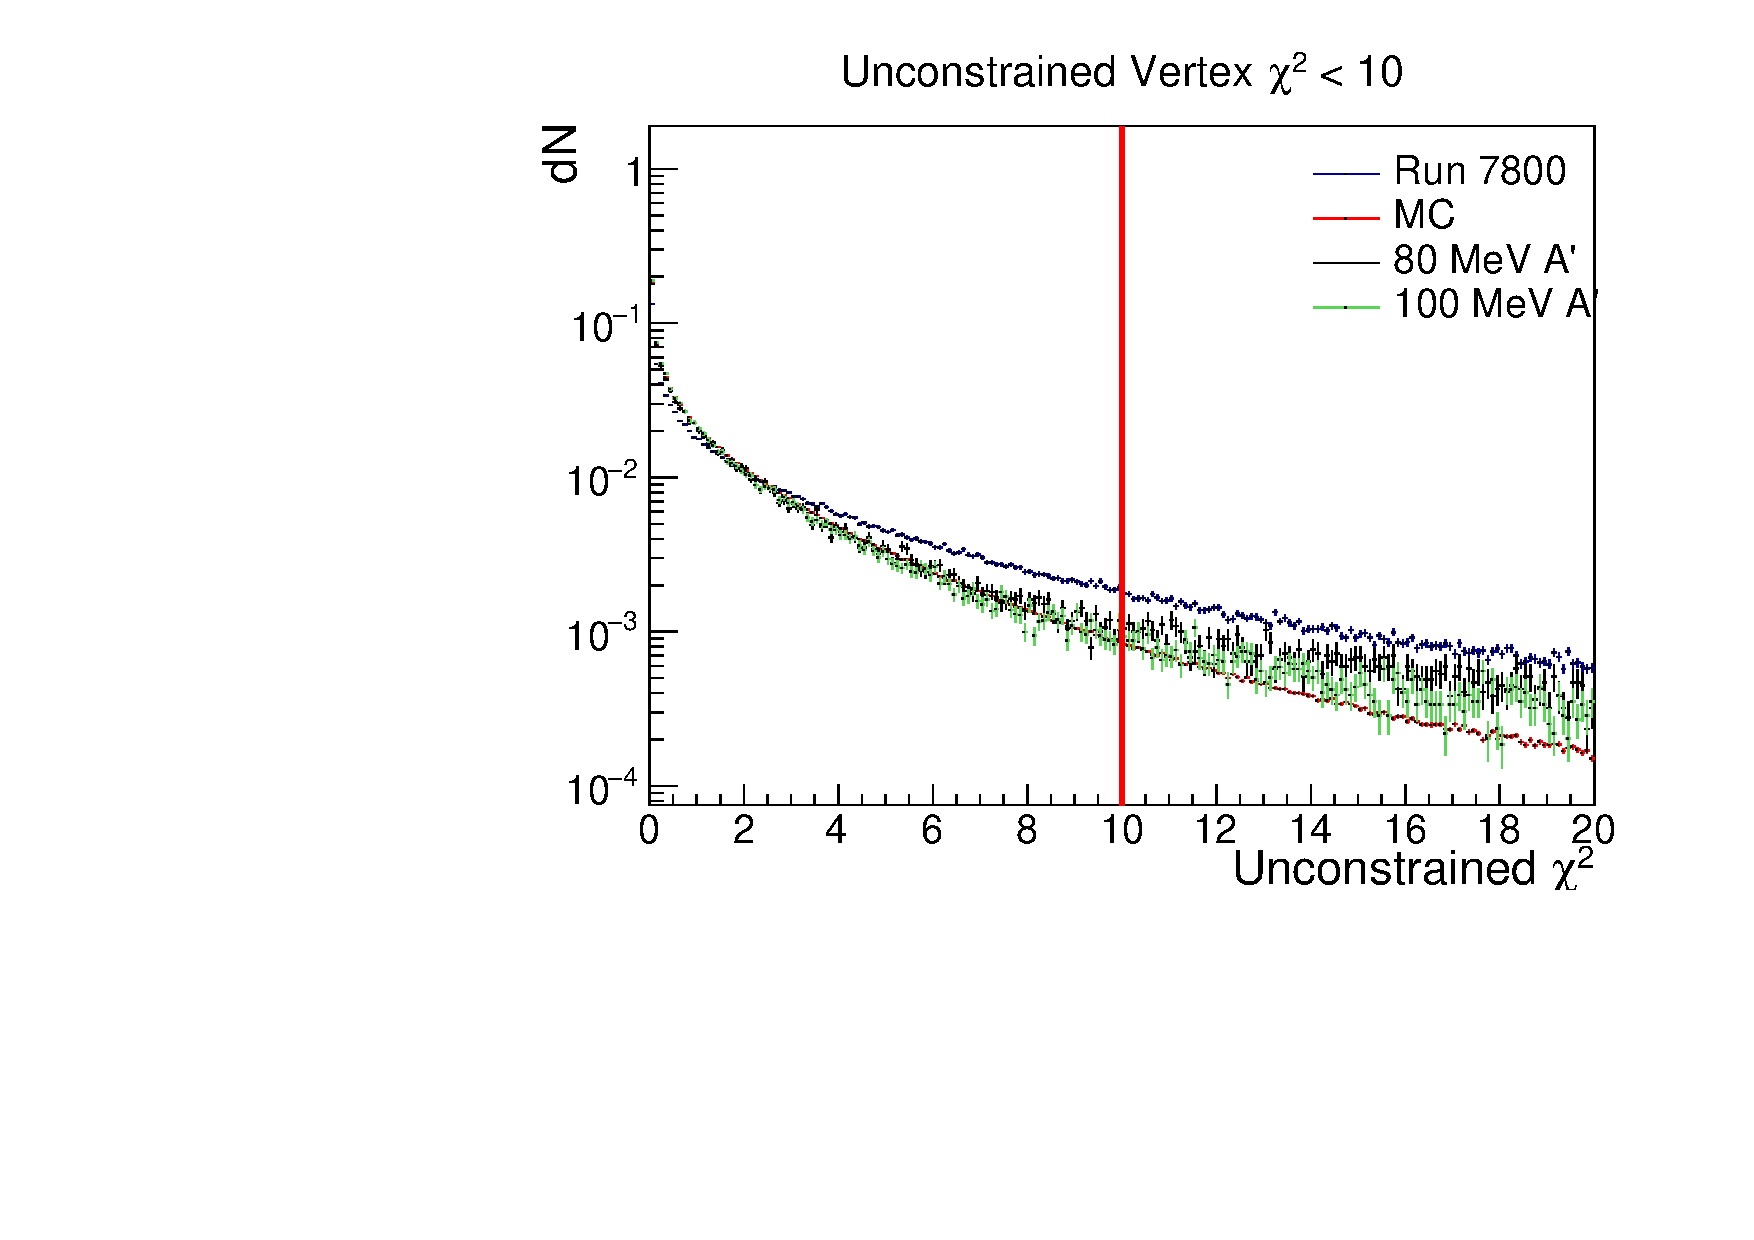
\includegraphics[width=.45\textwidth]{figs/recon/pre_uncChisq.pdf}
    \caption{%Left: A cluster time difference cut between electrons and positrons is placed at 1.45 ns to eliminate accidentals from other beam bunches (Hall B bunches are spaced at 2 ns). Right: 
    A loose cut on the unconstrained vertex fit $\chi_{unc}$ is placed at 10 to eliminate poorly reconstructed V0s that can incorrectly reconstruct downstream of the target. There is some mismodeling for the cluster time resolution, and there is some mismodeling in the vertex quality.}
    \label{fig:pre_clT_uncChisq2}
\end{figure}

\clearpage

A summary of the Preselection cuts applied to the reconstructed vertices is presented in Table \ref{tab:preselection}. % while in Table \ref{tab:cutflowPresel} the cutflow and the cut efficiency on various samples for MC simulation are shown. 
Fig. \ref{fig:preselection} shows a comparison of data and MC for preselected events while Fig. \ref{fig:pre_cutflow_z} - Fig. \ref{fig:pre_cutflow_p} show the cutflows of the preselection. At this stage, there is a significant mismatch in the tails of the vertex distribution between data and MC which become important when analyzing the prompt backgrounds that reconstruct at large $z$ in the signal region. However, once a tighter selection is applied in Sec. \ref{sec:apvertexcuts}, the agreement is much more reasonable. This initial selection is then used as a basic comparison of $\epem$ rates and kinematic shapes between data and MC, and events will later have stricter requirements to further reduce prompt backgrounds that reconstruct significantly downstream of the target.

\begin{figure}[!ht] 
    \centering
    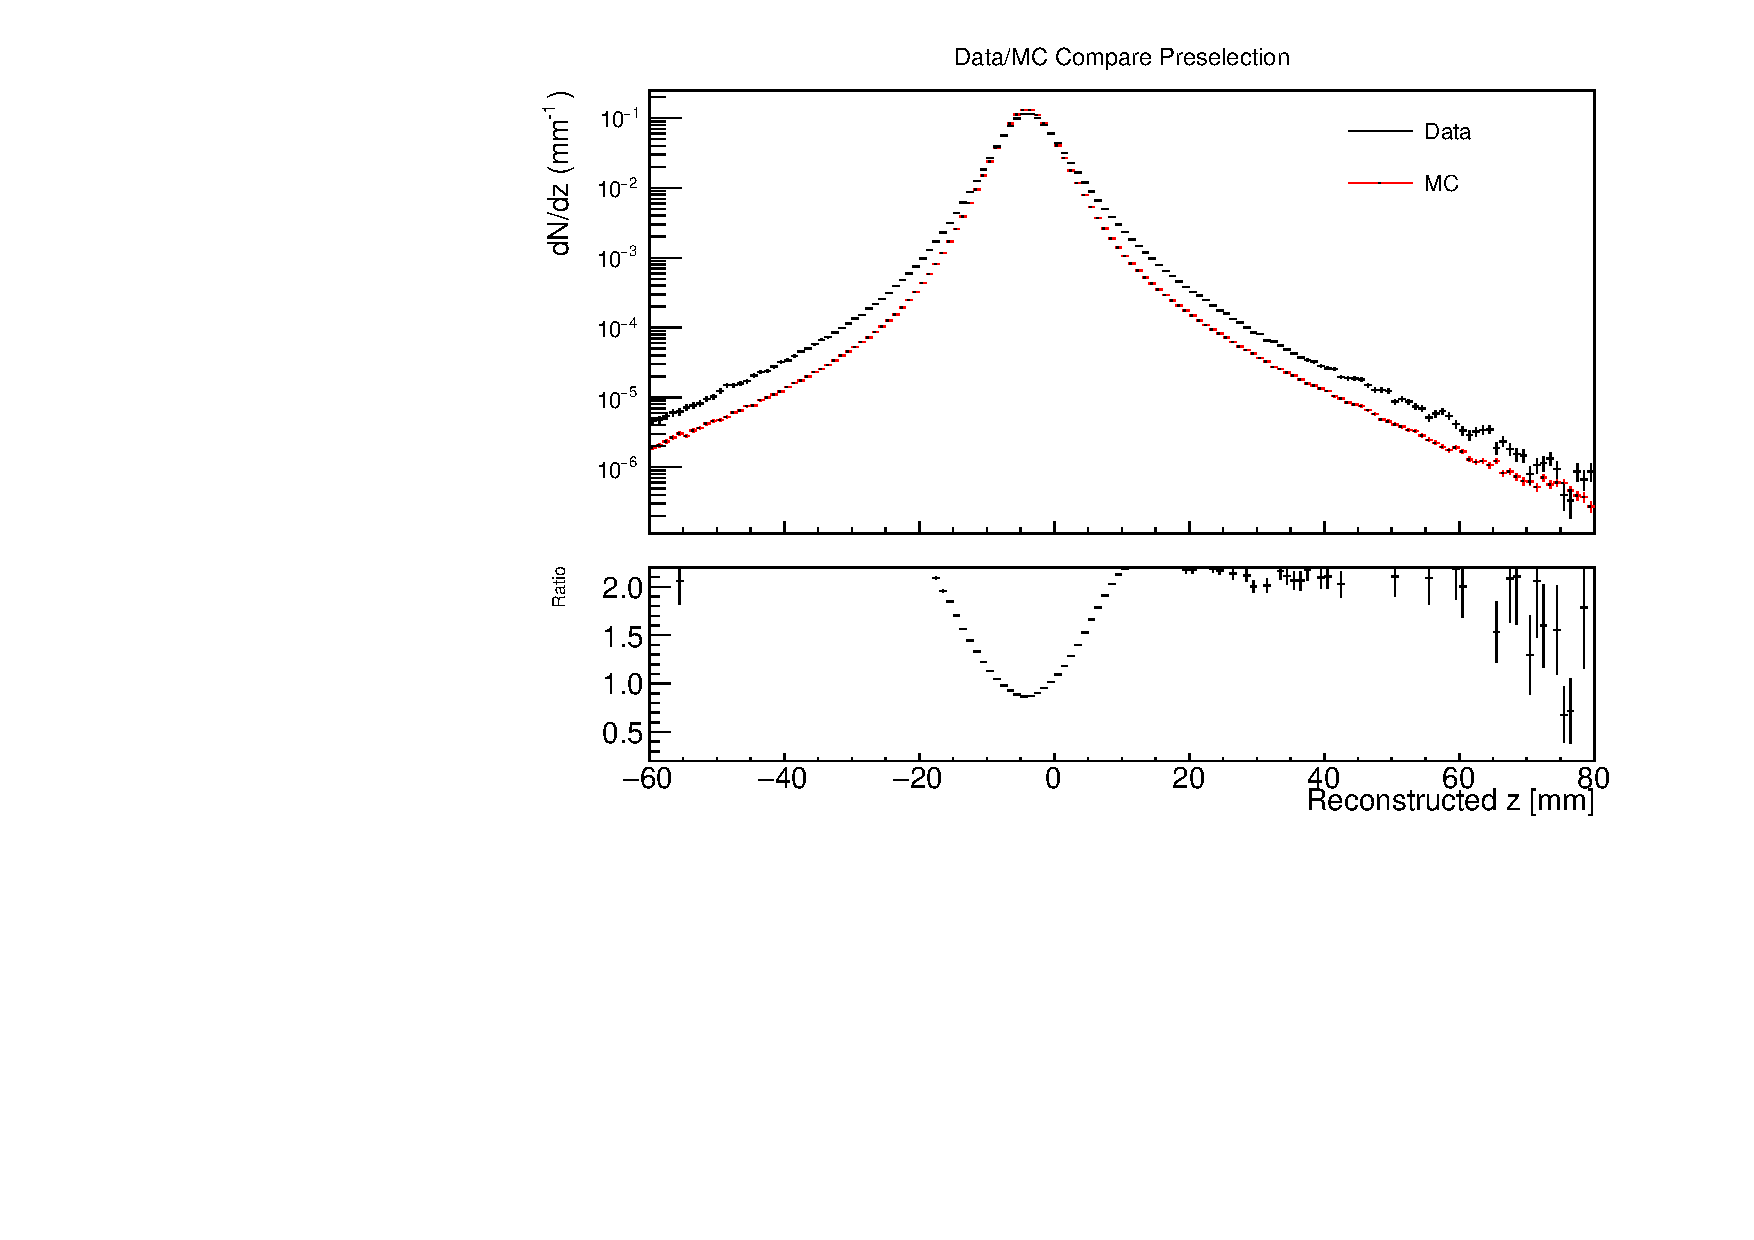
\includegraphics[width=.85\textwidth]{figs/recon/preselection_compare.pdf}
    \caption{
     Comparison of 10\% Data and tritrig-wab-beam for preselected events.
    }
    \label{fig:preselection}
\end{figure} 

\begin{figure}[t]
    \centering
    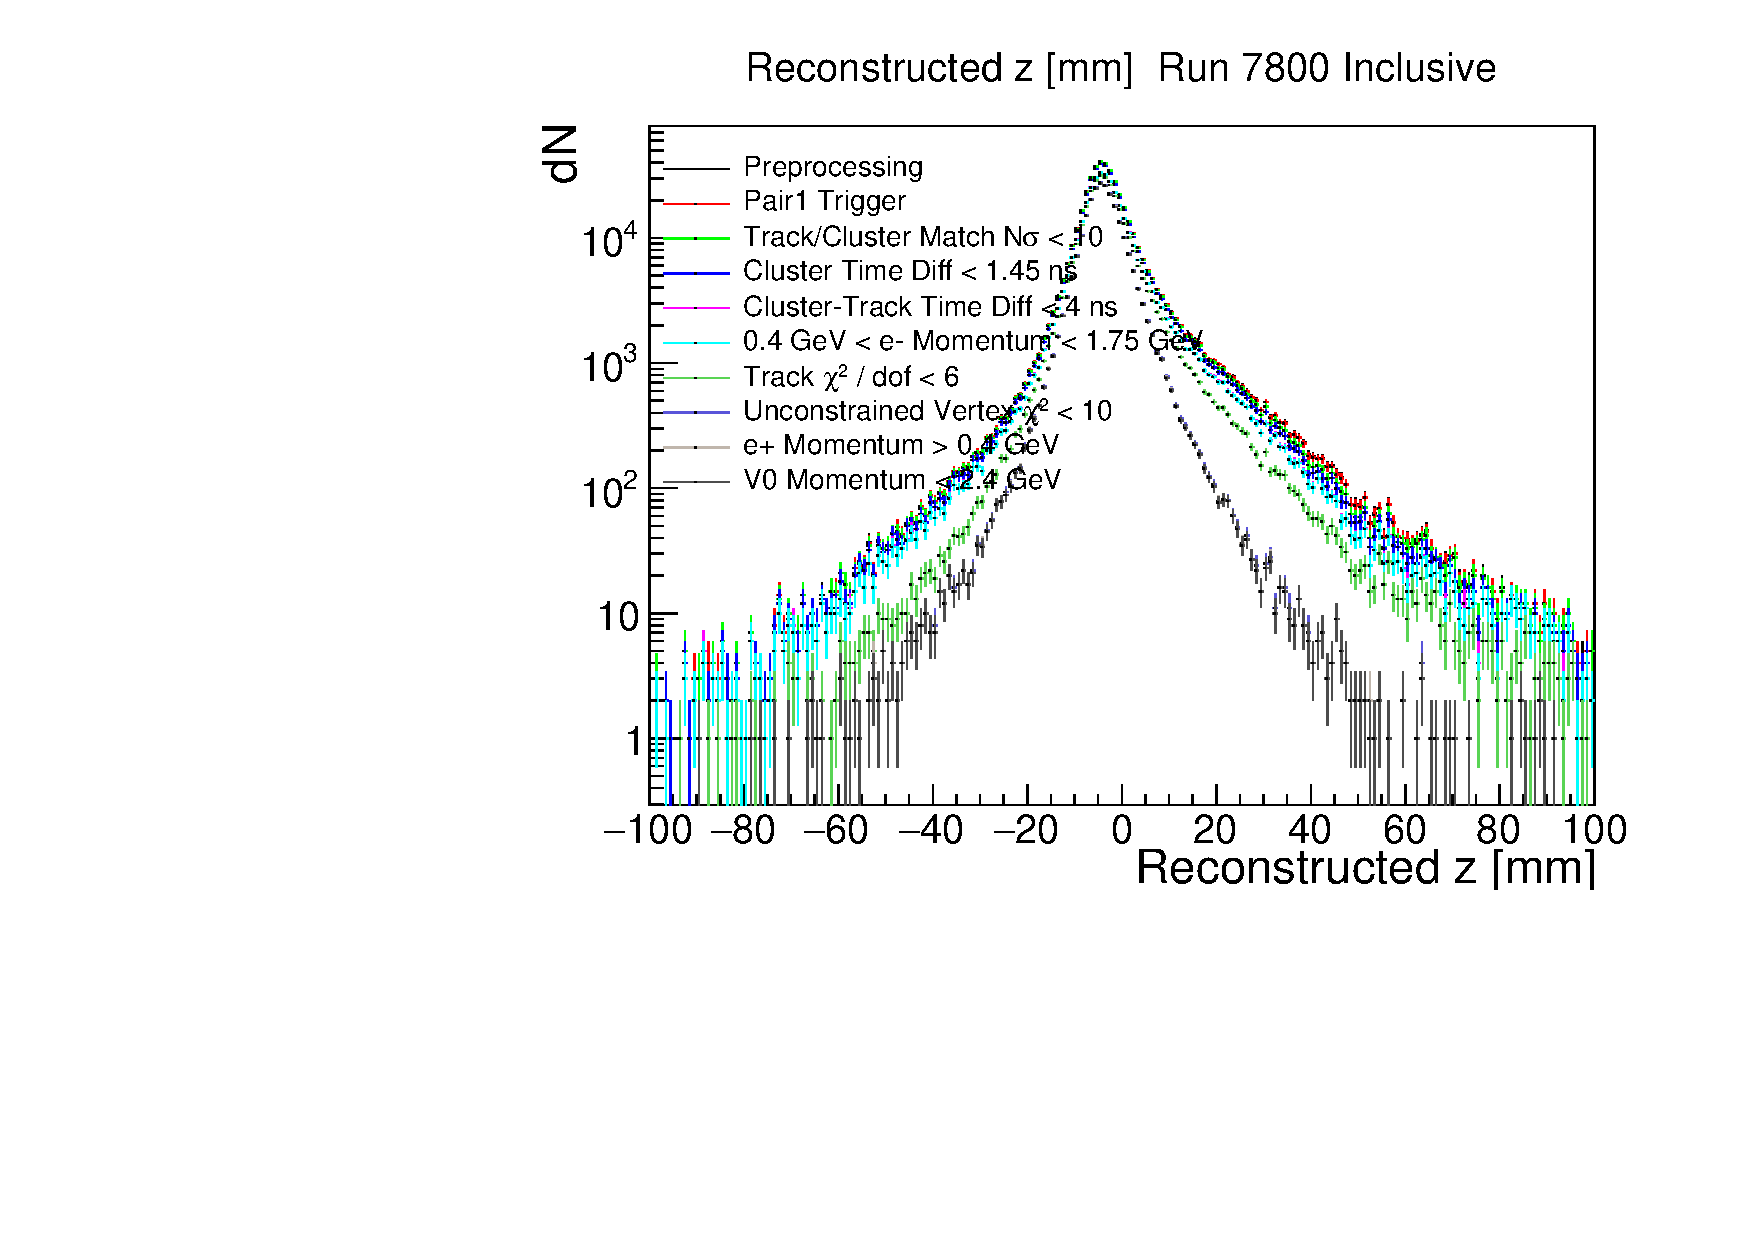
\includegraphics[width=.45\textwidth]{figs/recon/pre_cutflow_data.pdf}
    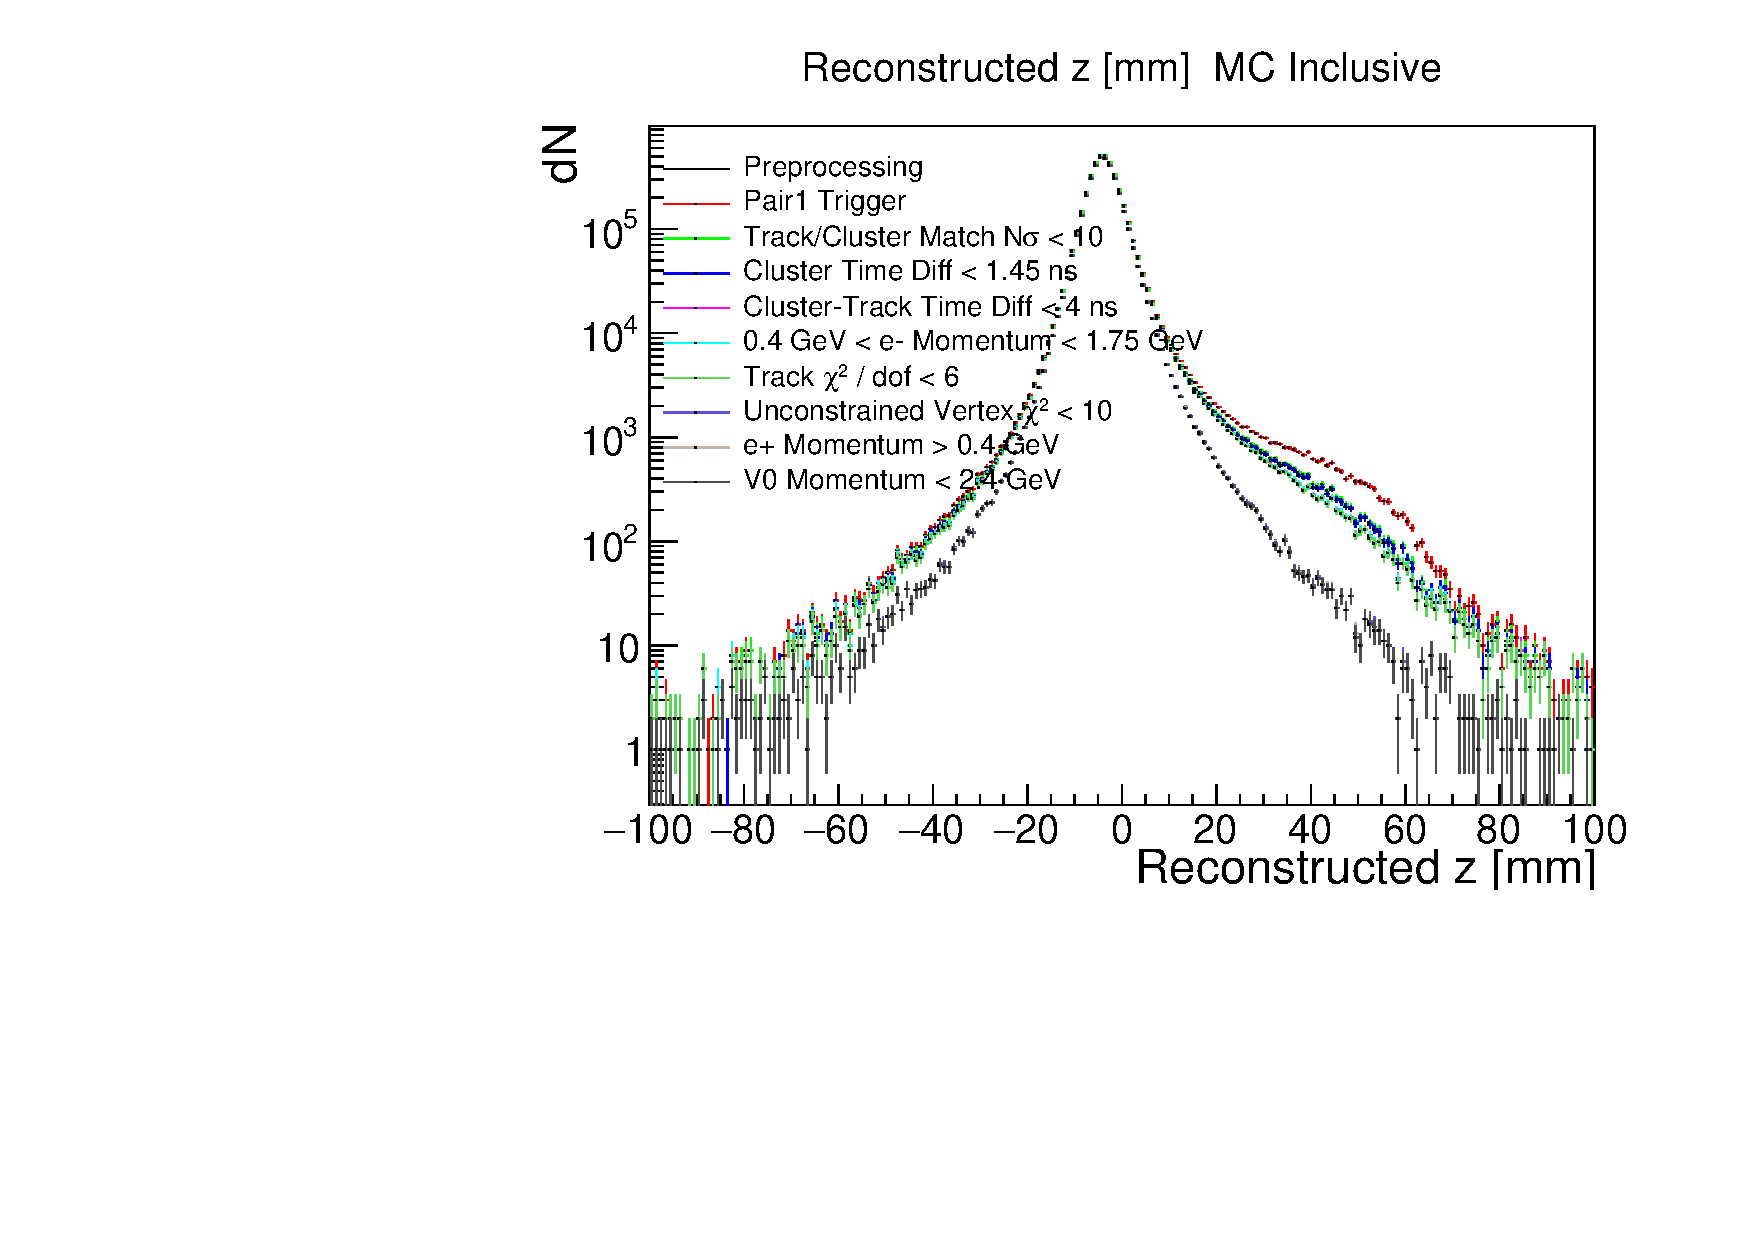
\includegraphics[width=.45\textwidth]{figs/recon/pre_cutflow_mc.pdf}
    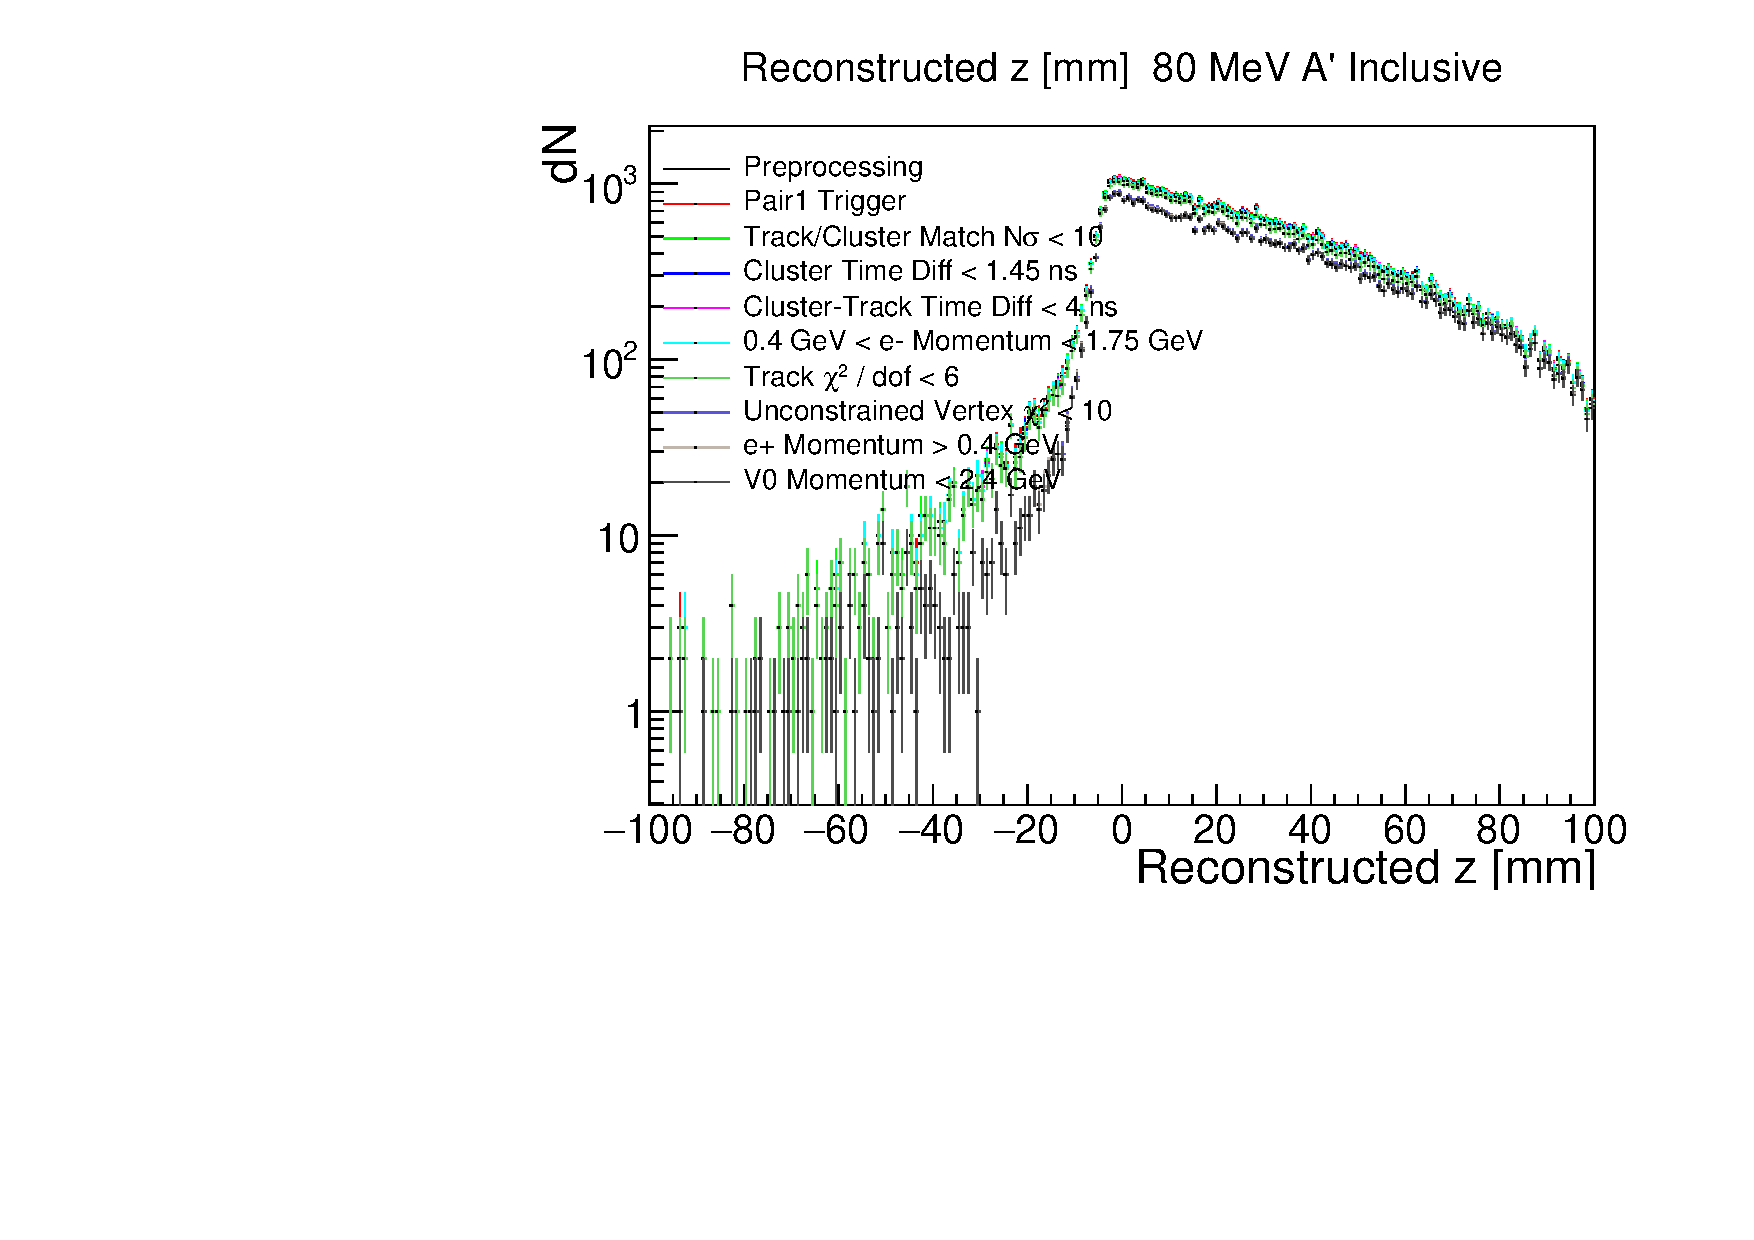
\includegraphics[width=.45\textwidth]{figs/recon/pre_cutflow_ap80.pdf}
    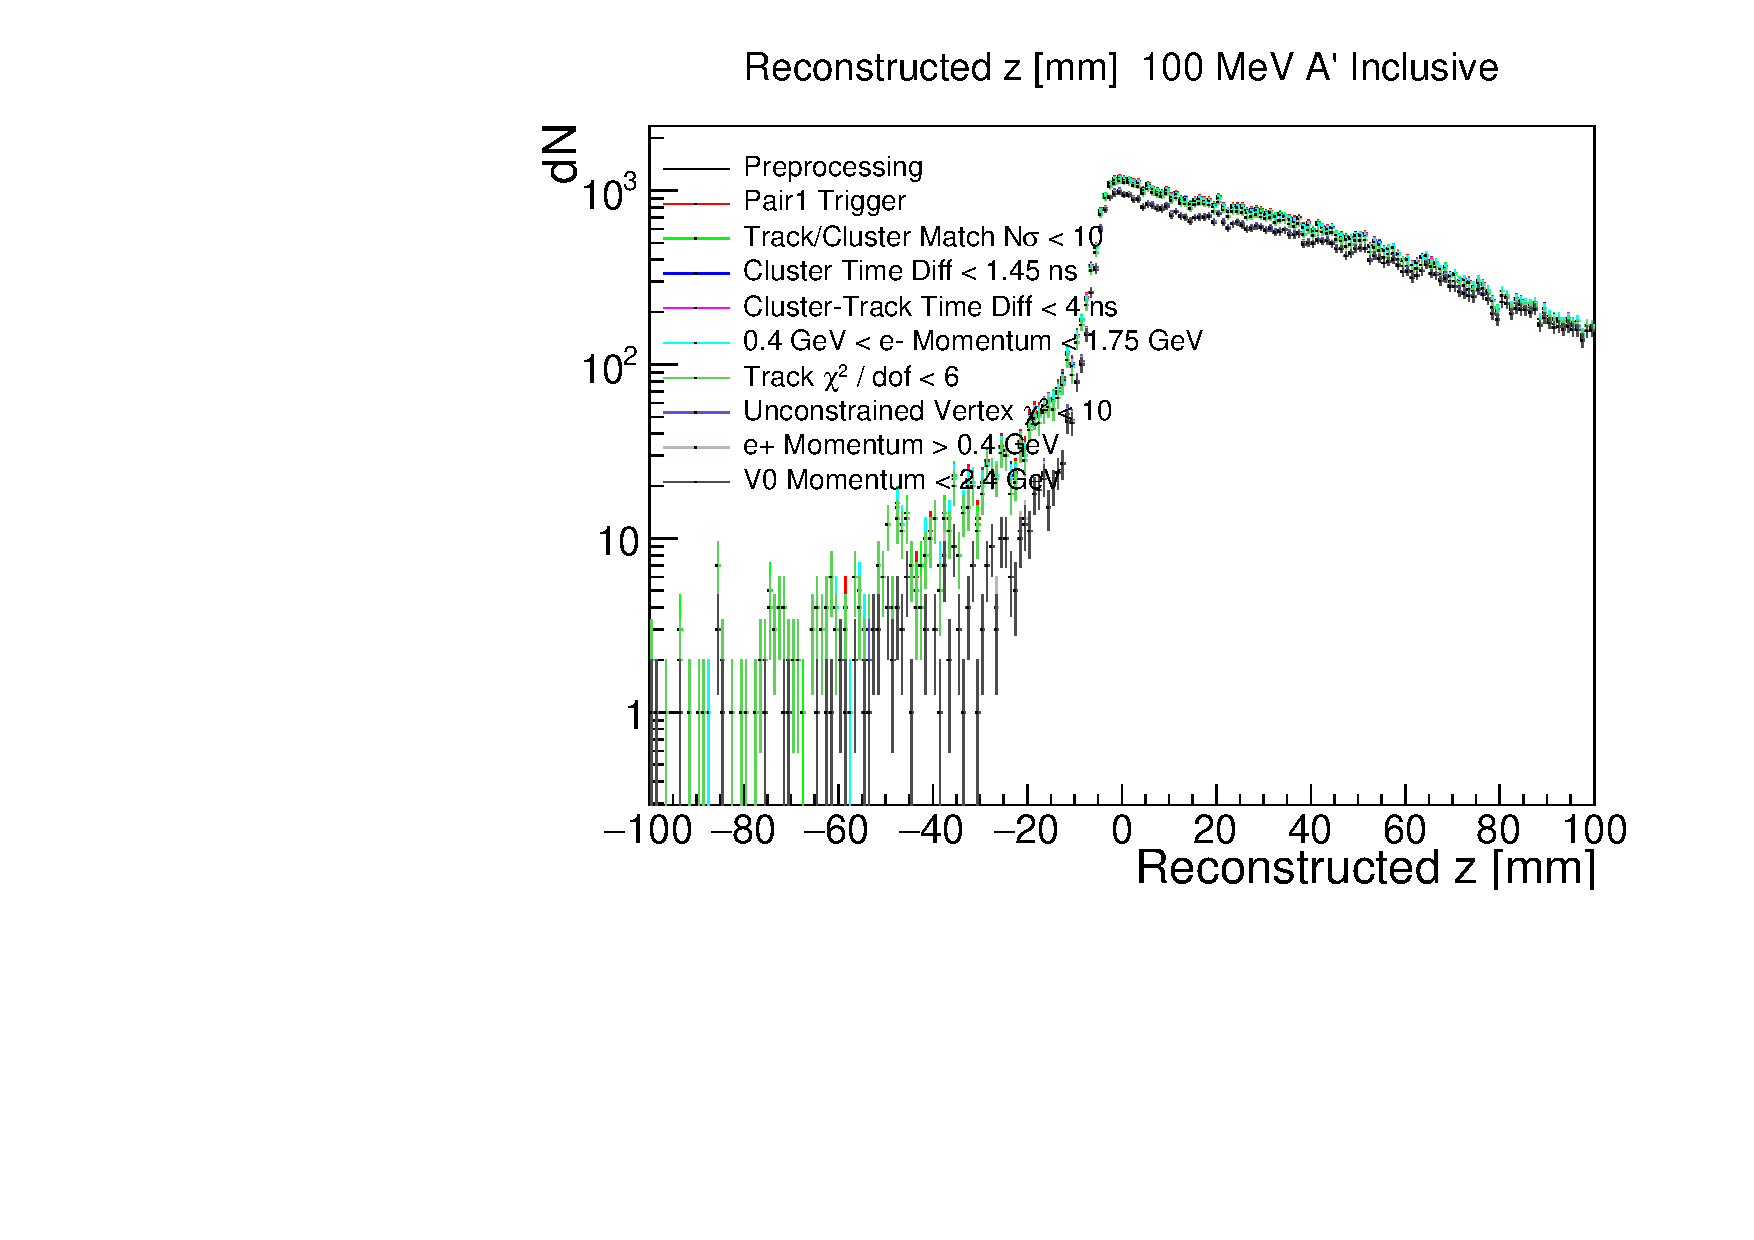
\includegraphics[width=.45\textwidth]{figs/recon/pre_cutflow_ap100.pdf}
    \caption{Preselection cutflow as a function of reconstructed $z$. Top Left: Run 7800 in data. Top Right: a fraction of the tritrig-wab-beam sample. Bottom Left: 80 MeV displaced $A'$s. Bottom Right: 100 MeV displaced $A'$s.}
    \label{fig:pre_cutflow_z}
\end{figure}

\begin{figure}[t]
    \centering
    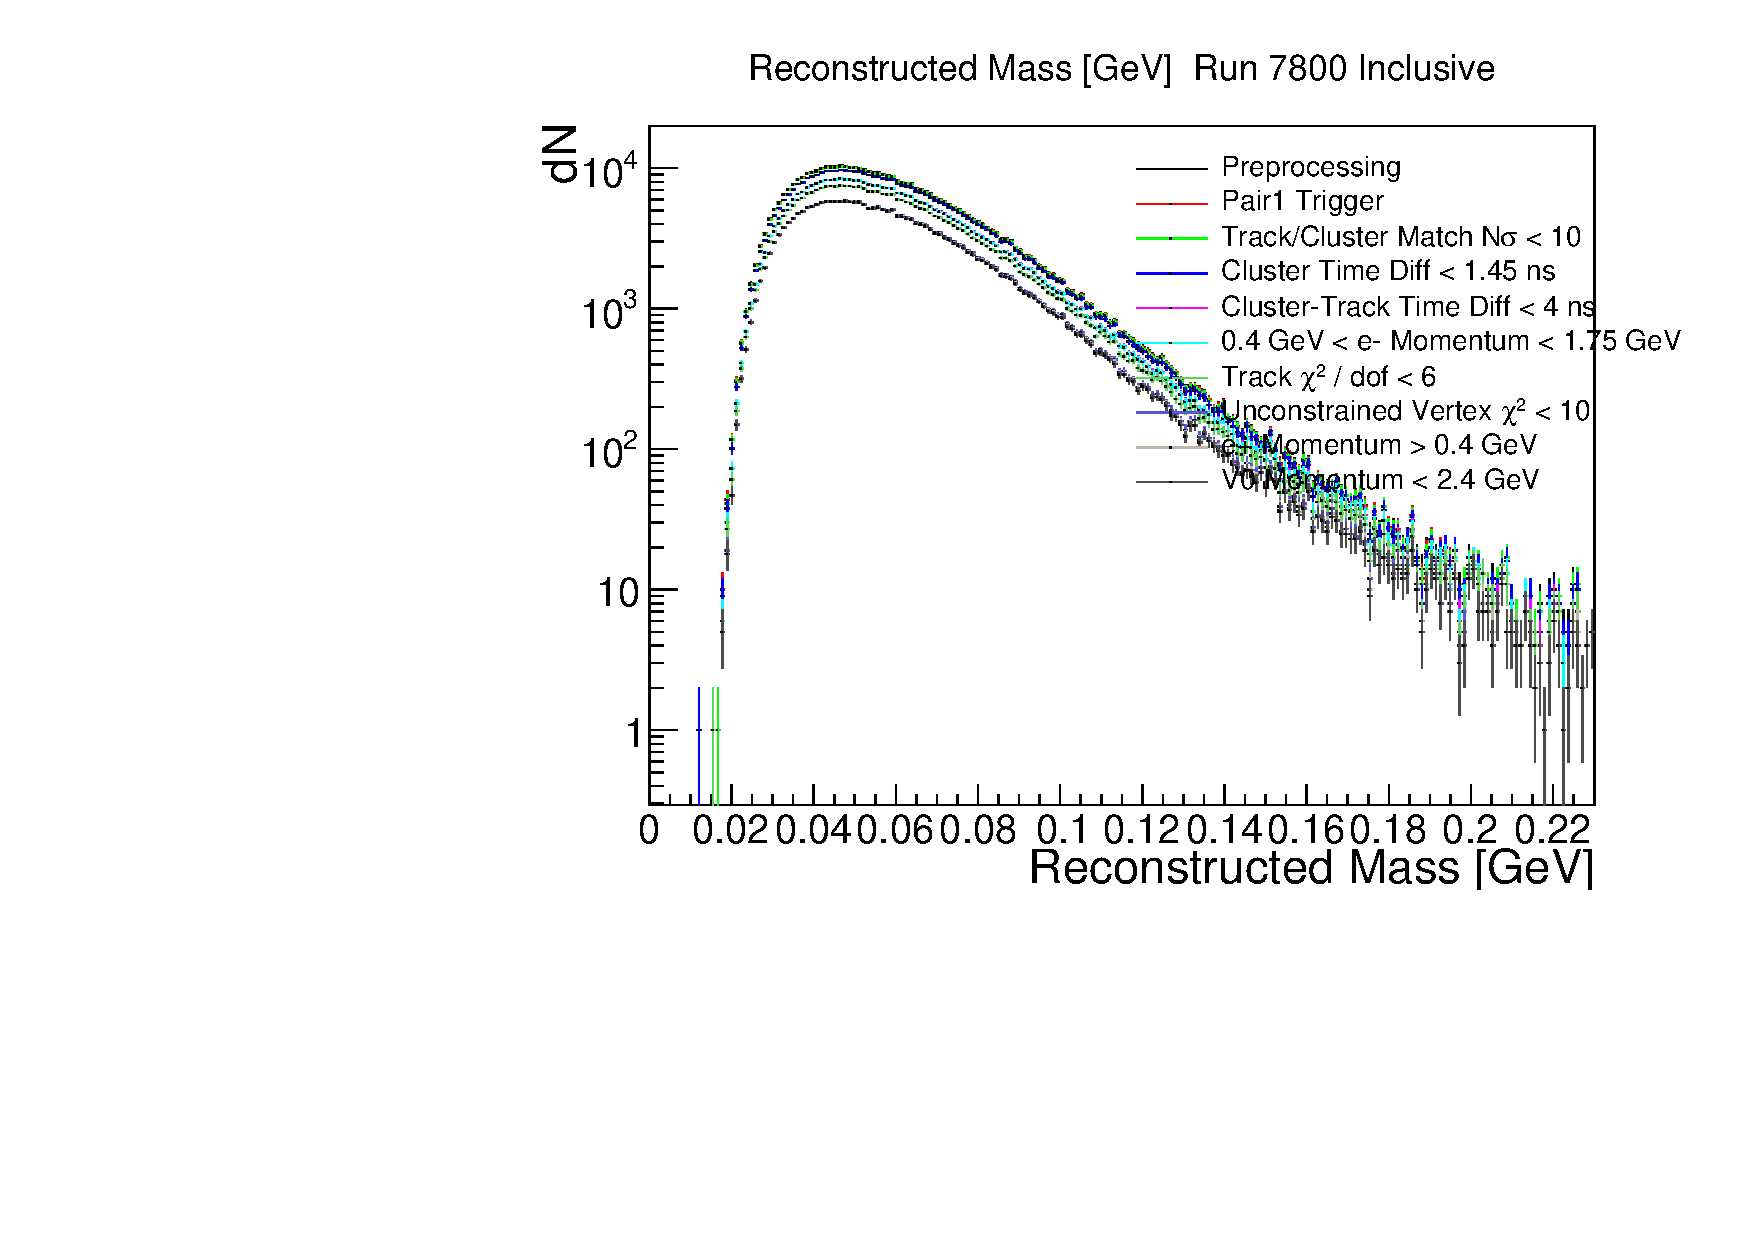
\includegraphics[width=.45\textwidth]{figs/recon/pre_cutflow_uncM_data.pdf}
    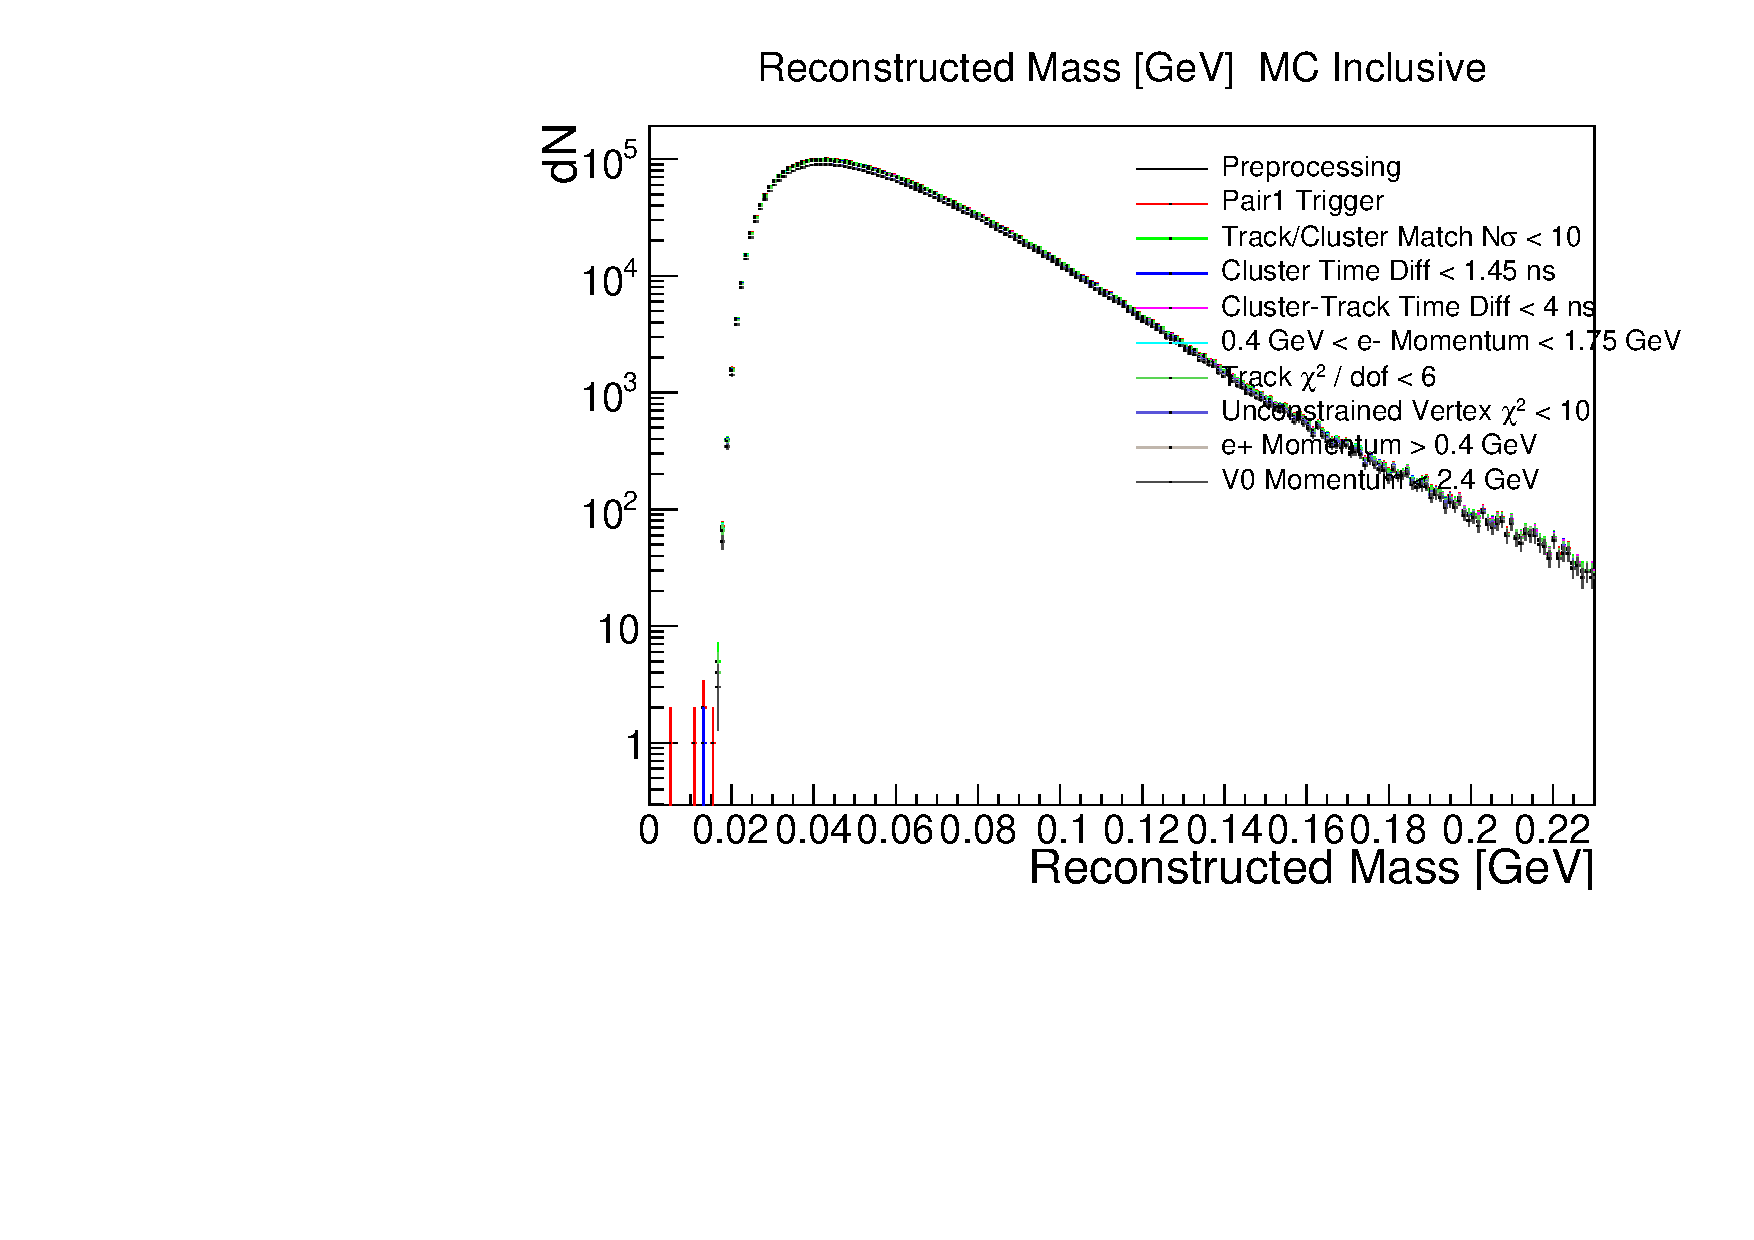
\includegraphics[width=.45\textwidth]{figs/recon/pre_cutflow_uncM_mc.pdf}
    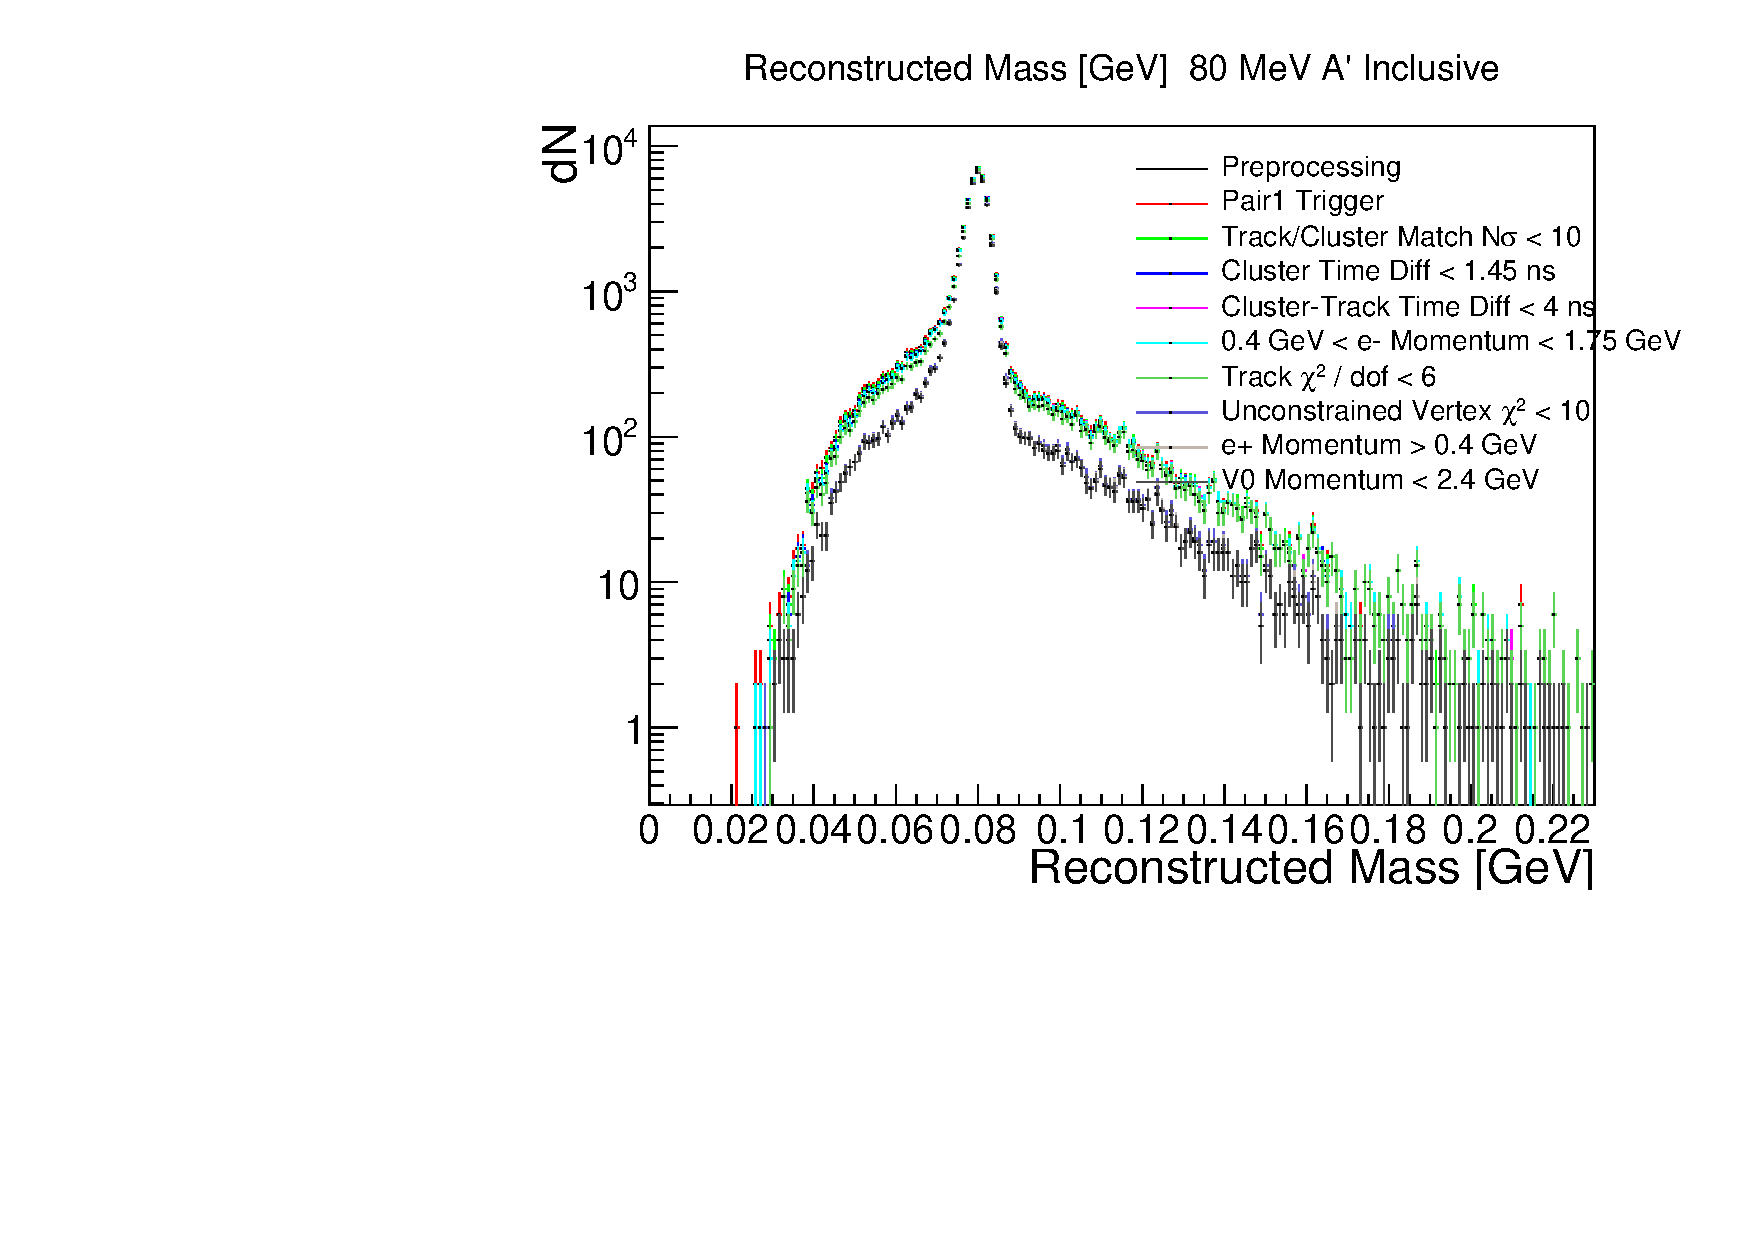
\includegraphics[width=.45\textwidth]{figs/recon/pre_cutflow_uncM_ap80.pdf}
    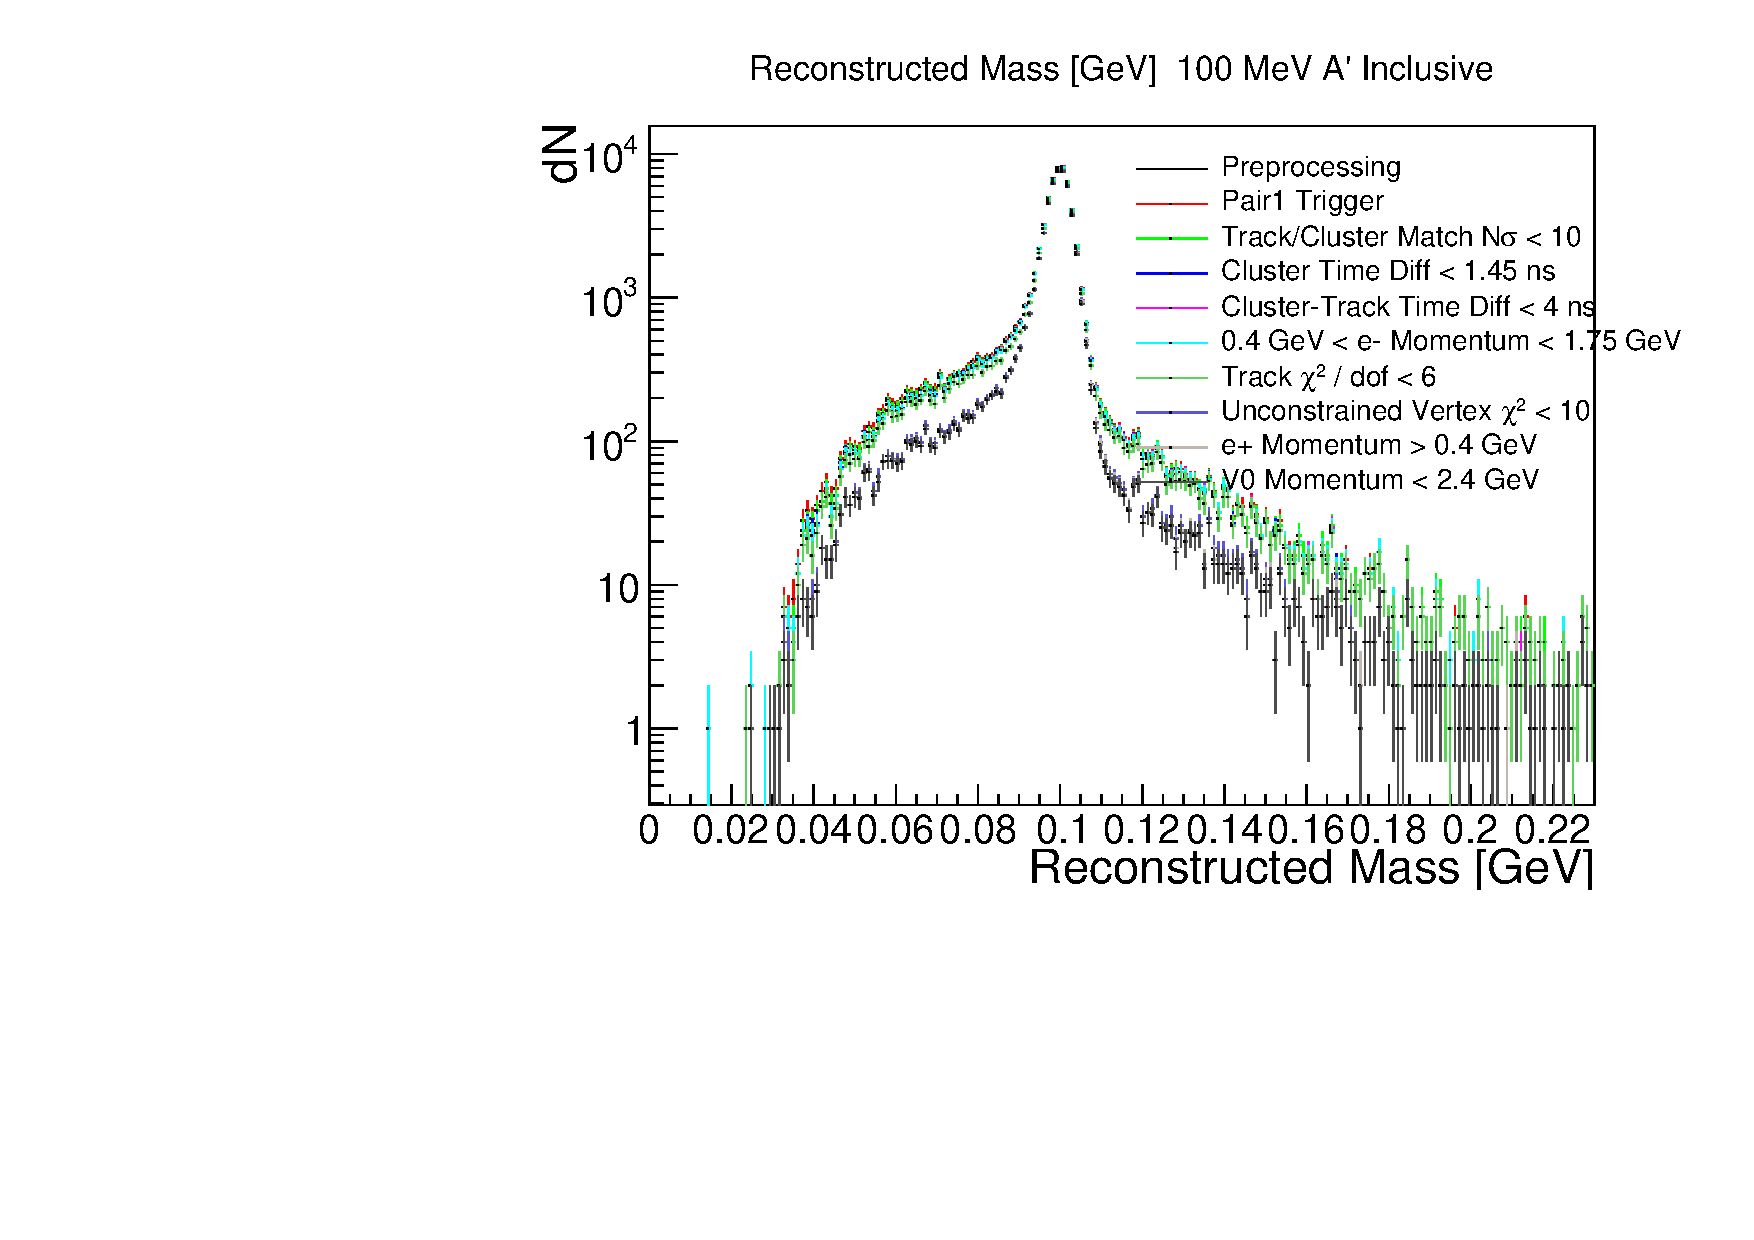
\includegraphics[width=.45\textwidth]{figs/recon/pre_cutflow_uncM_ap100.pdf}
    \caption{Preselection cutflow as a function of reconstructed mass. Top Left: Run 7800 in data. Top Right: a fraction of the tritrig-wab-beam sample. Bottom Left: 80 MeV displaced $A'$s. Bottom Right: 100 MeV displaced $A'$s.}
    \label{fig:pre_cutflow_m}
\end{figure}

\begin{figure}[t]
    \centering
    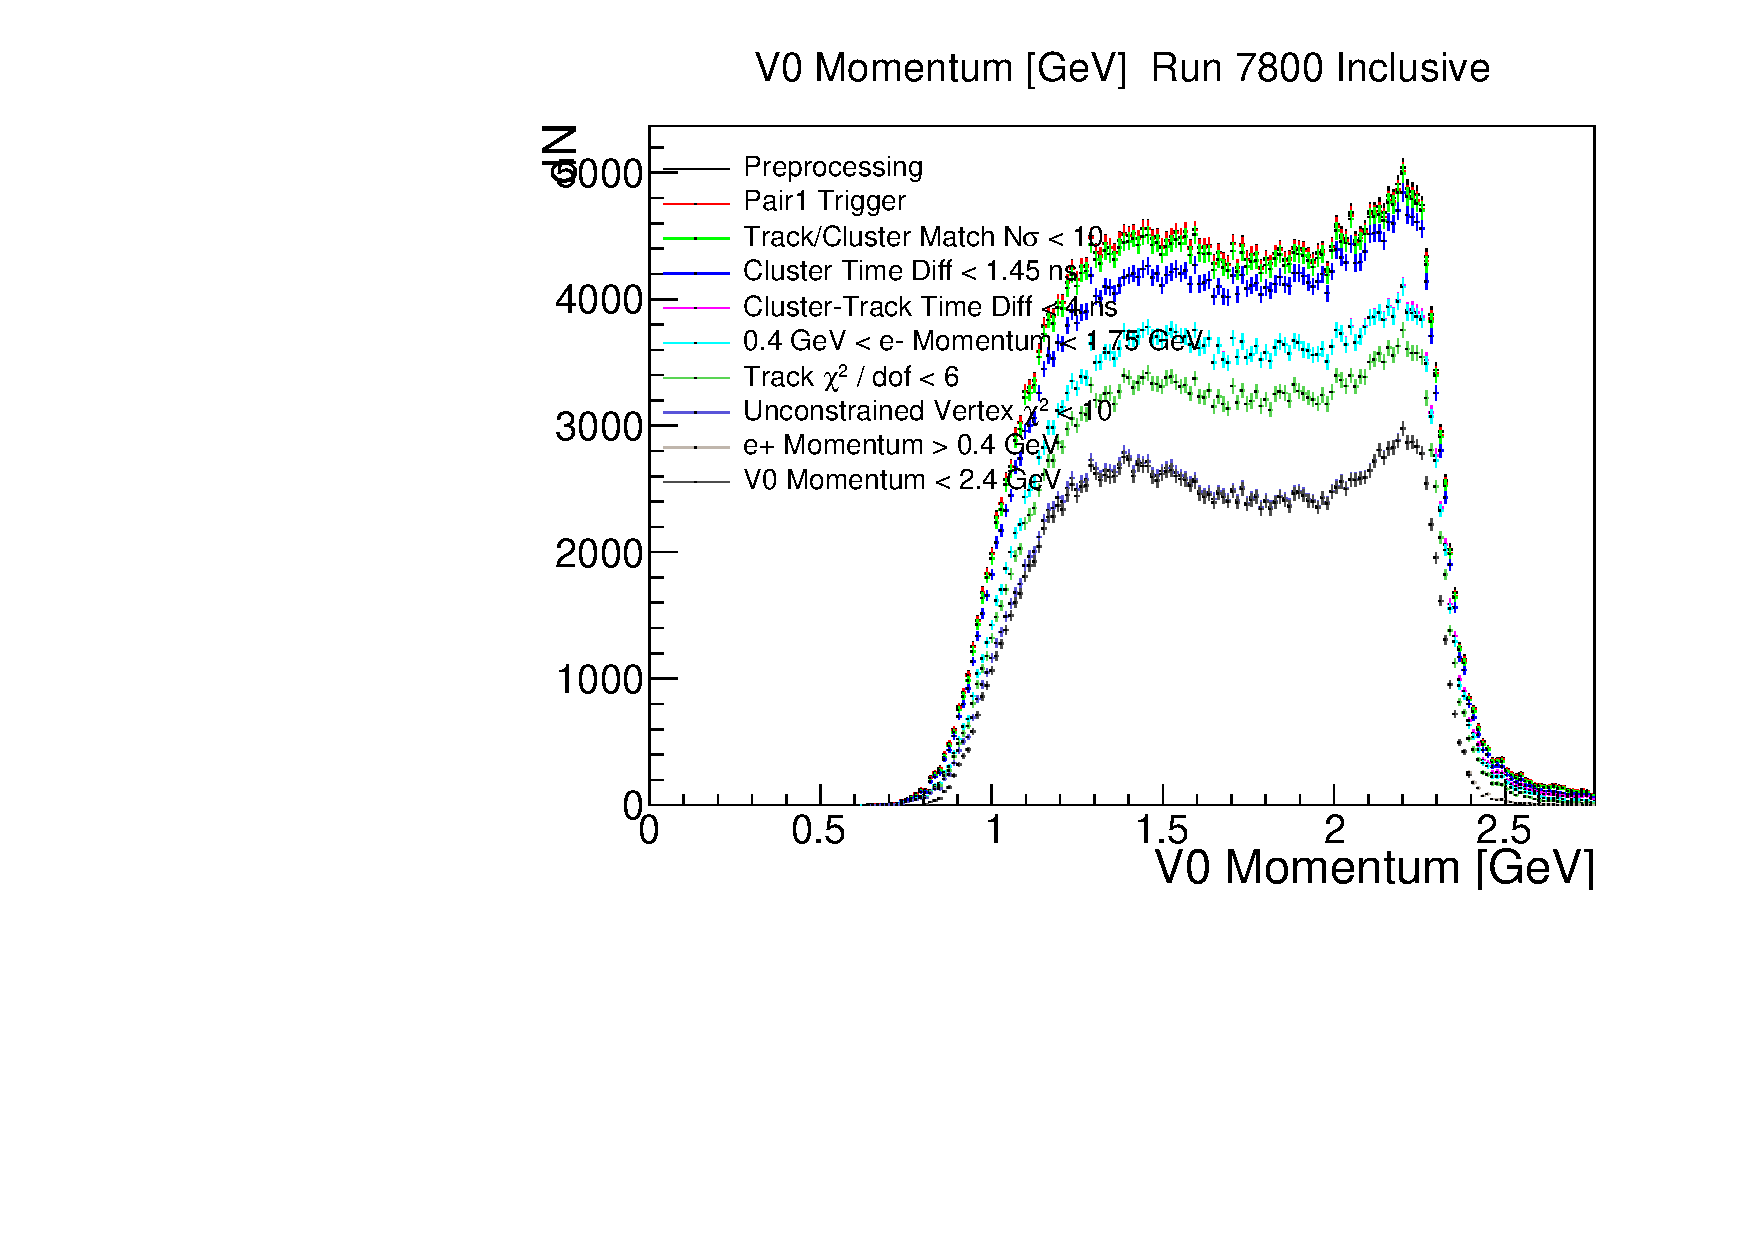
\includegraphics[width=.45\textwidth]{figs/recon/pre_cutflow_uncP_data.pdf}
    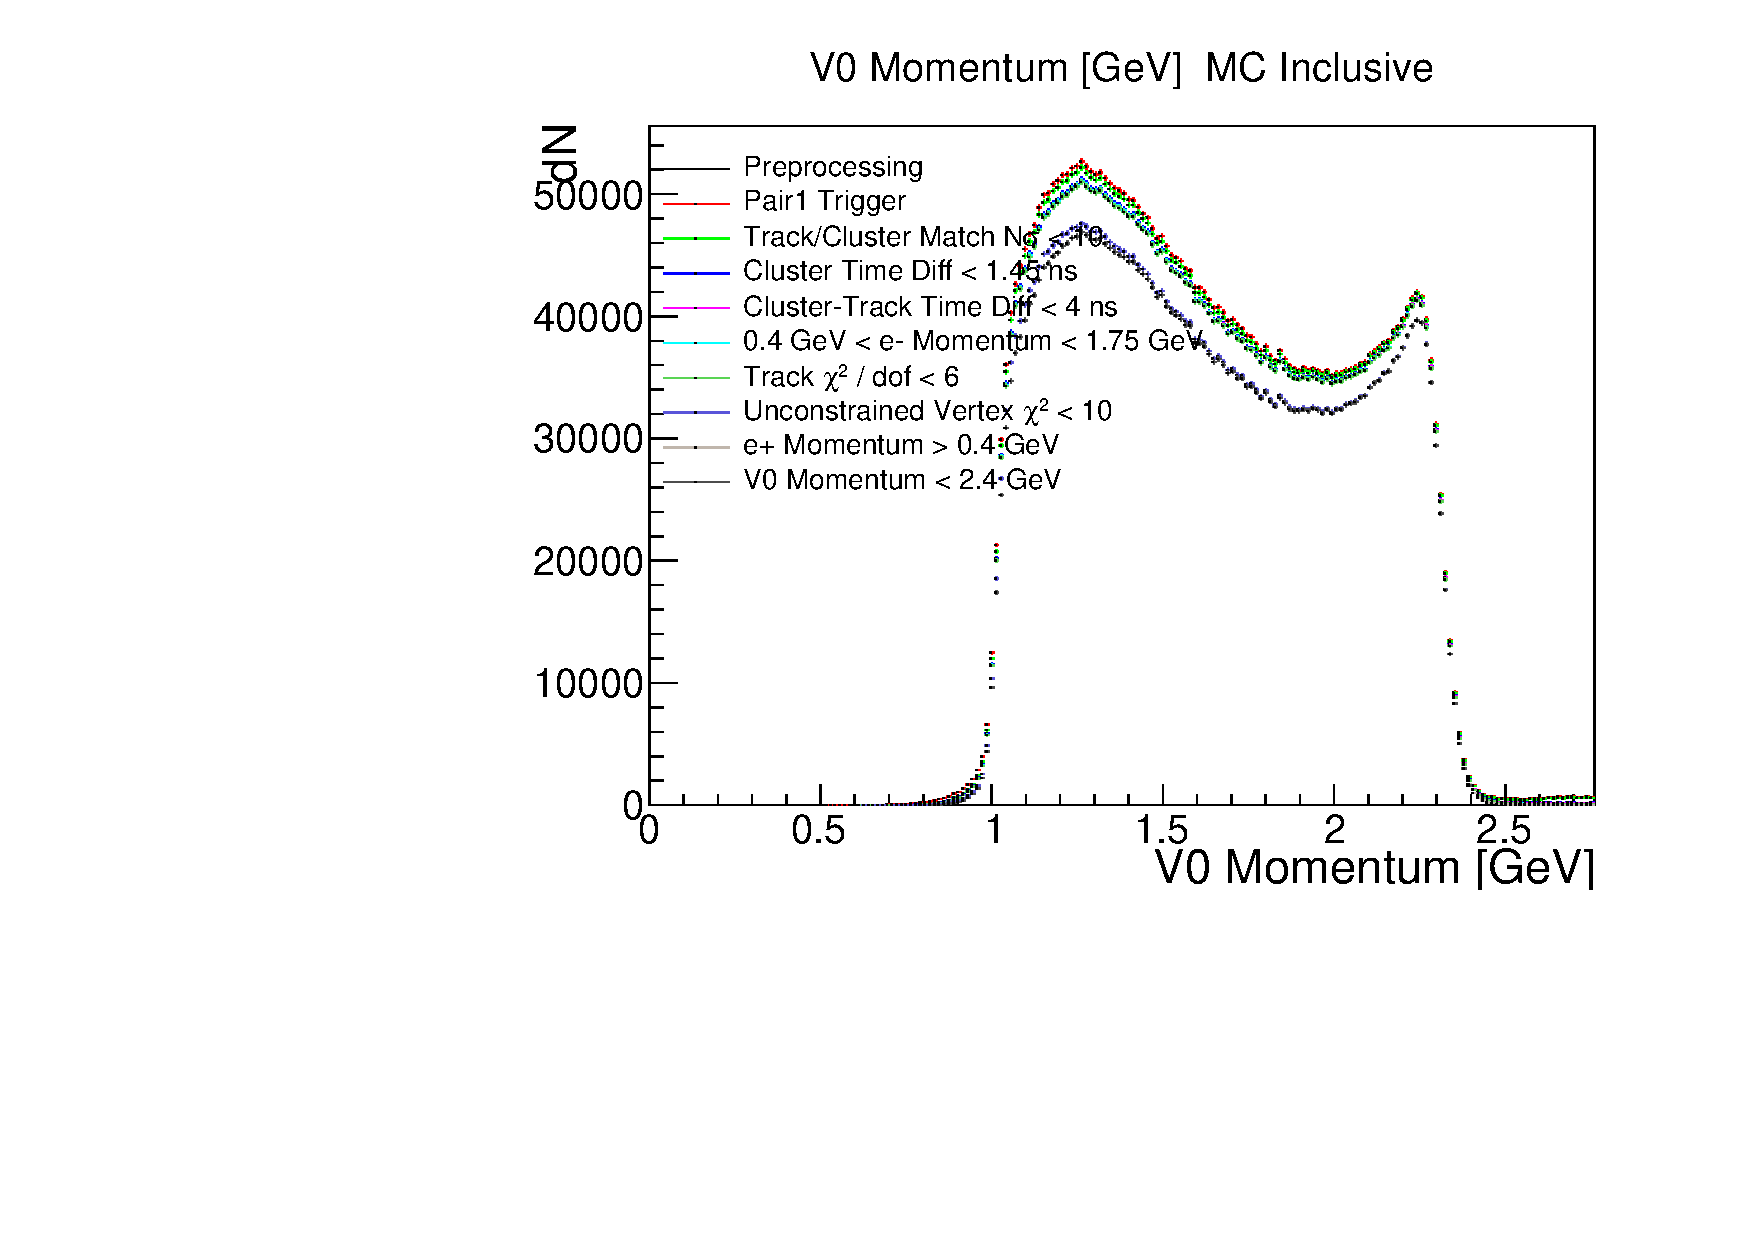
\includegraphics[width=.45\textwidth]{figs/recon/pre_cutflow_uncP_mc.pdf}
    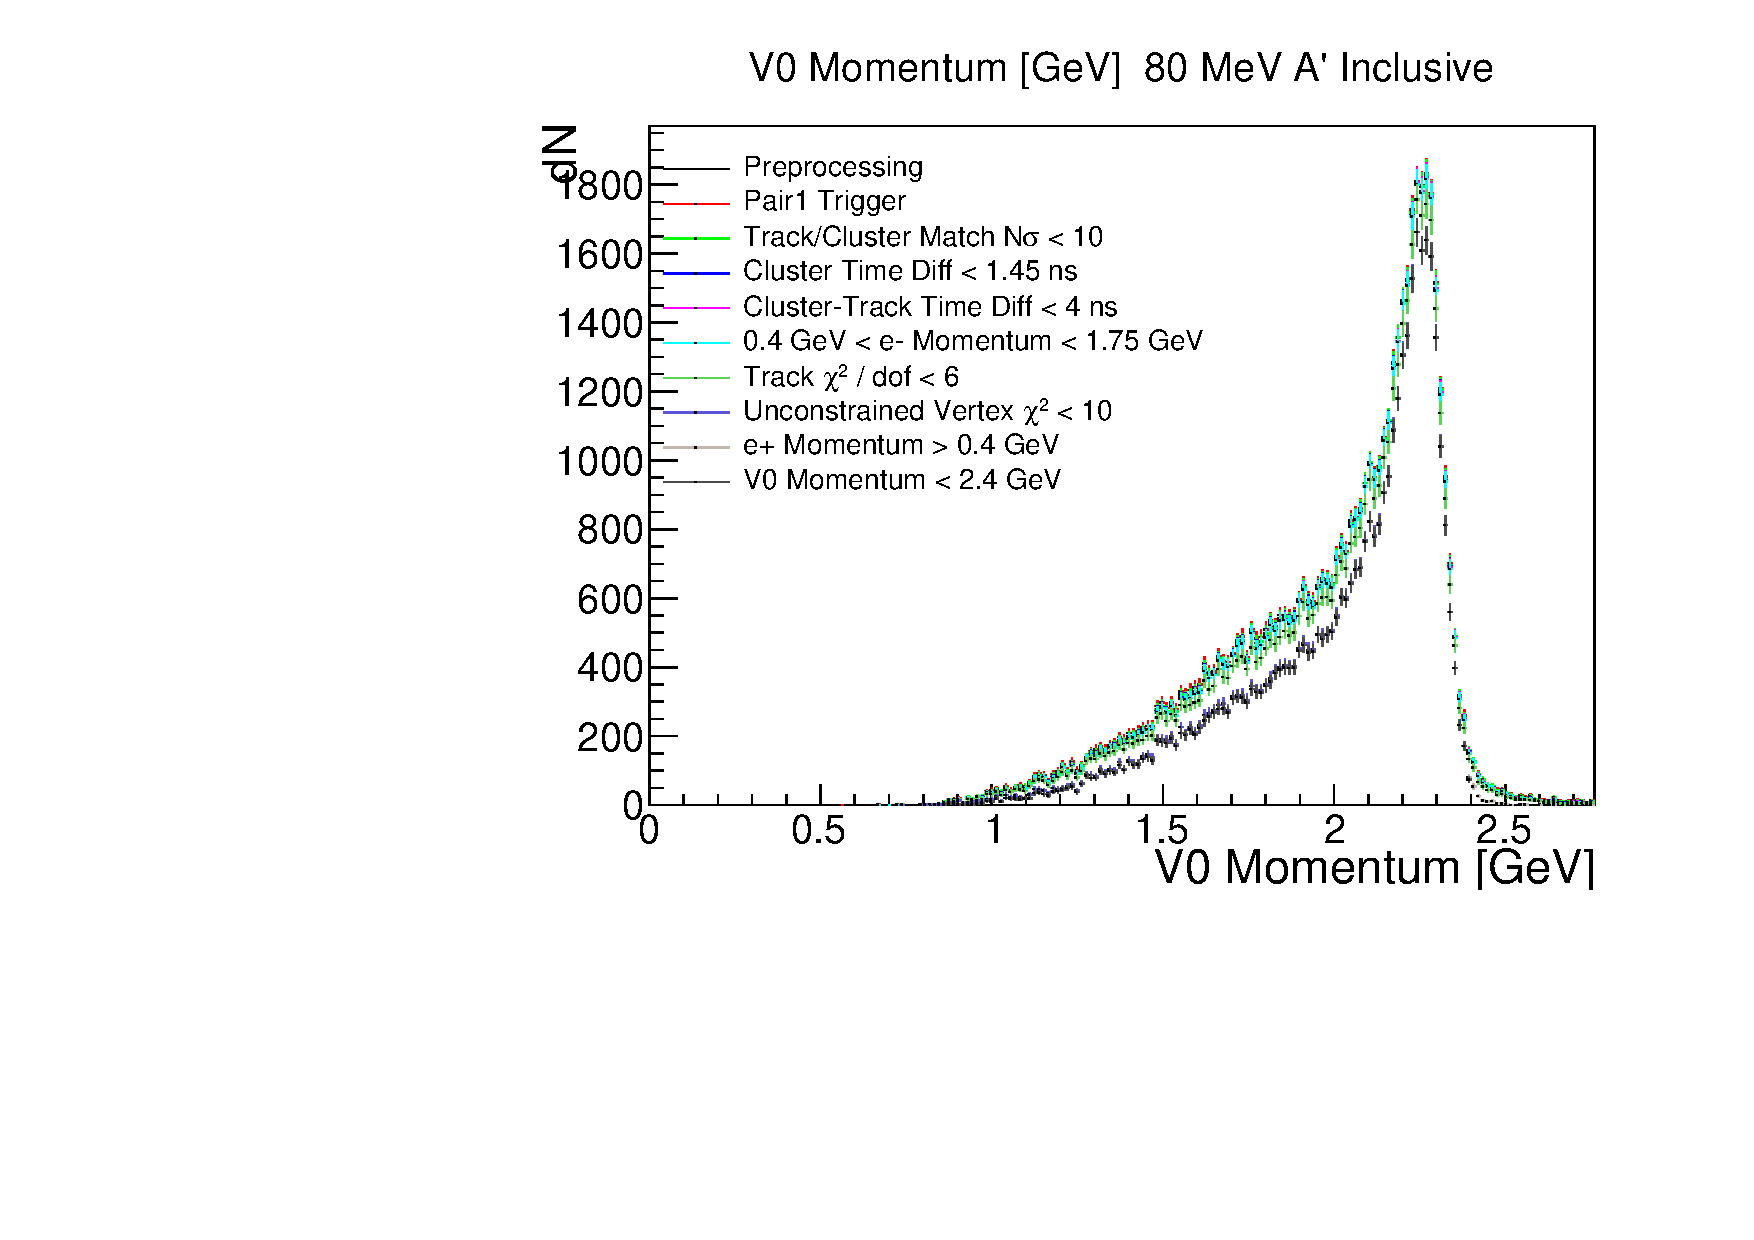
\includegraphics[width=.45\textwidth]{figs/recon/pre_cutflow_uncP_ap80.pdf}
    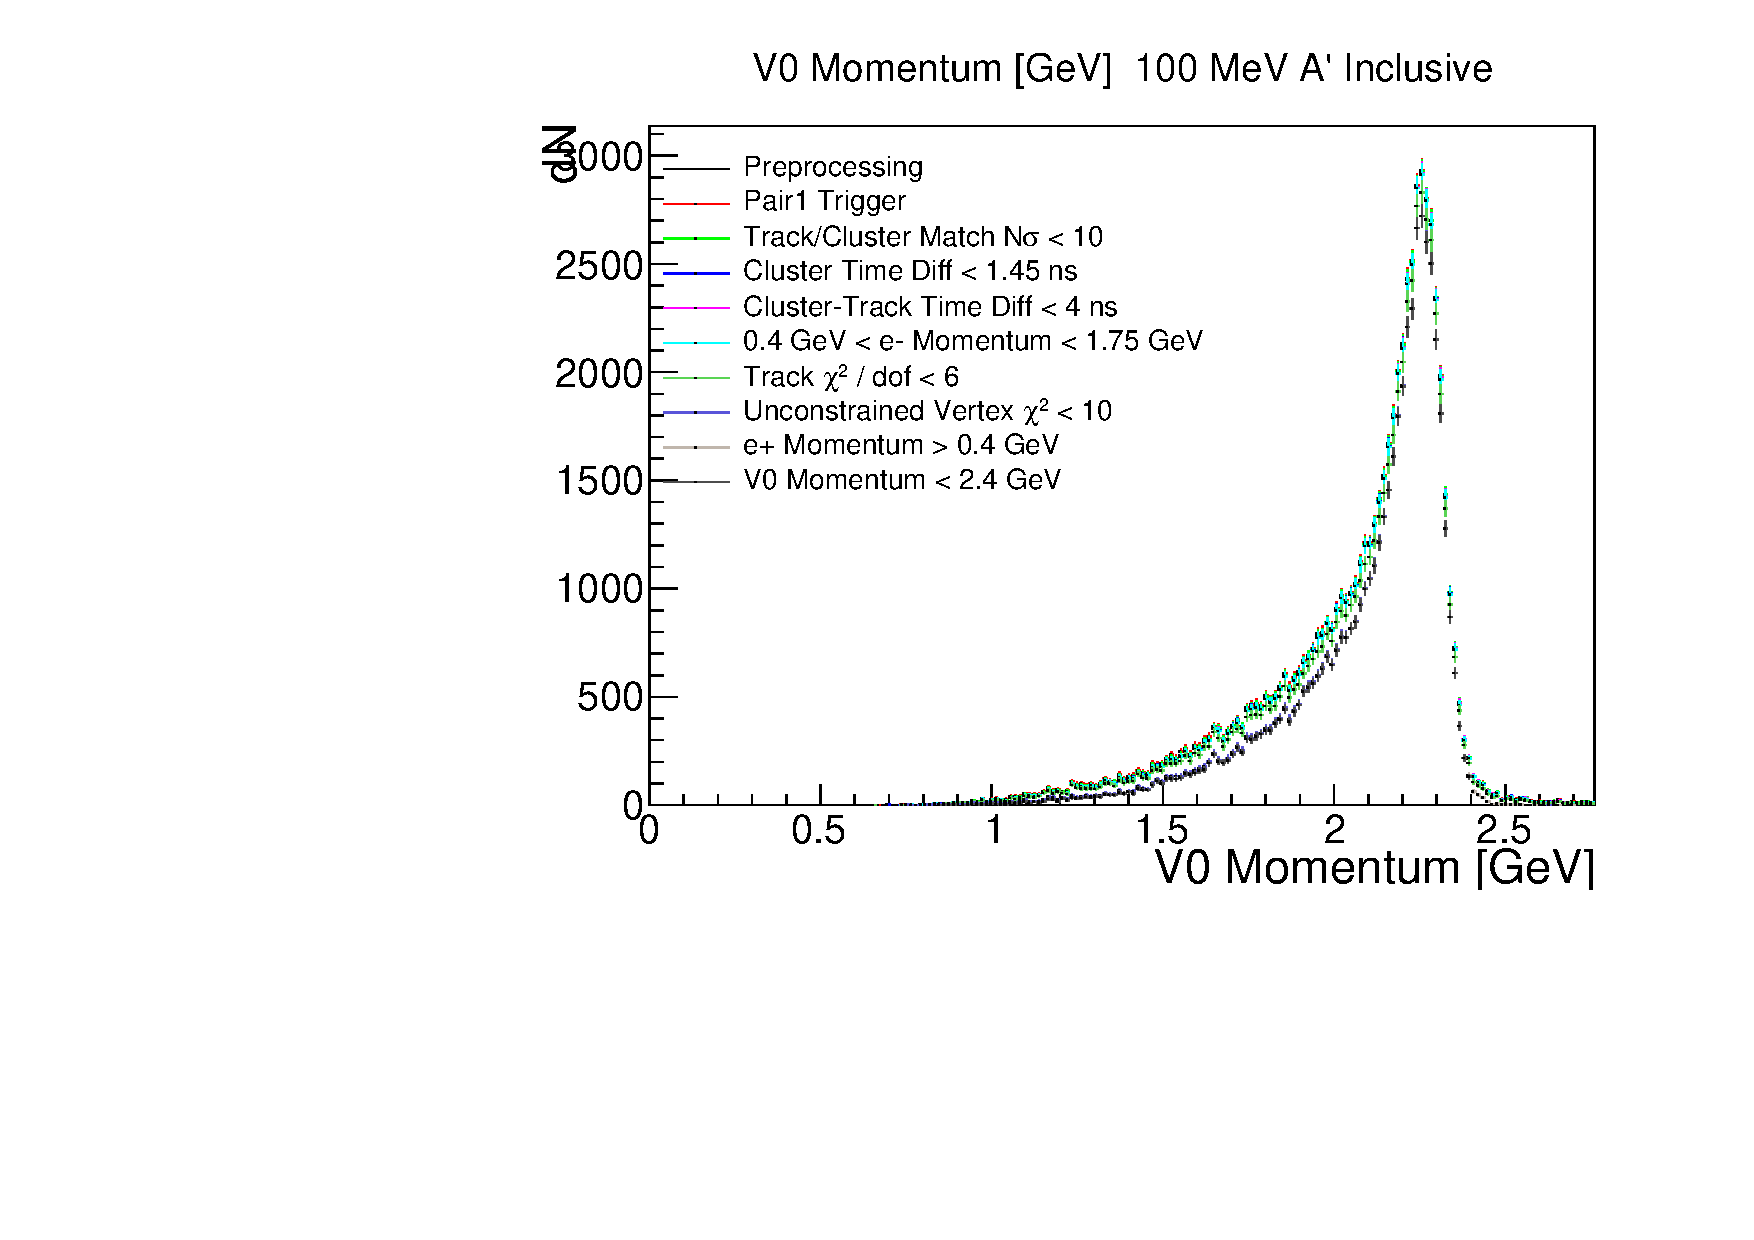
\includegraphics[width=.45\textwidth]{figs/recon/pre_cutflow_uncP_ap100.pdf}
    \caption{Preselection cutflow as a function of reconstructed V0 momentum. Top Left: Run 7800 in data. Top Right: a fraction of the tritrig-wab-beam sample. Bottom Left: 80 MeV displaced $A'$s. Bottom Right: 100 MeV displaced $A'$s. The $\aprime$ invariant mass spectrum contains tails far away from its mass which is mostly a result of the recoil electron occasionally reconstructing with a daughter positron.}
    \label{fig:pre_cutflow_p}
\end{figure}

%\begin{table}[t]
%\centering
%\tabcolsep=0.09cm
%\begin{tabular}{lrlrlrlrl}

% \hline
%                                         &        data & $\epsilon_{tot}$   &    tridents & $\epsilon_{tot}$   &   WAB & $\epsilon_{tot}$   &    AP & $\epsilon_{tot}$   \\
%\hline
% no-cuts                                 & 2.65672e+07 & --                 & 8.05260e+06 & --                 & 31921 & --                 & 55952 & --                 \\
% Trigger Pair1                           & 2.65022e+07 & 0.998              & 0           & 0.0                &     0 & 0.0                &     0 & 0.0                \\
% $e^{-} \Delta_{d}(trk,clu)<10\sigma$      & 2.63041e+07 & 0.99               & 7.96627e+06 & 0.989              & 31702 & 0.993              & 55363 & 0.989              \\
% $e^{+} \Delta_{d}(trk,clu)<10\sigma$      & 2.62441e+07 & 0.988              & 7.94766e+06 & 0.987              & 31473 & 0.986              & 55251 & 0.987              \\
% $\Delta_{t}(clu_{e^{-}},clu_{e^{+}})<2$ns & 2.49811e+07 & 0.94               & 7.83282e+06 & 0.973              & 31002 & 0.971              & 54665 & 0.977              \\
% $e^{-} \Delta_{t}(trk,clu)<4$ns           & 2.26414e+07 & 0.852              & 7.78389e+06 & 0.967              & 30882 & 0.967              & 54463 & 0.973              \\
% $e^{+} \Delta_{t}(trk,clu)<4$ns           & 2.15004e+07 & 0.809              & 7.7633e+06  & 0.964              & 30440 & 0.954              & 54293 & 0.97               \\
% $p e^{-}<1.75$GeV                         & 2.14217e+07 & 0.806              & 7.75548e+06 & 0.963              & 30379 & 0.952              & 54201 & 0.969              \\
% $e^{-} Track \chi^{2}<6$                  & 2.06244e+07 & 0.776              & 7.58028e+06 & 0.941              & 29735 & 0.932              & 52652 & 0.941              \\
% $e^{+} Track \chi^{2}<6$                  & 1.9464e+07  & 0.733              & 7.42088e+06 & 0.922              & 27139 & 0.85               & 50983 & 0.911              \\
% $\chi^{2}_{unc}<10$                       & 1.53681e+07 & 0.578              & 6.9479e+06  & 0.863              & 13226 & 0.414              & 42929 & 0.767              \\
% $p_e^{-}>0.4$GeV                       & 1.5204e+07  & 0.572              & 6.88443e+06 & 0.855              & 13194 & 0.413              & 42474 & 0.759              \\
% $p_e^{+}>0.4$GeV                       & 1.5204e+07  & 0.572              & 6.88443e+06 & 0.855              & 13194 & 0.413              & 42474 & 0.759              \\
% $p_{vtx}<2.4$GeV                       & 1.51465e+07 & 0.57               & 6.8777e+06  & 0.854              & 13128 & 0.411              & 42205 & 0.754              \\
%\hline

%\hline
%\end{tabular}
%\caption{Table showing the efficiency of each cut on 10\% of the 2016 data sample and on MC simulation for tridents,  WABs and 80 MeV $A'$ displaced samples.  The trident sample contains both Bethe-Heitler and radiative events. \textcolor{red}{Add some more detail here.}}
%\label{tab:cutflowPresel}

%\end{table}

\clearpage

\section{Composition of the $\epem$ Sample \& Normalization}\label{sec:data}

Understanding the normalization of the data is imperative to correctly compute the expected number of detectable $\aprime$s as a function of mass and $\epsilon$. This can be done by measuring the rate of radiative tridents and then utilizing Eq. \ref{eqn:radiatives} to compute the expected rate of $\aprime$s. The number of radiative tridents in the data can be estimated by using MC to separate the $\epem$ pairs into their individual contributions (radiatives, WABs, and tridents) and computing the fraction of $\epem$ pairs that are due to radiative processes, the so-called ``radiative fraction.'' From the radiative fraction and the number of $\epem$ pairs in data, the number of expected $\aprime$s can be computed. A description of the normalization for the composition of the $\epem$ pairs, a comparison to the overall $\epem$ rate to data, and obtaining the radiative fraction is presented in the following subsections.

%In addition to the overall rate, a detailed understanding of the composition of the $\epem$ pairs, separated into categories as radiative, tridents, and converted WAB processes, is necessary to compute the expected $\aprime$ rate.

\subsection{MC Normalization}

%\begin{figure}[!hb]
%    \centering
%    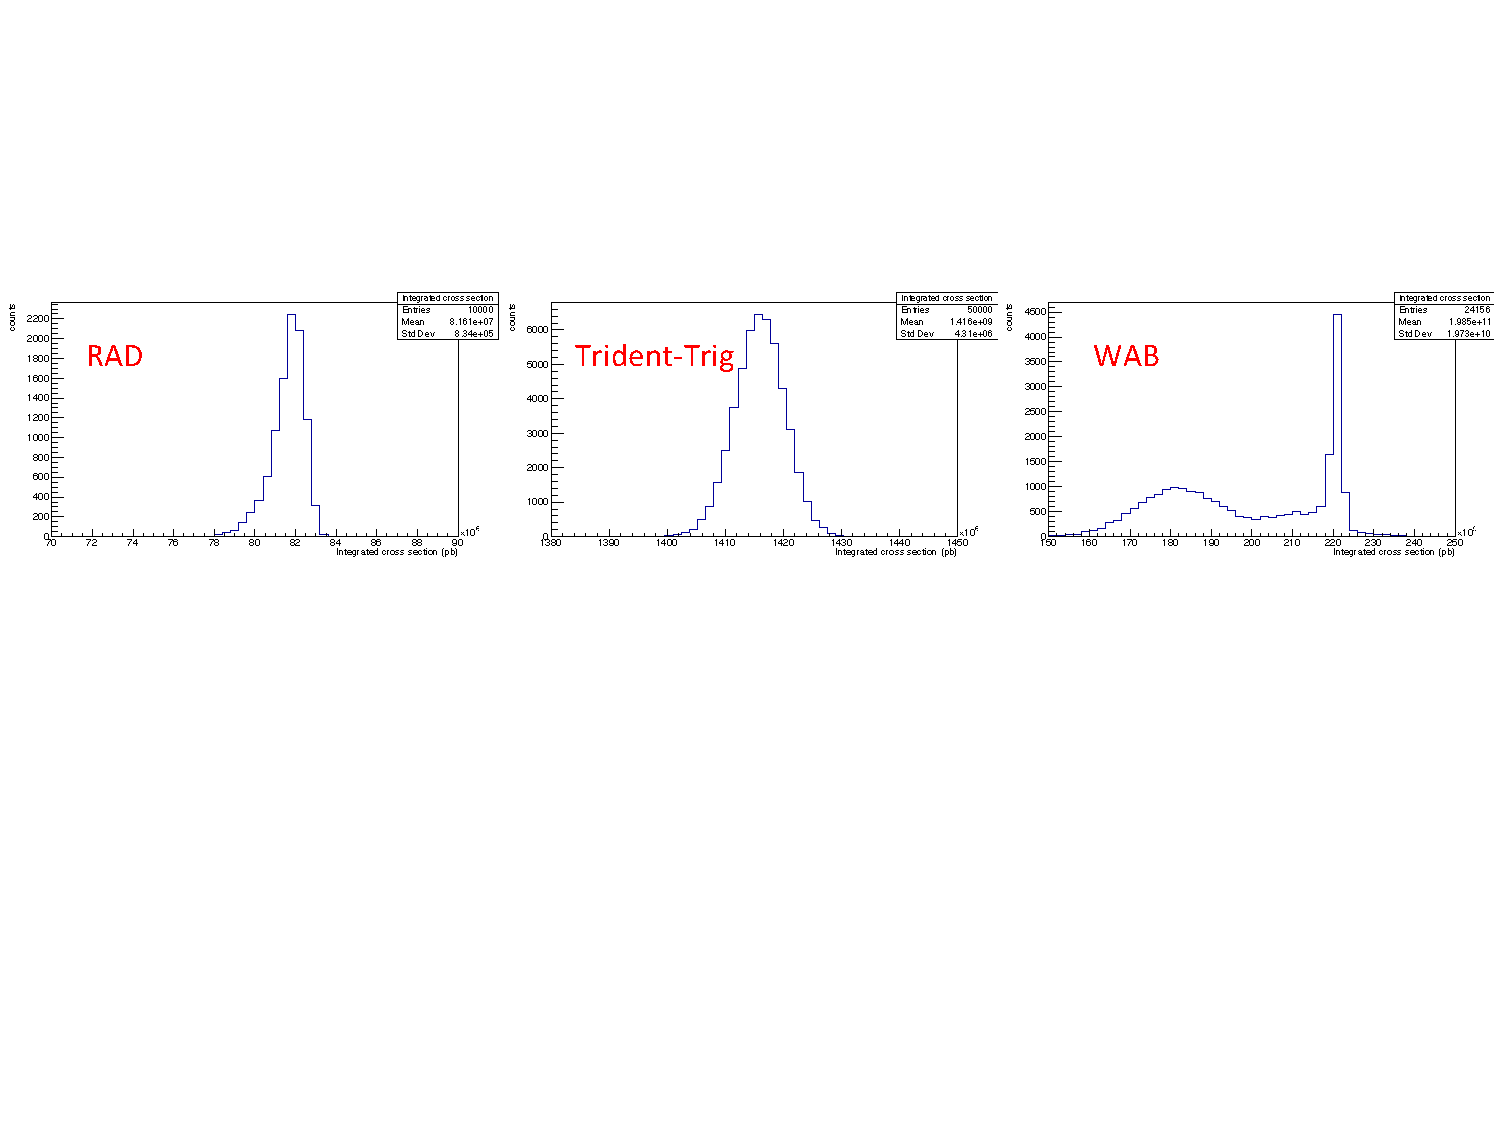
\includegraphics[width=1.\textwidth]{figs/recon/integrated-cross-section-from-MadGraph.pdf}
%    \caption{Integrated cross section for the RAD (left), Trident-Trig(middle) and WAB(right) samples, separately.}
%    \label{fig:integrated_cross_section_from_madgraph}
%\end{figure}

\begin{table}[!hb] 
\centering
\begin{tabular}{ccccc}
   \toprule    
    Sample & $\mu$ of ICS & $\sigma$ of ICS & \# of good files &  \# of generated events per file \\
    \midrule
     RAD & 66.36 $\mu$b & 0.6678 $\mu$b & 9940 & 10k \\
     Trident-Trig & 1.416 mb & 0.004310 mb & 9853 & 50k \\
     WAB & 0.1985 b & 0.01973 b & 9956 & 100k \\
     \bottomrule
\end{tabular}
\caption{Normalization parameters for the RAD, Tritrig, and WAB samples. The mean $\mu$ and the $\sigma$ are obtained from the distribution of integrated cross-sections (ICS) from the individual generated samples.}
\label{table:normalization}
\end{table}

Normalization for MC is computed by using the mean $\mu$ of the integrated cross section (ICS) for each sample produced %as shown in Fig. \ref{fig:integrated_cross_section_from_madgraph} 
and the total number of events generated (Luminosity = Events Generated / Mean ($\mu$) ICS). The results are shown in Table \ref{table:normalization} and are used to separate the rate of different $\epem$ production processes and as a comparison to the overall $\epem$ rate in data. The ICS is computed after the cuts from Tab. \ref{table:MCrequirements}.


\subsection{HPS $\epem$ Rates}\label{sec:rates}
A dedicated study of the HPS $\epem$ composition from MC and overall rate compared with $\epem$ data rates is documented in the 2016 sample composition note \cite{tridentnote2016}. The study looked at both $\gamma e^-$ (dominated by WABs) and $\epem$ (both tridents and cWABs) final states. The MCs used for this are summarized in \ref{sec:mc} and the data used is $\sim$10\% of run 7963. The selection used for the composition study were chosen to be the same as those used in the preselection defined in Tab. \ref{tab:preselection}.

Figure \ref{fig:epem_noESumCut_AllScale} shows the distributions of some kinematic variables for the $\epem$ events from the composition study.  In addition to the preselection, the events shown in these distributions have a minimum $\epem$ momentum sum cut (referred to as the radiative cut in Sec. \ref{sec:apvertexcuts}) but do not require that the tracks have both L1 and L2 hits.  

From these studies, it appears that the MC overestimates the overall $\epem$ rate in data by $\sim20$\%, thus scaling the overall MC cross-section by 80\% shows excellent agreement. 

\begin{figure}[tbhp]
        \centering
      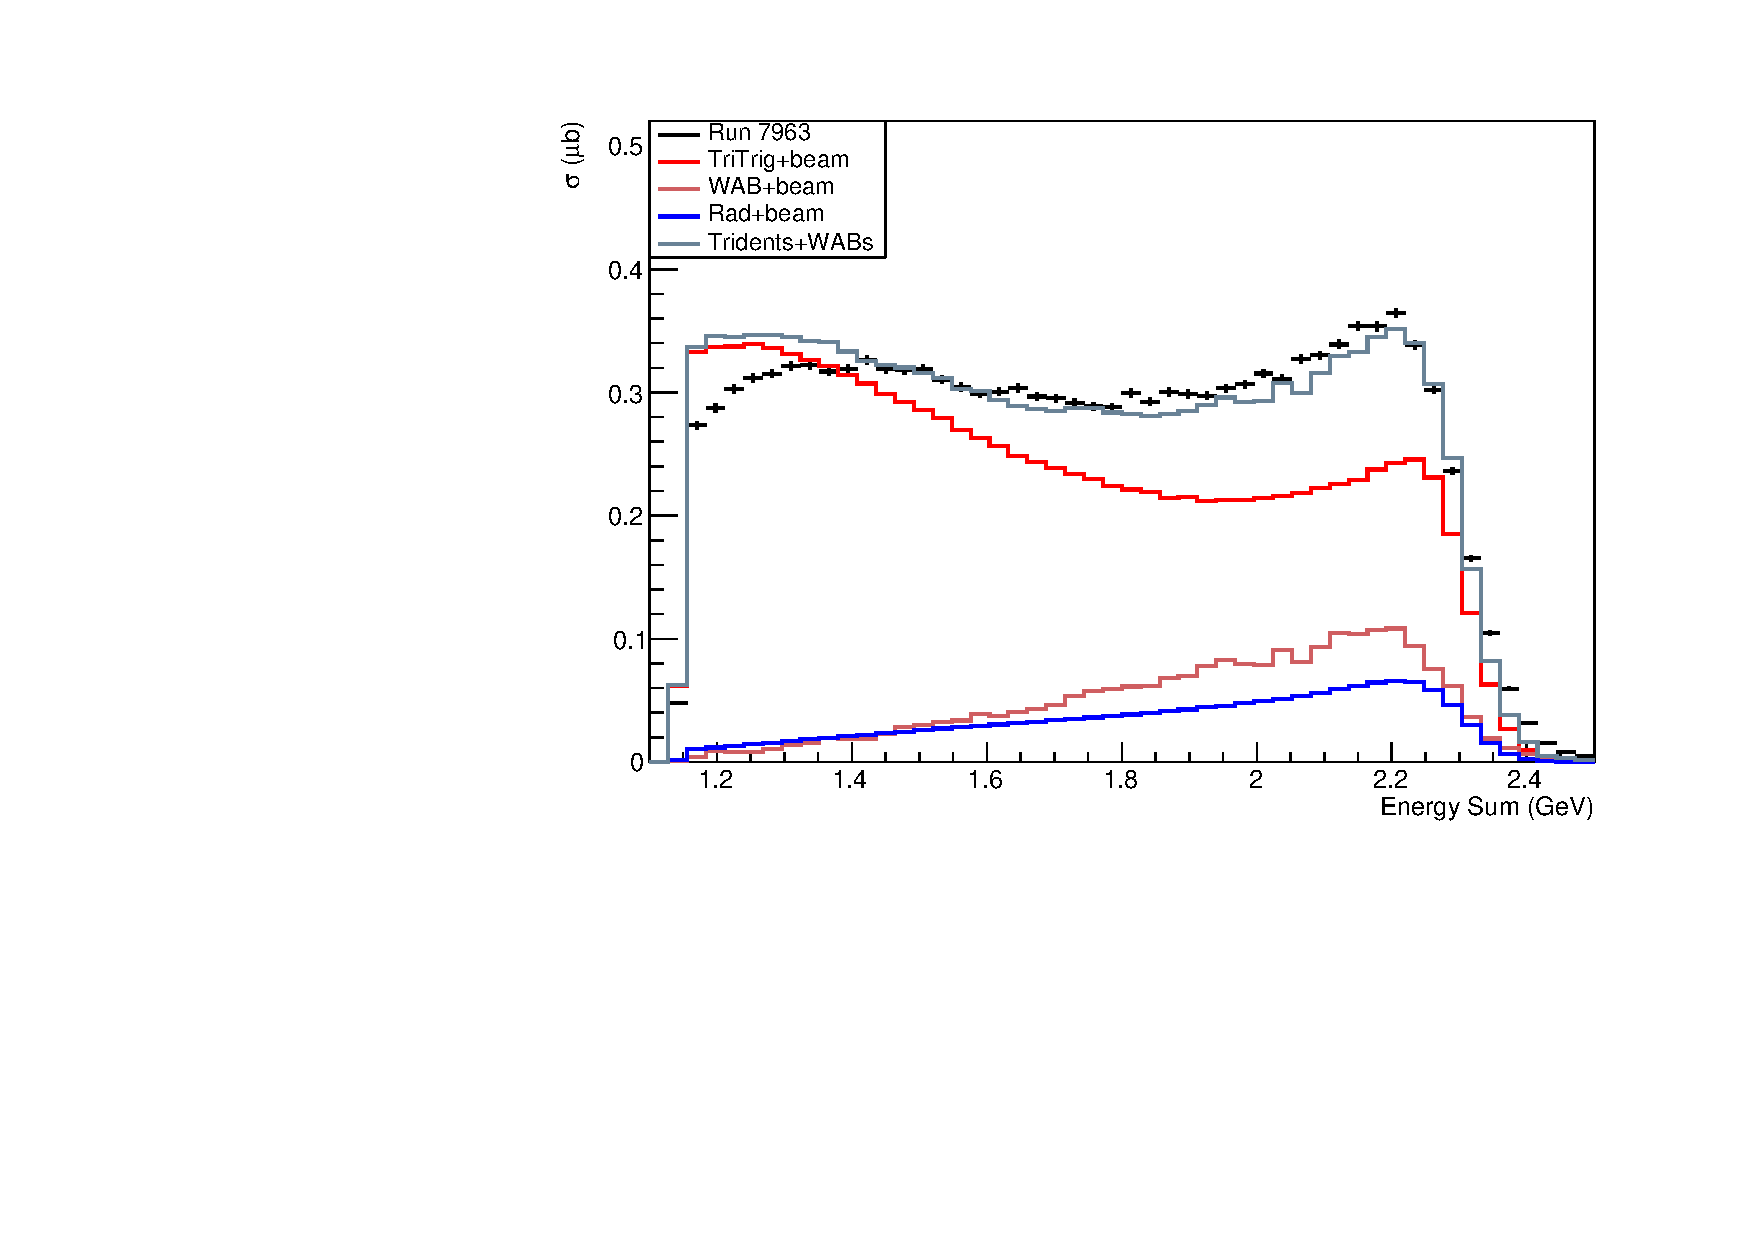
\includegraphics[scale=0.35]{figs/recon/xs-norm-data-EpEmTB-eSum-intruns-NoESumCut_pre-vertex-intplots.pdf}
      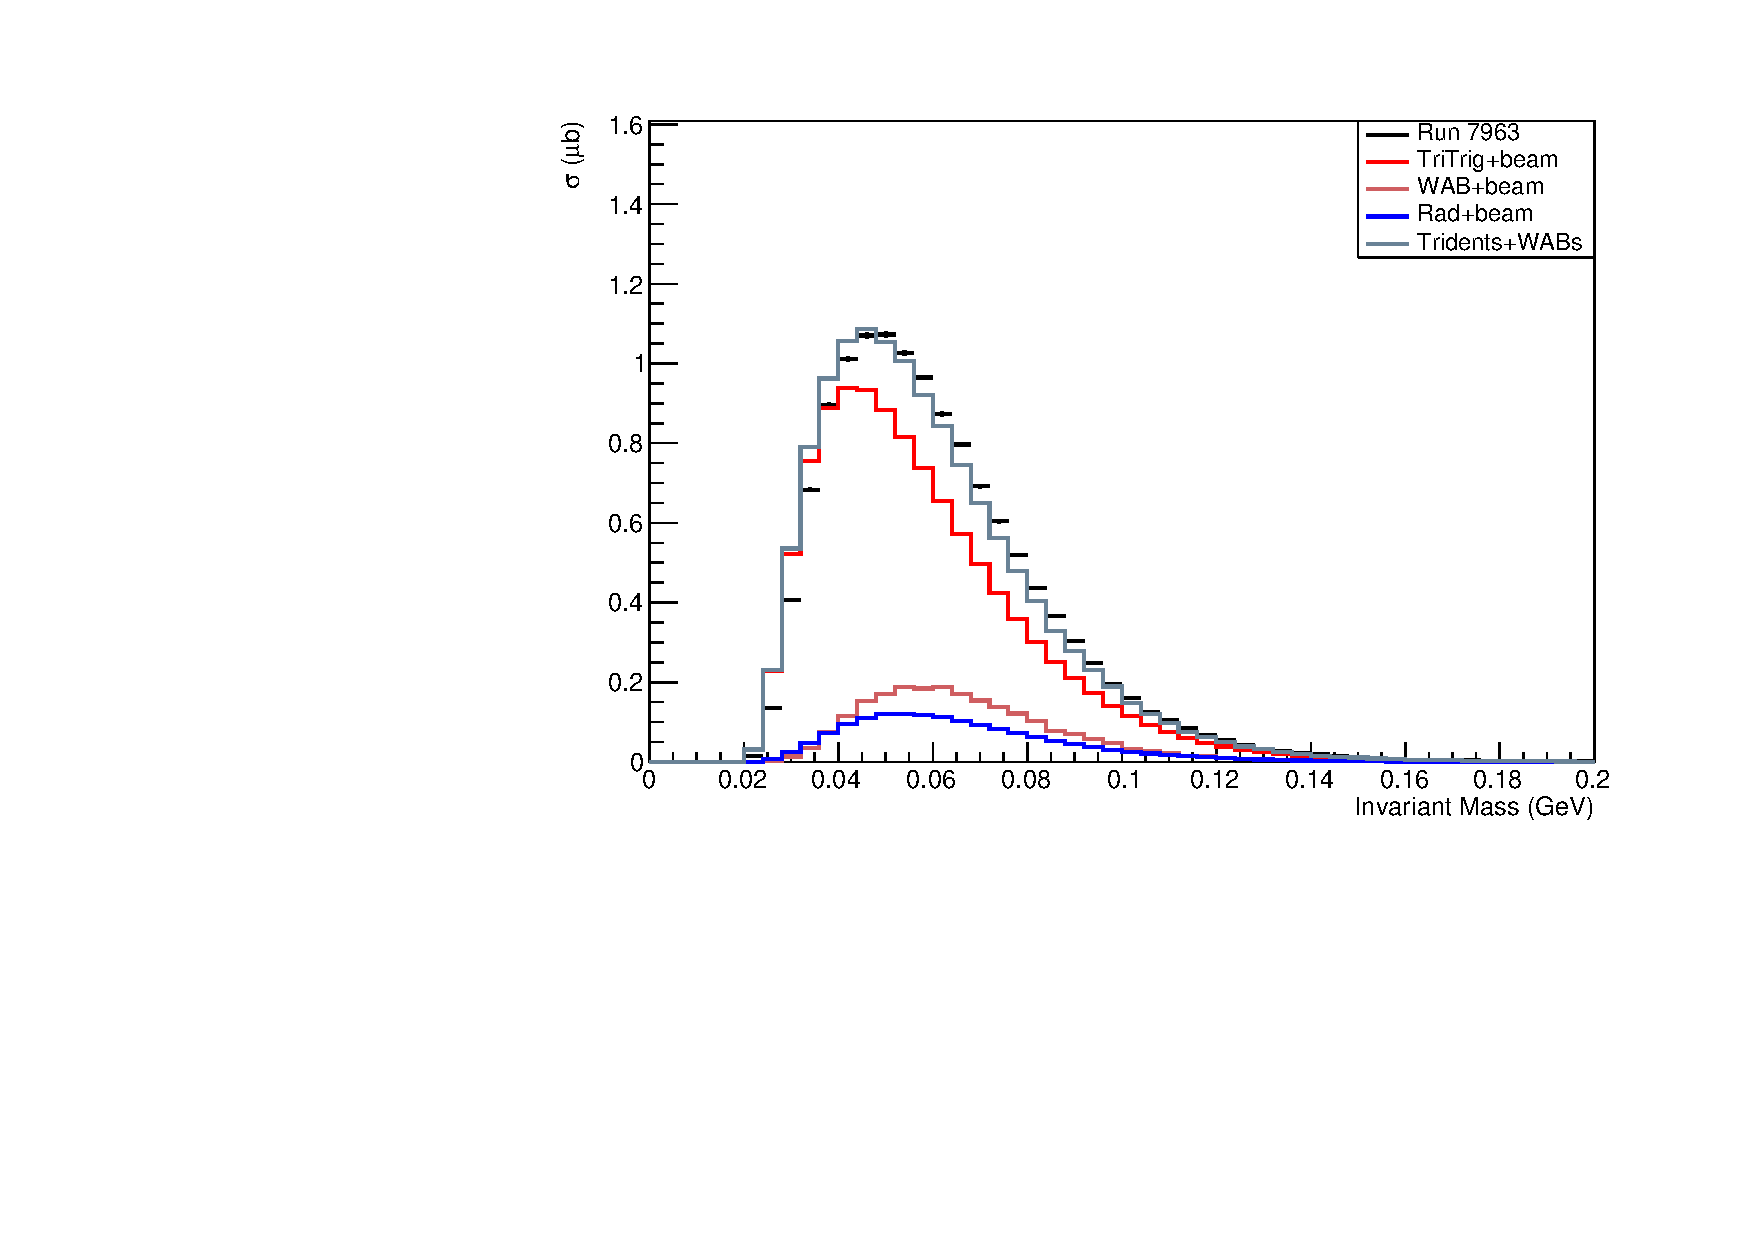
\includegraphics[scale=0.35]{figs/recon/xs-norm-data-EpEmTB-pairMass-intruns-NoESumCut_pre-vertex-intplots.pdf}
      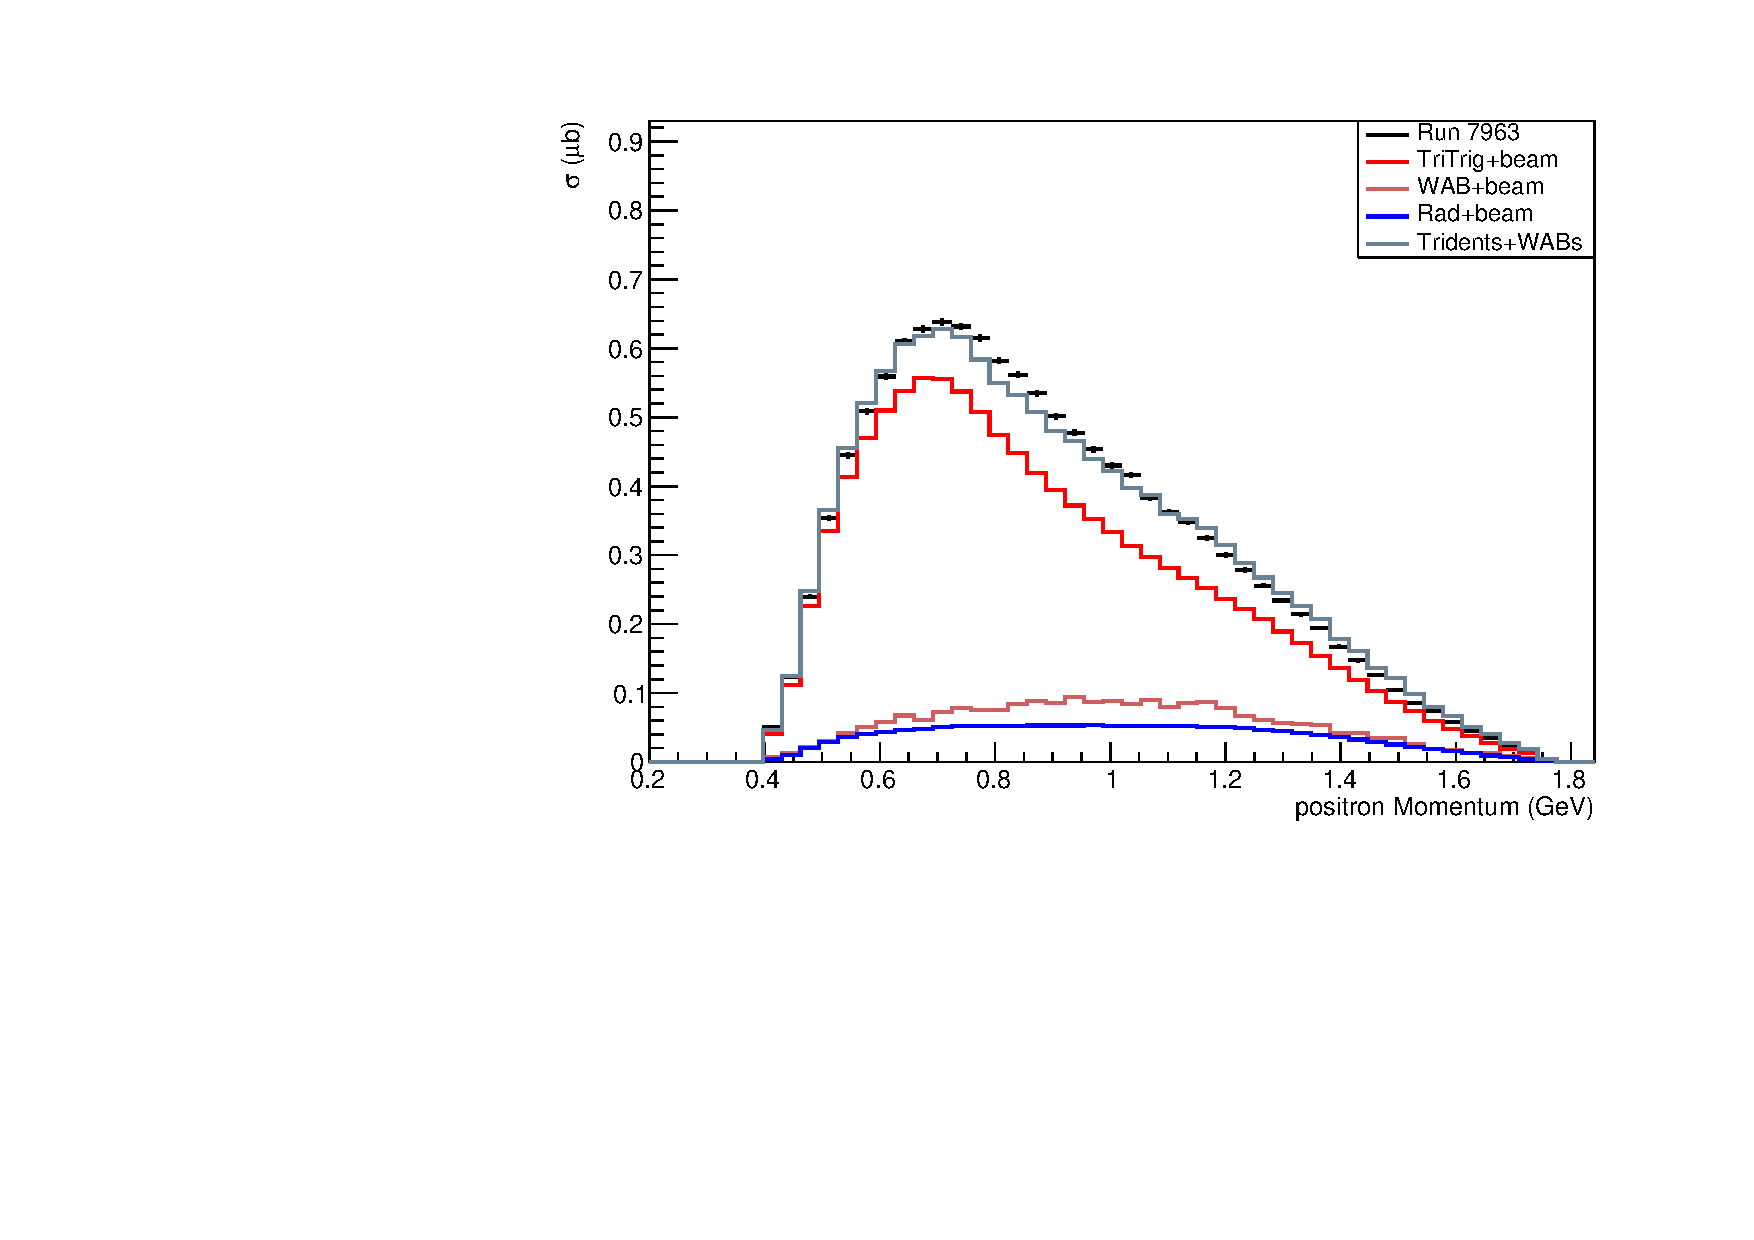
\includegraphics[scale=0.35]{figs/recon/xs-norm-data-EpEmTB-p1Mom-intruns-NoESumCut_pre-vertex-intplots.pdf}
      \includegraphics[scale=0.35]{figs/recon/xs-norm-data-EpEmTB-p1slope-intruns-NoESumCut_pre-vertex-intplots.pdf}
      \includegraphics[scale=0.35]{figs/recon/xs-norm-data-EpEmTB-p2Mom-intruns-NoESumCut_pre-vertex-intplots.pdf}
      \includegraphics[scale=0.35]{figs/recon/xs-norm-data-EpEmTB-p2slope-intruns-NoESumCut_pre-vertex-intplots.pdf}
    \caption{Distributions of $\epem$ events with scaling all MC cross-sections by 0.8. Upper Left: $\epem$ momentum sum. Upper Right: $\epem$ invariant mass. Middle Left: Positron momentum. Middle Right: Positron track slope. Bottom Left: Electron momentum. Bottom Right: Electron track slope.
    %Each plot shows the raw distribution from data and the various MC samples as well as the ratio of data and the sum of WAB-beam and tritrig-beam.  
    }
   \label{fig:epem_noESumCut_AllScale}
\end{figure}  
Generally, the agreement between data and MC for these distributions is reasonable with the exception of a $\sim$20\% overall scale difference which may have several sources.  While the MC is generated with a single set of conditions, there is some run-to-run variation in the $\epem$ rates of order 5\%. In addition, this MC does not account for tracking efficiencies which are of the order of $\sim 10\%$ as well as the hit efficiency effects (particularly in layer 1) described in Sec \ref{sec:hiteff}. There are also a few features in these plots (e.g. skew in track momentum, some differences in track slope) that may be attributed to the same causes as the overall rate discrepancy.

It is an assumption that the overall discrepancy between $\epem$ rates in data and MC are the same as the individual contributions. Thus, the fraction of $\epem$ pairs that are due to radiative tridents are the same in data and MC. In other words, these discrepancies cancel when taking the ratio of rates of different processes.

\clearpage

%\section{Composition of the $\epem$ Sample} \label{sec:comp}

\subsection{Radiative Fraction} \label{sec:radfrac}

\begin{figure}[t]
    \centering
    \includegraphics[width=.45\textwidth]{figs/recon/radfracall.pdf}
    \includegraphics[width=.45\textwidth]{figs/recon/radfrac.pdf}
    \caption{Left: The differential cross sections ($d\sigma/dm$) of wab, trident, and radiative trident components from MC as well as the measured cross section from 10\% of the data. In principle, one would expect the tridents + wabs (turquoise) to agree with data (blue). The discrepancy is explained in Sec. \ref{sec:rates}. Right: The radiative fractions as a function of mass. It is fit to a 5th order polynomial and is used to determine the expected radiative trident rate from the number of e+e- pairs in a mass bin.}
    \label{fig:radfrac}
\end{figure}

A key component to translating the number of signal events to the coupling $\epsilon$ is the fraction of reconstructed events in our sample, after all selection requirements, that come from radiative tridents.  This fraction, the so-called radiative fraction, is defined as a function of mass:

\begin{equation}
f_{rad}(m)=\frac{d\sigma_{rad}/dm(m)}{d\sigma_{tri}/dm(m)+d\sigma_{cWAB}/dm(m)}
\label{eqn:radfrac}
\end{equation}

While the total number of $\epem$ pairs can be taken from data the radiative fraction must be computed using MC. Therefore it is important that the composition of our data sample, namely, the relative contributions of trident events to converted WAB (cWAB) events is understood. 

Each term in Eq. \ref{eqn:radfrac} is computed from MC by taking each individual process after running through the full trigger and detector simulation (which incorporates acceptance and efficiency effects) and weighting it by the cross-section from the respective MC generator. This is done as a function of mass, specifically in narrow mass bins. As stated previously, it is assumed that the overall $\epem$ rate discrepancy between data and MC have negligible effects on the radiative fraction.

%The method of determining the radiative fraction is the same as used in the resonance search. The actual $\epem$ daughter pairs from the $\gamma^*$ for the radiative events (i.e. the numerator in the radiative fraction) are truth-matched to avoid including events that are falsely reconstructed with the recoil electron. %The radiative events that are correctly truth-matched are then planed within a bin of truth mass and used in the numberator of the radiative fraction. 

For the numerator (i.e. the radiative component), the $\epem$ pairs from radiative processes are truth-matched and only events in which the the true $\epem$ daughter pairs reconstruct from the decay of the the $\gamma^*$ are used. This is done to eliminate $\epem$ pairs in which the positron falsely reconstructs with the recoil electron (which gives an incorrect reconstructed mass) and to utilize the truth mass. The truth mass is computed from the invariant mass from these truth-matched $\epem$ pairs using the truth momentum components of the particles. Using the truth mass reduces the systematic uncertainty associated with signal leaking in or out of the narrow mass bins. 

%Thus, for the radiative fraction, the reconstructed masses are used in the denominator which is the background portion expected from data while the numerator uses the truth mass which correctly computes. This reduced the systematic uncertainty associated with signal leaking in or out of the narrow mass bins. 

For the denominator (i.e. the sum of the total trident and converted WAB components), physics does not enable the differentiation between trident events that are reconstructed with the true daughter electron as opposed to the recoil electron (even if using truth information from MC due to the cross terms between the Bethe-Heitler and radiative diagrams). As a result, these events cannot be truth-matched and the reconstructed mass must be used in a mass bin in the denominator. The total denominator is representative of the total composition in data which also must rely on reconstructed masses.

%The total number of tridents and wabs (i.e. the sum of the expected $\epem$ backgrounds) are used in the denominator of the radiative fraction. Since physics does not enable us to differentiate between trident events that are reconstructed with the true daughter electron as opposed to the recoil electron (even using truth information from MC due to the cross terms between the Bethe-Heitler and radiative diagrams), these events cannot be truth-matched and the reconstructed mass is used in a mass bin in the denominator.

\begin{figure}[t]
    \centering
    \includegraphics[width=.45\textwidth]{figs/recon/invmass.pdf}
    \includegraphics[width=.45\textwidth]{figs/recon/radfrac_unblind.pdf}
    \caption{The invariant mass for Left: 10\% of the data and Right: 100\% of the data with the radiative cut selection. It is fitted to an exponential to a 5th order polynomial. This is the number of e+e- pairs in a 1 MeV bin used to normalize the expected radiative trident rate, and hence the expected A' rate.}
    \label{fig:inv_mass}
\end{figure}

%The two notable differences between the displaced vertex search and the resonance search with respect to the radiative fraction are the event selection and the use of unconstrained vertices as opposed to target constrained in the resonance search. The selection that is used for the radiative fraction for the displaced vertex search are the preselection cuts from Sec. \ref{sec:selection} as well as the layer 2 requirement, and the radiative cut (V0 momentum) is shown in Table \ref{tab:radfrac}. When deriving the expected $A'$ rate, the added complication of the displaced vertex search is the fact that the analysis is divided into several mutually exclusive categories based on the first layer with a hit on track, and each of these categories has a different selection. The motivation for these specific cuts is to use only the cuts that are shared between these categories. The isolation cut, impact parameter cut, and V0 projection back to the target are applied in a later step.

%The selection that is used for the radiative fraction for the displaced vertex search are the preselection cuts from Sec. \ref{sec:preselection} as well as the layer 2 requirement, and the $\epem$ momentum sum cut (radiative cut) is shown in Table \ref{tab:radfrac}. %When deriving the expected $A'$ rate, the added complication of the displaced vertex search is the fact that the analysis is divided into several mutually exclusive categories based on the first layer with a hit on track, and each of these categories has a different selection. The motivation for these specific cuts is to use only the cuts that are shared between these categories. The isolation cut, impact parameter cut, and V0 projection back to the target are applied in a later step.

\begin{table}[!hb] 
    \centering
    \begin{tabular}{lr}
        \toprule
        \textbf{Cut Description} & \textbf{Requirement} \\
        \midrule
        Preselection & - \\
        Layer 2 Requirement & $e^+$ and $e^-$ have L2 hit \\
        %Tight Vertex Quality & $\chi^2_{unc} < 4$ \\
        Radiative Cut & $V_{0p} > 1.85$ GeV \\
        \bottomrule
    \end{tabular}
    \caption{A list of cuts that are used before determining the radiative fraction and the number of e+e- events within a mass bin. The cuts are composed of the preselection cuts from Sec. \ref{sec:preselection} with the addition of a few extra cuts including the radiative cut (the cut on $\epem$ momentum sum).}
    \label{tab:radfrac}
\end{table}

The selection that is used for the radiative fraction for the displaced vertex search are the preselection cuts from Sec. \ref{sec:preselection} as well as the layer 2 requirement and the $\epem$ momentum sum cut (radiative cut) and is shown in Table \ref{tab:radfrac}. From these selections, the radiative fraction is computed as the number of truth-matched radiative tridents in a narrow bin of truth mass divided by the sum of trident and WAB processes in the same narrow bin of reconstructed mass, and normalized by their cross-sections, as a function of mass as in Eq. \ref{eqn:radfrac}. Both the radiative fraction and differential cross sections of various background components and data are shown in Fig. \ref{fig:radfrac}. The radiative fraction is parametrized using a 5th order polynomial.

\begin{equation}
f_{rad}(m[\mthrm{GeV}])= 0.1168-1.375m + 10.19m^2 +9.422m^3 -367.5 m^4 -1023 m^5
\label{eqn:radfrac_param}
\end{equation}

%Using the radiative fraction and the number of e+e- pairs in a given mass bin will give the expected number of radiative tridents in that mass bin, the $N_{bin}$ in Eq. \ref{eqn:signal_yield} ($N_{rad}(m)=f_{rad}(m) N_{bin}(m)$). The invariant mass plot using the radiative fraction selection from Table \ref{tab:radfrac} using 1 MeV bins which gives the number of e+e- events in that bin is shown in Fig. \ref{fig:inv_mass}. This is parametrized as using an exponential to a 5th order polynomial.

Using the radiative fraction and the number of e+e- pairs in a given narrow mass bin $N_{bin}$ will provide a way to compute the expected number of radiative tridents in that mass bin ($N_{rad}(m)=f_{rad}(m) N_{bin}(m)$). The invariant mass plot using the radiative fraction selection from Table \ref{tab:radfrac} using 1 MeV bins ($\delta m_{\aprime}$), which gives the number of e+e- events in that bin, is shown in Fig. \ref{fig:inv_mass}. This is parametrized as using an exponential to a 5th order polynomial. For the 10\% blinded sample this gives

\begin{equation}
N_{bin}(m[\mathrm{GeV}])=e^{ 4.903+208.3m -1880m^2 -1868m^3 + 6.870e4m^4 -1.980e5 m^5}
\label{eqn:num_param}
\end{equation}

and for the full 100\% of the data this gives

\begin{equation}
N_{bin}(m[\mathrm{GeV}])=e^{ 6.309+328.4m -5099m^2 +3.675e4m^3 -1.492e5m^4 +2.724e5 m^5}
\label{eqn:num_param2}
\end{equation}

Using these equations and the radiative fraction, the expected number of radiative tridents in a given mass bin can be computed. From there, rearranging Eq. \ref{eqn:radiatives} gives the expected $\aprime$ production rate at the target within the detector acceptance as a function of mass and $\epsilon$. 

\begin{equation}
S(m_{A'},\epsilon)=f_{rad} N_{bin} \frac{3\pi \epsilon^2}{2N_{eff} \alpha} \frac{m_{A'}}{\delta m_{A'}} 
    \label{eqn:signal_prod}
\end{equation}

This result normalized to both 10\% of the dataset and the full dataset is shown in Fig. \ref{fig:ap_yield}. The last step is to displace the $\aprime$s over a range in $z$ based on their expected decay distributions and then perform the proper accounting based on whether or not the $\epem$ pair is within acceptance of layer 1 while correctly incorporating hit efficiency effects and tighter selection cuts. This is discussed in detail in Sec. \ref{sec:hitkill}.

\begin{figure}[t]
    \centering
    \includegraphics[width=.85\textwidth]{figs/Results/ap_produced.pdf}
    \includegraphics[width=.85\textwidth]{figs/recon/ap_produced_unblind.pdf}
    \caption{Top: The number of A's produced for each mass and $\epsilon^2$ in prompt acceptance including all efficiencies for 10\% of the data. In other words, the term in front of the integral in Eq. \ref{eqn:signal_yield}. Bottom: The number of A's produced for each mass and $\epsilon^2$ in prompt acceptance including all efficiencies for 100\% of the data.
    }
    \label{fig:ap_yield}
\end{figure}

\clearpage